
%----------------------------------------------------------------------------------------
%	PACKAGES AND OTHER DOCUMENT CONFIGURATIONS
%----------------------------------------------------------------------------------------

\documentclass[11pt,fleqn]{book} % Default font size and left-justified equations

%----------------------------------------------------------------------------------------

%%%%%%%%%%%%%%%%%%%%%%%%%%%%%%%%%%%%%%%%%
% The Legrand Orange Book
% Structural Definitions File
% Version 2.0 (9/2/15)
%
% Original author:
% Mathias Legrand (legrand.mathias@gmail.com) with modifications by:
% Vel (vel@latextemplates.com)
% 
% This file has been downloaded from:
% http://www.LaTeXTemplates.com
%
% License:
% CC BY-NC-SA 3.0 (http://creativecommons.org/licenses/by-nc-sa/3.0/)
%
%%%%%%%%%%%%%%%%%%%%%%%%%%%%%%%%%%%%%%%%%
\usepackage{pdfpages}
\usepackage{wrapfig}
\usepackage{booktabs}

%----------------------------------------------------------------------------------------
%	VARIOUS REQUIRED PACKAGES AND CONFIGURATIONS
%----------------------------------------------------------------------------------------
\usepackage{float}
\usepackage{caption}
\usepackage[top=3cm,bottom=3cm,left=3cm,right=3cm,headsep=10pt,a4paper]{geometry} % Page margins
\usepackage{minted}
\usepackage{graphicx} % Required for including pictures
\graphicspath{{Pictures/}} % Specifies the directory where pictures are stored
\usepackage{listings}
\usepackage{lipsum} % Inserts dummy text

\usepackage{tikz} % Required for drawing custom shapes

\usepackage[french]{babel} % English language/hyphenation

\usepackage{enumitem} % Customize lists
\setlist{nolistsep} % Reduce spacing between bullet points and numbered lists

\usepackage{booktabs} % Required for nicer horizontal rules in tables

\usepackage{xcolor} % Required for specifying colors by name
\definecolor{ocre}{RGB}{113, 153, 255} % Define the orange color used for highlighting throughout the book

%----------------------------------------------------------------------------------------
%	FONTS
%----------------------------------------------------------------------------------------

%\usepackage{avant} % Use the Avantgarde font for headings
\usepackage{times} % Use the Times font for headings
\usepackage{mathptmx} % Use the Adobe Times Roman as the default text font together with math symbols from the Sym­bol, Chancery and Com­puter Modern fonts

\usepackage{microtype} % Slightly tweak font spacing for aesthetics
\usepackage[utf8]{inputenc} % Required for including letters with accents
\usepackage[T1]{fontenc} % Use 8-bit encoding that has 256 glyphs

%----------------------------------------------------------------------------------------
%	BIBLIOGRAPHY AND INDEX
%----------------------------------------------------------------------------------------

\usepackage{csquotes}
\usepackage[backend=biber]{biblatex}
\addbibresource{bibliography.bib} % BibTeX bibliography file
\defbibheading{bibempty}{}

\usepackage{calc} % For simpler calculation - used for spacing the index letter headings correctly
\usepackage{makeidx} % Required to make an index
\makeindex % Tells LaTeX to create the files required for indexing

%----------------------------------------------------------------------------------------
%	MAIN TABLE OF CONTENTS
%----------------------------------------------------------------------------------------

\usepackage{titletoc} % Required for manipulating the table of contents
\usepackage{titlepic}
\contentsmargin{0cm} % Removes the default margin
\addtocontents{toc}{\vspace{-2cm}}

% Part text styling
\titlecontents{part}[0cm]
{\addvspace{20pt}\centering\large\bfseries}
{}
{}
{}

% Chapter text styling
\titlecontents{chapter}[1.25cm] % Indentation
{\addvspace{12pt}\large\sffamily\bfseries} % Spacing and font options for chapters
{\color{ocre!60}\contentslabel[\Large\thecontentslabel]{1.25cm}\color{ocre}} % Chapter number
{\color{ocre}}  
{\color{ocre!60}\normalsize\;\titlerule*[.5pc]{.}\;\thecontentspage} % Page number

% Section text styling
\titlecontents{section}[1.25cm] % Indentation
{\addvspace{3pt}\sffamily\bfseries} % Spacing and font options for sections
{\contentslabel[\thecontentslabel]{1.25cm}} % Section number
{}
{\hfill\color{black}\thecontentspage} % Page number
[]

% Subsection text styling
\titlecontents{subsection}[1.25cm] % Indentation
{\addvspace{1pt}\sffamily\small} % Spacing and font options for subsections
{\contentslabel[\thecontentslabel]{1.25cm}} % Subsection number
{}
{\ \titlerule*[.5pc]{.}\;\thecontentspage} % Page number
[]

% List of figures
\titlecontents{figure}[0em]
{\addvspace{-5pt}\sffamily}
{\thecontentslabel\hspace*{1em}}
{}
{\ \titlerule*[.5pc]{.}\;\thecontentspage}
[]

% List of tables
\titlecontents{table}[0em]
{\addvspace{-5pt}\sffamily}
{\thecontentslabel\hspace*{1em}}
{}
{\ \titlerule*[.5pc]{.}\;\thecontentspage}
[]

%----------------------------------------------------------------------------------------
%	MINI TABLE OF CONTENTS IN PART HEADS
%----------------------------------------------------------------------------------------

% Chapter text styling
\titlecontents{lchapter}[0em] % Indenting
{\addvspace{15pt}\large\sffamily\bfseries} % Spacing and font options for chapters
{\color{ocre}\contentslabel[\Large\thecontentslabel]{1.25cm}\color{ocre}} % Chapter number
{}  
{\color{ocre}\normalsize\sffamily\bfseries\;\titlerule*[.5pc]{.}\;\thecontentspage} % Page number

% Section text styling
\titlecontents{lsection}[0em] % Indenting
{\sffamily\small} % Spacing and font options for sections
{\contentslabel[\thecontentslabel]{1.25cm}} % Section number
{}
{}

% Subsection text styling
\titlecontents{lsubsection}[.5em] % Indentation
{\normalfont\footnotesize\sffamily} % Font settings
{}
{}
{}

%----------------------------------------------------------------------------------------
%	PAGE HEADERS
%----------------------------------------------------------------------------------------

\usepackage{fancyhdr} % Required for header and footer configuration

\pagestyle{fancy}
\renewcommand{\chaptermark}[1]{\markboth{\sffamily\normalsize\bfseries\chaptername\ \thechapter.\ #1}{}} % Chapter text font settings
\renewcommand{\sectionmark}[1]{\markright{\sffamily\normalsize\thesection\hspace{5pt}#1}{}} % Section text font settings
\fancyhf{} \fancyhead[LE,RO]{\sffamily\normalsize\thepage} % Font setting for the page number in the header
\fancyhead[LO]{\rightmark} % Print the nearest section name on the left side of odd pages
\fancyhead[RE]{\leftmark} % Print the current chapter name on the right side of even pages
\renewcommand{\headrulewidth}{0.5pt} % Width of the rule under the header
\addtolength{\headheight}{2.5pt} % Increase the spacing around the header slightly
\renewcommand{\footrulewidth}{0pt} % Removes the rule in the footer
\fancypagestyle{plain}{\fancyhead{}\renewcommand{\headrulewidth}{0pt}} % Style for when a plain pagestyle is specified

% Removes the header from odd empty pages at the end of chapters
\makeatletter
\renewcommand{\cleardoublepage}{
\clearpage\ifodd\c@page\else
\hbox{}
\vspace*{\fill}
\thispagestyle{empty}
\newpage
\fi}

%----------------------------------------------------------------------------------------
%	THEOREM STYLES
%----------------------------------------------------------------------------------------

\usepackage{amsmath,amsfonts,amssymb,amsthm} % For math equations, theorems, symbols, etc

\newcommand{\intoo}[2]{\mathopen{]}#1\,;#2\mathclose{[}}
\newcommand{\ud}{\mathop{\mathrm{{}d}}\mathopen{}}
\newcommand{\intff}[2]{\mathopen{[}#1\,;#2\mathclose{]}}
\newtheorem{notation}{Notation}[chapter]

% Boxed/framed environments
\newtheoremstyle{ocrenumbox}% % Theorem style name
{0pt}% Space above
{0pt}% Space below
{\normalfont}% % Body font
{}% Indent amount
{\small\bf\sffamily\color{ocre}}% % Theorem head font
{\;}% Punctuation after theorem head
{0.25em}% Space after theorem head
{\small\sffamily\color{ocre}\thmname{#1}\nobreakspace\thmnumber{\@ifnotempty{#1}{}\@upn{#2}}% Theorem text (e.g. Theorem 2.1)
\thmnote{\nobreakspace\the\thm@notefont\sffamily\bfseries\color{black}---\nobreakspace#3.}} % Optional theorem note
\renewcommand{\qedsymbol}{$\blacksquare$}% Optional qed square

\newtheoremstyle{blacknumex}% Theorem style name
{5pt}% Space above
{5pt}% Space below
{\normalfont}% Body font
{} % Indent amount
{\small\bf\sffamily}% Theorem head font
{\;}% Punctuation after theorem head
{0.25em}% Space after theorem head
{\small\sffamily{\tiny\ensuremath{\blacksquare}}\nobreakspace\thmname{#1}\nobreakspace\thmnumber{\@ifnotempty{#1}{}\@upn{#2}}% Theorem text (e.g. Theorem 2.1)
\thmnote{\nobreakspace\the\thm@notefont\sffamily\bfseries---\nobreakspace#3.}}% Optional theorem note

\newtheoremstyle{blacknumbox} % Theorem style name
{0pt}% Space above
{0pt}% Space below
{\normalfont}% Body font
{}% Indent amount
{\small\bf\sffamily}% Theorem head font
{\;}% Punctuation after theorem head
{0.25em}% Space after theorem head
{\small\sffamily\thmname{#1}\nobreakspace\thmnumber{\@ifnotempty{#1}{}\@upn{#2}}% Theorem text (e.g. Theorem 2.1)
\thmnote{\nobreakspace\the\thm@notefont\sffamily\bfseries---\nobreakspace#3.}}% Optional theorem note

% Non-boxed/non-framed environments
\newtheoremstyle{ocrenum}% % Theorem style name
{5pt}% Space above
{5pt}% Space below
{\normalfont}% % Body font
{}% Indent amount
{\small\bf\sffamily\color{ocre}}% % Theorem head font
{\;}% Punctuation after theorem head
{0.25em}% Space after theorem head
{\small\sffamily\color{ocre}\thmname{#1}\nobreakspace\thmnumber{\@ifnotempty{#1}{}\@upn{#2}}% Theorem text (e.g. Theorem 2.1)
\thmnote{\nobreakspace\the\thm@notefont\sffamily\bfseries\color{black}---\nobreakspace#3.}} % Optional theorem note
\renewcommand{\qedsymbol}{$\blacksquare$}% Optional qed square
\makeatother

% Defines the theorem text style for each type of theorem to one of the three styles above
\newcounter{dummy} 
\numberwithin{dummy}{section}
\theoremstyle{ocrenumbox}
\newtheorem{theoremeT}[dummy]{Theorem}
\newtheorem{problem}{Problem}[chapter]
\newtheorem{exerciseT}{Exercise}[chapter]
\theoremstyle{blacknumex}
\newtheorem{exampleT}{Example}[chapter]
\theoremstyle{blacknumbox}
\newtheorem{vocabulary}{Vocabulary}[chapter]
\newtheorem{definitionT}{Definition}[section]
\newtheorem{corollaryT}[dummy]{Corollary}
\theoremstyle{ocrenum}
\newtheorem{proposition}[dummy]{Proposition}

%----------------------------------------------------------------------------------------
%	DEFINITION OF COLORED BOXES
%----------------------------------------------------------------------------------------

\RequirePackage[framemethod=default]{mdframed} % Required for creating the theorem, definition, exercise and corollary boxes

% Theorem box
\newmdenv[skipabove=7pt,
skipbelow=7pt,
backgroundcolor=black!5,
linecolor=ocre,
innerleftmargin=5pt,
innerrightmargin=5pt,
innertopmargin=5pt,
leftmargin=0cm,
rightmargin=0cm,
innerbottommargin=5pt]{tBox}

% Exercise box	  
\newmdenv[skipabove=7pt,
skipbelow=7pt,
rightline=false,
leftline=true,
topline=false,
bottomline=false,
backgroundcolor=ocre!10,
linecolor=ocre,
innerleftmargin=5pt,
innerrightmargin=5pt,
innertopmargin=5pt,
innerbottommargin=5pt,
leftmargin=0cm,
rightmargin=0cm,
linewidth=4pt]{eBox}	

% Definition box
\newmdenv[skipabove=7pt,
skipbelow=7pt,
rightline=false,
leftline=true,
topline=false,
bottomline=false,
linecolor=ocre,
innerleftmargin=5pt,
innerrightmargin=5pt,
innertopmargin=0pt,
leftmargin=0cm,
rightmargin=0cm,
linewidth=4pt,
innerbottommargin=0pt]{dBox}	

% Corollary box
\newmdenv[skipabove=7pt,
skipbelow=7pt,
rightline=false,
leftline=true,
topline=false,
bottomline=false,
linecolor=gray,
backgroundcolor=black!5,
innerleftmargin=5pt,
innerrightmargin=5pt,
innertopmargin=5pt,
leftmargin=0cm,
rightmargin=0cm,
linewidth=4pt,
innerbottommargin=5pt]{cBox}

% Creates an environment for each type of theorem and assigns it a theorem text style from the "Theorem Styles" section above and a colored box from above
\newenvironment{theorem}{\begin{tBox}\begin{theoremeT}}{\end{theoremeT}\end{tBox}}
\newenvironment{exercise}{\begin{eBox}\begin{exerciseT}}{\hfill{\color{ocre}\tiny\ensuremath{\blacksquare}}\end{exerciseT}\end{eBox}}				  
\newenvironment{definition}{\begin{dBox}\begin{definitionT}}{\end{definitionT}\end{dBox}}	
\newenvironment{example}{\begin{exampleT}}{\hfill{\tiny\ensuremath{\blacksquare}}\end{exampleT}}		
\newenvironment{corollary}{\begin{cBox}\begin{corollaryT}}{\end{corollaryT}\end{cBox}}	

%----------------------------------------------------------------------------------------
%	REMARK ENVIRONMENT
%----------------------------------------------------------------------------------------

\newenvironment{remark}{\par\vspace{10pt}\small % Vertical white space above the remark and smaller font size
\begin{list}{}{
\leftmargin=35pt % Indentation on the left
\rightmargin=25pt}\item\ignorespaces % Indentation on the right
\makebox[-2.5pt]{\begin{tikzpicture}[overlay]
\node[draw=ocre!60,line width=1pt,circle,fill=ocre!25,font=\sffamily\bfseries,inner sep=2pt,outer sep=0pt] at (-15pt,0pt){\textcolor{ocre}{R}};\end{tikzpicture}} % Orange R in a circle
\advance\baselineskip -1pt}{\end{list}\vskip5pt} % Tighter line spacing and white space after remark

%----------------------------------------------------------------------------------------
%	SECTION NUMBERING IN THE MARGIN
%----------------------------------------------------------------------------------------

\makeatletter
\renewcommand{\@seccntformat}[1]{\llap{\textcolor{ocre}{\csname the#1\endcsname}\hspace{1em}}}                    
\renewcommand{\section}{\@startsection{section}{1}{\z@}
{-4ex \@plus -1ex \@minus -.4ex}
{1ex \@plus.2ex }
{\normalfont\large\sffamily\bfseries}}
\renewcommand{\subsection}{\@startsection {subsection}{2}{\z@}
{-3ex \@plus -0.1ex \@minus -.4ex}
{0.5ex \@plus.2ex }
{\normalfont\sffamily\bfseries}}
\renewcommand{\subsubsection}{\@startsection {subsubsection}{3}{\z@}
{-2ex \@plus -0.1ex \@minus -.2ex}
{.2ex \@plus.2ex }
{\normalfont\small\sffamily\bfseries}}                        
\renewcommand\paragraph{\@startsection{paragraph}{4}{\z@}
{-2ex \@plus-.2ex \@minus .2ex}
{.1ex}
{\normalfont\small\sffamily\bfseries}}

%----------------------------------------------------------------------------------------
%	PART HEADINGS
%----------------------------------------------------------------------------------------

% numbered part in the table of contents
\newcommand{\@mypartnumtocformat}[2]{%
\setlength\fboxsep{0pt}%
\noindent\colorbox{ocre!20}{\strut\parbox[c][.7cm]{\ecart}{\color{ocre!70}\Large\sffamily\bfseries\centering#1}}\hskip\esp\colorbox{ocre!40}{\strut\parbox[c][.7cm]{\linewidth-\ecart-\esp}{\Large\sffamily\centering#2}}}%
%%%%%%%%%%%%%%%%%%%%%%%%%%%%%%%%%%
% unnumbered part in the table of contents
\newcommand{\@myparttocformat}[1]{%
\setlength\fboxsep{0pt}%
\noindent\colorbox{ocre!40}{\strut\parbox[c][.7cm]{\linewidth}{\Large\sffamily\centering#1}}}%
%%%%%%%%%%%%%%%%%%%%%%%%%%%%%%%%%%
\newlength\esp
\setlength\esp{4pt}
\newlength\ecart
\setlength\ecart{1.2cm-\esp}
\newcommand{\thepartimage}{}%
\newcommand{\partimage}[1]{\renewcommand{\thepartimage}{#1}}%
\def\@part[#1]#2{%
\ifnum \c@secnumdepth >-2\relax%
\refstepcounter{part}%
\addcontentsline{toc}{part}{\texorpdfstring{\protect\@mypartnumtocformat{\thepart}{#1}}{\partname~\thepart\ ---\ #1}}
\else%
\addcontentsline{toc}{part}{\texorpdfstring{\protect\@myparttocformat{#1}}{#1}}%
\fi%
\startcontents%
\markboth{}{}%
{\thispagestyle{empty}%
\begin{tikzpicture}[remember picture,overlay]%
\node at (current page.north west){\begin{tikzpicture}[remember picture,overlay]%	
\fill[ocre!20](0cm,0cm) rectangle (\paperwidth,-\paperheight);
\node[anchor=north] at (4cm,-3.25cm){\color{ocre!40}\fontsize{220}{100}\sffamily\bfseries\@Roman\c@part}; 
\node[anchor=south east] at (\paperwidth-1cm,-\paperheight+1cm){\parbox[t][][t]{8.5cm}{
\printcontents{l}{0}{\setcounter{tocdepth}{1}}%
}};
\node[anchor=north east] at (\paperwidth-1.5cm,-3.25cm){\parbox[t][][t]{15cm}{\strut\raggedleft\color{white}\fontsize{30}{30}\sffamily\bfseries#2}};
\end{tikzpicture}};
\end{tikzpicture}}%
\@endpart}
\def\@spart#1{%
\startcontents%
\phantomsection
{\thispagestyle{empty}%
\begin{tikzpicture}[remember picture,overlay]%
\node at (current page.north west){\begin{tikzpicture}[remember picture,overlay]%	
\fill[ocre!20](0cm,0cm) rectangle (\paperwidth,-\paperheight);
\node[anchor=north east] at (\paperwidth-1.5cm,-3.25cm){\parbox[t][][t]{15cm}{\strut\raggedleft\color{white}\fontsize{30}{30}\sffamily\bfseries#1}};
\end{tikzpicture}};
\end{tikzpicture}}
\addcontentsline{toc}{part}{\texorpdfstring{%
\setlength\fboxsep{0pt}%
\noindent\protect\colorbox{ocre!40}{\strut\protect\parbox[c][.7cm]{\linewidth}{\Large\sffamily\protect\centering #1\quad\mbox{}}}}{#1}}%
\@endpart}
\def\@endpart{\vfil\newpage
\if@twoside
\if@openright
\null
\thispagestyle{empty}%
\newpage
\fi
\fi
\if@tempswa
\twocolumn
\fi}

%----------------------------------------------------------------------------------------
%	CHAPTER HEADINGS
%----------------------------------------------------------------------------------------

% A switch to conditionally include a picture, implemented by  Christian Hupfer
\newif\ifusechapterimage
\usechapterimagetrue
\newcommand{\thechapterimage}{}%
\newcommand{\chapterimage}[1]{\ifusechapterimage\renewcommand{\thechapterimage}{#1}\fi}%
\def\@makechapterhead#1{%
{\parindent \z@ \raggedright \normalfont
\ifnum \c@secnumdepth >\m@ne
\if@mainmatter
\begin{tikzpicture}[remember picture,overlay]
\node at (current page.north west)
{\begin{tikzpicture}[remember picture,overlay]
\node[anchor=north west,inner sep=0pt] at (0,0) {\ifusechapterimage\includegraphics[width=\paperwidth]{\thechapterimage}\fi};
\draw[anchor=west] (\Gm@lmargin,-9cm) node [line width=2pt,rounded corners=15pt,draw=ocre,fill=white,fill opacity=0.5,inner sep=15pt]{\strut\makebox[22cm]{}};
\draw[anchor=west] (\Gm@lmargin+.3cm,-9cm) node {\huge\sffamily\bfseries\color{black}\thechapter. #1\strut};
\end{tikzpicture}};
\end{tikzpicture}
\else
\begin{tikzpicture}[remember picture,overlay]
\node at (current page.north west)
{\begin{tikzpicture}[remember picture,overlay]
\node[anchor=north west,inner sep=0pt] at (0,0) {\ifusechapterimage\includegraphics[width=\paperwidth]{\thechapterimage}\fi};
\draw[anchor=west] (\Gm@lmargin,-9cm) node [line width=2pt,rounded corners=15pt,draw=ocre,fill=white,fill opacity=0.5,inner sep=15pt]{\strut\makebox[22cm]{}};
\draw[anchor=west] (\Gm@lmargin+.3cm,-9cm) node {\huge\sffamily\bfseries\color{black}#1\strut};
\end{tikzpicture}};
\end{tikzpicture}
\fi\fi\par\vspace*{270\p@}}}

%-------------------------------------------

\def\@makeschapterhead#1{%
\begin{tikzpicture}[remember picture,overlay]
\node at (current page.north west)
{\begin{tikzpicture}[remember picture,overlay]
\node[anchor=north west,inner sep=0pt] at (0,0) {\ifusechapterimage\includegraphics[width=\paperwidth]{\thechapterimage}\fi};
\draw[anchor=west] (\Gm@lmargin,-9cm) node [line width=2pt,rounded corners=15pt,draw=ocre,fill=white,fill opacity=0.5,inner sep=15pt]{\strut\makebox[22cm]{}};
\draw[anchor=west] (\Gm@lmargin+.3cm,-9cm) node {\huge\sffamily\bfseries\color{black}#1\strut};
\end{tikzpicture}};
\end{tikzpicture}
\par\vspace*{270\p@}}
\makeatother

%----------------------------------------------------------------------------------------
%	HYPERLINKS IN THE DOCUMENTS
%----------------------------------------------------------------------------------------

\usepackage{hyperref}
\hypersetup{hidelinks,colorlinks=false,breaklinks=true,urlcolor= ocre,bookmarksopen=false,pdftitle={Title},pdfauthor={Author}}
\usepackage{bookmark}
\bookmarksetup{
open,
numbered,
addtohook={%
\ifnum\bookmarkget{level}=0 % chapter
\bookmarksetup{bold}%
\fi
\ifnum\bookmarkget{level}=-1 % part
\bookmarksetup{color=ocre,bold}%
\fi
}
}



%Encadrer
\newenvironment{interrupt} {%
    \par
    \addvspace{2em}%
    \noindent\hspace{2.5pt}\rule{2em}{.2pt}\hspace{\dimexpr-2.5pt-2em}%
    \vline width .8pt %
    \hspace{1.5pt}%
    \vline width .2pt %
    \hspace{2em}%
    \begin{minipage}[t]{\dimexpr\linewidth-5pt-4em}
    \vspace{1em}%
} {%
    \vspace{.5em}%
    \end{minipage}%
    \hspace{2em}%
    \vline width .2pt %
    \par
    \parskip0pt
    \nointerlineskip
    \noindent\hfill\rule{2em}{.2pt}\hspace*{2.5pt}%
    \par
    \addvspace{2em}%
}
\usepackage{multicol}
\usepackage[nonumberlist]{glossaries}
\usepackage{glossary-mcols}
\setglossarystyle{mcolindexgroup}

\usepackage[abbreviations,symbols,style=index]{glossaries-extra}
 % Insert the commands.tex file which contains the majority of the structure behind the template


%----------------------------------------------------------------------------------------
%	Glossaire
%--------------------------------------------------------------------------------------
\makeglossaries

\newglossaryentry{DataLab}
{
    name=DataLab : ,
    description={Un datalab est un espace exclusivement dédié à l’expérimentation et à la qualification « fonctionnelle » des différentes données de l’entreprise. En effet, il permet d’explorer des jeux de données, de les traiter, mais aussi de mettre à l’épreuve des algorithmes de Machine Learning}
}
\newglossaryentry{forge logicielle}
{
    name=Forge logicielle : ,
    description={Une forge logicielle est une plateforme collaborative accessible par le Web permettant de travailler conjointement sur un même projet}
}
\newglossaryentry{batchs}
{
    name=Batch : ,
    description={Un batch désigne l’automatisation d’une suite de commandes exécutées en série sur un ordinateur, sans qu’il soit nécessaire qu’un opérateur intervienne pour réaliser cette opération}
}
\newglossaryentry{Puppet}
{
    name=Puppet : ,
    description={Logiciel libre permettant la gestion de la configuration de serveurs}
}
\newglossaryentry{Rundeck}
{
    name=Rundeck : ,
    description={Logiciel libre permettant l’automatisation d’administration de serveurs via la création de jobs ou tâches}
}

\newglossaryentry{Image}
{
    name=Image : ,
    description={Une image d'un conteneur est un fichier statique non modifiable. Il renferme un code exécutable de manière à exécuter un processus isolé dans une infrastructure informatique}
}
\newglossaryentry{Réplica}
{
    name=Réplica : ,
    description={Nombre d’instance d’une application}
}
\newglossaryentry{Moteur}
{
    name=Moteur d'éxécution : ,
    description={Un environnement d’exécution ou runtime est un logiciel responsable de l’exécution des programmes informatiques écrits dans un langage de programmation donné}
}
\newglossaryentry{Healthcheck}
{
    name=Healthcheck : ,
    description={Contrôle servant à vérifier si l’application s’exécute correctement}
}
\newglossaryentry{Service Discovery}
{
    name=Service Discovery : ,
    description={Protocole réseau permettant la découverte de service}
}
\newglossaryentry{Cgroups}
{
    name=Cgroups : ,
    description={Cgroups (control groups) est une fonctionnalité du noyau Linux pour limiter, compter et isoler l’utilisation desressources (processeur, mémoire, utilisation disque, etc.)}
}
\newglossaryentry{Scalabilité}
{
    name=Scalabilité : ,
    description={(littéralement changer d'échelle) En informatique matérielle et logicielle et en télécommunications, l’extensibilité ou scalabilité désigne la capacité d'un produit à s'adapter à un changement d'ordre de grandeur de la demande (montée en charge), en particulier sa capacité à maintenir ses fonctionnalités et ses performances en cas de forte demande. On distingue la scalabilité verticale (augmentation des ressources allouées :  CPU, mémoire...) et scalabilité horizontale (augmentation du nombre de répliques du produits)}
}
\newglossaryentry{Commits}
{
    name=Commit : ,
    description={Un commit est le fait d’enregistrer dans un outil de gestion de versions (par exemple GitLab) une nouvelle version d’un ensemble de fichiers}
}

\newglossaryentry{Push}
{
    name=Push : ,
    description={Push, dans le cadre d'un outil de gestion de versions comme Git, signifie envoyer les modifications du répertoire local au répertoire distant (Git).}
}

\newglossaryentry{Pod}
{
    name=Pod : ,
    description={Un Pod est la plus petite unité logique de k8s. Il encapsule un conteneur applicatif. Un Pod est attaché à un node, son existence est temporaire, on peut facilement le répliquer sur un autre node. Chaque Pod a une adresse IP virtuelle unique au sein du cluster, ce qui permettra aux autres Pods du cluster de communiquer avec ce dernier}
}
\newglossaryentry{Node}
{
    name=Node : ,
    description={Node signifie nœud en français. Un node désigne une machine appartenant à un cluster. On en distingue en général trois types : les worker nodes (nœuds de travail), les public nodes (nœuds publics) et les master nodes (nœuds maîtres)}
}
\newglossaryentry{Service}
{
    name=Service : ,
    description={Un service peut être défini comme un ensemble logique de Pods exposés en tant que service réseau. C’est un niveau d’abstraction au-dessus du Pod, qui fournit une adresse IP et un nom DNS unique pour un ensemble de Pods}
}
\newglossaryentry{Deployment}
{
    name=Deployment : ,
    description={L'objet deployment (déploiement en français) est un objet kubernetes fournissant des mises à jour déclaratives pour Pods et ReplicaSet}
}
\newglossaryentry{Ingress}
{
    name=Ingress : ,
    description={L'ingress (en français l'entrée) est un objet kubernetes qui gère l'accès externe aux services du cluster, généralement par HTTP. L'ingress gère l'équilibrage de charge (load balancing), La gestion du https}
}
\newglossaryentry{Charts}
{
    name=Charts : ,
    description={Collection de fichiers YAML variabilisés décrivant des ressources qui, misent bout à bout, donnent une application déployable sur Kubernetes}
}
\newglossaryentry{Releases}
{
    name=Releases : ,
    description={Version d'un chart déployée dans kubernetes}
}
\newglossaryentry{CNCF}
{
    name=CNCF : ,
    description={Cloud native computing foundation (CNCF) est un organisme recommandant les bonnes pratiques dans la mise en place de plateformes Cloud}
}
\newglossaryentry{Template}
{
    name=Template : ,
    description={Un template est un modèle générique dans lequel on va pouvoir insérer des modifications. Dans le cadre de ce rapport il faut le voir comme une description d'une application avec des trous que l'on remplira par la suite}
}
\newglossaryentry{Go}
{
    name=Go : ,
    description={Go est un langage de programmation compilé et concurrent inspiré de C et Pascal}
}
\newglossaryentry{Merge Request}
{
    name=Merge Request : ,
    description={(aussi appelé demande de fusion) Déclaration d'une demande de fusion entre le code nouvellement développé et le code déjà présent sur le répertoire (Git)}
}
\newglossaryentry{gRPC}
{
    name=gRPC : ,
    description={gRPC est un framework RPC (Remote procedure call) open source initialement développé par Google. Le RPC, Remote procedure call, est un protocole réseau permettant de faire des appels de procédures sur un ordinateur distant àl’aide d’un serveur d’applications}
}
\newglossaryentry{RollBack}
{
    name=Rollback : ,
    description={(en français le retour arrière) Désigne le fait de revenir sur la version de l'application précédemment déployée}
}
\newglossaryentry{CloudNative}
{
    name=CloudNative : ,
    description={ Le "Cloud native" est une approche permettant de construire et d'exécuter des applications qui exploitent pleinement les avantages du modèle de l'informatique dans le cloud. Les technologies telles que les conteneurs, les micro-services, les APIs REST répondent a ce besoin}
}
\newglossaryentry{Stateless}
{
    name=Stateless : ,
    description={Une application est dîte stateless (ou sans état) si aucune des données échangées avec un client n'est stockées en session (dans le cadre d'un futur échange)}
}
\newglossaryentry{Cluster}
{
    name=Cluster : ,
    description={Un cluster  (ferme de serveur) est un ensemble de nœuds (nodes) qui exécutent des applications conteneurisées gérées par un orchestrateur}
}
\newglossaryentry{Namespace}
{
    name=Namespace : ,
    description={Un namespace est une partition virtuelle d'un cluster Kubernetes associée à un groupe d'utilisateur}
}

\newglossaryentry{Pipeline}
{
    name=Pipeline. : ,
    description={Au sein de Gitlab, un pipeline est un ensemble de tâches s'exécutant les unes à la suite des autres}
}


\newglossaryentry{Hyperviseur}
{
    name=Hyperviseur : ,
    description={L’hyperviseur est un applicatif tournant sur l’hôte qui va émuler (ou simuler) le matériel pour une machine virtuelle}
}

\newglossaryentry{Binaires}
{
    name=Binaires : ,
    description={Les binaires désignent tous les fichiers qui ne sont pas interprétables sous forme de texte. Il peut s'agir de fichier compressé ou exécutable}
}

\newglossaryentry{Job}
{
    name=Job : ,
    description={Dans le cadre de Gitlab, un job est un ensemble de tâches qui ont lieu durant un pipeline. Dans le cadre de Kubernetes, un job désigne le fait de déployer une application dans l'orchestrateur.}
}

\newglossaryentry{JSON}
{
    name=JSON : ,
    description={JSON (JavaScript Object Notation) est un format de fichier dérivé de la notation des objets du langage JavaScript. Comme XML, ce format permet de représenter de l’information structurée}
}

\newglossaryentry{CLI}
{
    name=CLI : ,
    description={CLI signifie Command Line Interface (en français, interface en ligne de commande)}
}

\newglossaryentry{Requête POST}
{
    name=Requête POST : ,
    description={Une requête POST est une requête WEB permettant d'envoyer du contenu à un serveur}
}

\newglossaryentry{API}
{
    name=API : ,
    description={API signifie Application Programming Interface ou interface de programmation d’application. Une API est accessible par le Web et permet d’établir des connexions entre plusieurs applications pour échanger des données}
}

\newglossaryentry{hub}
{
    name=Hub : ,
    description={Plateforme regroupant l’ensemble des ressources sur un sujet précis au même endroit}
}
\newglossaryentry{patch}
{
    name=Patch : ,
    description={Correctif}
}
\newglossaryentry{Pair Programming}
{
    name=Pair Programming : ,
    description={le pair programming est une technique de développement logiciel agile dans laquelle deux programmeurs travaillent ensemble sur un même poste de travail. L’un, le driver, écrit le code tandis que l’autre, l’observateur, examine chaque ligne de code au fur et à mesure qu’elle est tapée. Les deux programmeurs changent fréquemment de rôle}
}

\newglossaryentry{Extreme Programming}
{
    name=Extreme Programming : ,
    description={Méthode de développement d'application consistant à développer une application par sprint très court.}
}
\newglossaryentry{YAML}
{
    name=YAML : ,
    description={YAML (Yet Another Markup Language) est un format de représentation de données.}
}


\glsaddall


\begin{document}

%----------------------------------------------------------------------------------------
%	TITLE PAGE
%----------------------------------------------------------------------------------------

\includepdf[]{Couverture.pdf}


%----------------------------------------------------------------------------------------
%	COPYRIGHT PAGE
%----------------------------------------------------------------------------------------
\newpage
~\vfill
\thispagestyle{empty}

\noindent Copyright \copyright\ 2020 Insee\\ % Copyright notice

\noindent \textsc{Réalisé par : Donatien Eneman, Attaché Statisticien de l'Insee}\\ % Publisher

\noindent Ce rapport est le résultat de 6 mois de travail. \\ % License information

\noindent \textit{Imprimé en août 2020} % Printing/edition date

%----------------------------------------------------------------------------------------
%	TABLE DES MATIERES
%----------------------------------------------------------------------------------------
\frontmatter
%\usechapterimagefalse % If you don't want to include a chapter image, use this to toggle images off - it can be enabled later with \usechapterimagetrue

\chapterimage{/chapter-image/abstract-01.jpg}
\chapter*{Résumé}
\vspace{-2cm}
L'Insee dispose d'une plateforme permettant aux développeurs de réaliser des tâches d'intégration continue et aux statisticiens de déployer des services à la demande. Cette plateforme repose actuellement sur une architecture dite conteneurisée.\\

Ce rapport visera tout d'abord à présenter l'intérêt d'un système conteneurisé pour ce type de besoin. Par la suite, deux solutions d'orchestration de conteneurs seront comparées : Mesos/Marathon puisque c'est la solution déjà en place à l'Insee, et Kubernetes le nouveau leader mondial dans ce domaine. Le but étant de pouvoir déterminer les atouts de l'une ou l'autre des solutions.\\

Dans un premier temps, leur fonctionnement ainsi que la façon de déployer une application seront étudiés. Ce sera l'occasion de découvrir des outils permettant de générer rapidement des applications adaptées pour ces systèmes.\\

Les diverses possibilités offertes par les deux systèmes dans le cadre de l'intégration continue seront également examinées. Des outils automatisant le déploiement de code seront présentés. Un focus sera notamment fait sur Argo, un jeune projet mais qui répond à ce type de besoin.\\

Enfin, la plateforme repose sur une application développée par l'Insee, Onyxia, permettant de déployer des services à la demande. Une dernière partie s'intéressera donc à la mise en place de Kubernetes sur cette application. Ce sera l'occasion de comparer ce que l'un ou l'autre des orchestrateurs propose afin de simplifier la mise en place d'un tel service.



\chapterimage{chapter-image/intro-01.png} % Table of contents heading image
\chapter*{Remerciements}
\vspace{-2cm}

Un grand merci à Clément Dufaure pour avoir suivi mon stage avec attention et bienveillance.\newline

Je tiens également à remercier Frédéric Comte et Olivier Levitt qui m’ont conseillé et accompagné tout au long de mon travail.  \newline

Ce stage ayant été mené en parallèle de mon poste à l’Insee, je remercie l'ensemble des personnes avec lesquelles j'ai travaillé au cours de ces 6 derniers mois, pour m'avoir laissé du temps pour la réalisation de ce stage.\newline

Je tiens également à remercier Laurence Blanc-Garin ainsi que Pierre Léostic pour leur relecture attentive et leurs conseils pour la rédaction de ce mémoire. 



\chapterimage{chapter-image/abstract.png} % Table of contents heading image
\vspace{-3cm}
\tableofcontents % Print the table of contents itself
%\listoffigures
\cleardoublepage % Forces the first chapter to start on an odd page so it's on the right

\pagestyle{fancy} % Print headers again


\mainmatter
\part{\textcolor{ocre}{Introduction}}
\chapterimage{chapter-image/intro.png} % Chapter heading image
\chapter{Environnement professionnel}
\vspace{-2cm}
\section{Présentation de l'Insee}
L’Institut national de la statistique et des études économiques (Insee) est une direction du ministère de l'économie et des finances qui est responsable de la production, de l'analyse et la publication des statistiques concernant la France. Les statistiques publiées sont variées : indicateurs économiques nationaux (PIB, dette), indicateurs démographiques (naissance, population des communes). L'Insee assure également des missions moins connues du grand public, comme la gestion de différents répertoires : entreprises, personnes physiques, électoral.

\section{Organisation de l'informatique à l'Insee}
La DSI (Direction du Système d'Information) de l’Insee est divisée en deux principaux groupes :  d'un coté les développeurs (les "devs") et de l'autre la production (les "ops"), chacun s'occupant de tâches qui lui sont propres.\\

Les développeurs s'occupent de la conception, de l'implémentation et de la maintenance des applications, des logiciels et du site web de l'Insee (\url{www.insee.fr}). Chaque équipe de développement travaille avec sa maîtrise d'ouvrage (MOA) qui lui spécifie ses besoins. Les développeurs de l’Insee sont rattachés au Département développement du système d’information (DDSI). Les équipes sont réparties au sein de plusieurs services de développement situés à Lille, Nantes,  Orléans, et Paris. Un pôle de compétence sur la gestion de progiciels(gestion de contenu et outils collaboratifs Wordpress par exemple) est situé à Aix-en-Provence.\\

La production, quant à elle, gère la mise à disposition et le maintien des divers outils informatiques. Les travaux de production comprennent : la conception et maintenance du réseau interne, la gestion du parc bureautique, la conception et le maintien des infrastructures de production et déploiement, ainsi que la supervision des applications développées par le DDSI. Au sein de la DSI, ces travaux sont confiés au Département production et infrastructure informatiques (DPII). Le DPII (situé à Paris) pilote la production et prend les décisions concernant le système d’information de l’Insee. Ce sont les divisions du pilotage qui sont maîtrises d’ouvrage des applications transverses à l’informatique (mail, annuaire...). Deux services sont fonctionnellement rattachés au DPII :
\begin{itemize}
    \item Les équipes du Support National du Système d’Information (SNSI), basé à Nantes, désignent les solutions techniques à mettre en œuvre et offrent le support aux différentes technologies du système d’information actuel ;
    \item Les équipes du CEI (Centre d’Exploitation Informatique), dont les agents sont en charge d’appliquer en production les gestes techniques validés par les équipes nantaises. Ils assurent également la supervision de la production et l’intégration des applications. Les agents du centre d’exploitation sont les exploitants.\\
\end{itemize}

Depuis septembre 2018, une nouvelle unité (UNISSI) a également vu le jour. Cette unité, qui se veut être entre les "devs" et les "ops" est composée de 3 équipes: 
\begin{itemize}
    \item La Division urbanisation du système d’information (Dusi) est responsable de l’urbanisation, de la cartographie du système d’information et de proposer des actions pour sa rationalisation métier ;
    \item La Division sécurité et maîtrise des risques (DSMR) est en charge de définir les politiques de sécurité informatique de l’Insee, de pousser l’esprit sécurité auprès des agents et d’organiser les actions de remédiation en cas d’incident de sécurité ;
    \item La Division innovation et instruction technique (Diit) accompagne les démarches d’innovation au sein de l’Insee. Elle est également propriétaire et administratrice de la plateforme innovation, une infrastructure de type Cloud privé dédiée à la pratique d’activités innovantes à la fois informatiques, organisationnelles et statistiques.\\
\end{itemize}

 La coopération entre les équipes de production et de développement est essentielle. En effet, chaque application, à un moment donné dans son cycle de vie, est déployée en production. Il faut alors que les développeurs et les différentes équipes de la production soit en perpétuelle communication pour s'assurer que les besoins des uns et des autres soient bien pris en compte. Cette étape charnière est facilitée par les Responsables de l’intégration des applications en production (RIAP). La tendance actuelle, basée sur les méthodes agiles et sur des rythmes de mise en production plus soutenus,  soulève la question de la charge de travail de ces personnes. De nouvelles pratiques d'intégration continue voient progressivement le jour au sein des développeurs.\newline
\vspace{-0.5cm}
\section{Une forge logicielle}
Le développement de pratiques d'intégration continue a été favorisé par l'instauration d'une forge logicielle. Une forge logicielle est une plateforme collaborative accessible par le Web permettant de travailler conjointement sur un même projet. Suite à une expérimentation par la division innovation,  l'Insee a choisi d'adopter Gitlab comme forge logicielle. Gitlab permet, au-delà d'héberger du code, de déclarer des problèmes, mais aussi de réaliser des opérations d'intégration continue. En effet, Gitlab propose la mise en place de pipelines (un ensemble de tâches s'exécutant les unes à la suite des autres) permettant de construire une application, de la déployer, etc...\\

Ce Gitlab s'interface avec l'infrastructure conteneurisée de l'innovation afin de générer des environnements de tests pour les applications dans des conteneurs. En effet, sans cette possibilité, un développeur ne peut tester toute ces modifications sur un autre environnement que son poste, qu'en déployant une nouvelle version de l'application sur les environnements de développement (dv) ou de qualification (qf). Ces plateformes sont situées au CEI et sont des environnements de type VMs.\\

La mise en place de Gitlab constitue, à l'insee, la première offre\footnote{Des essais reposant sur les pipelines jenkins avait déjà été fait} grand public permettant aux développeurs d'expérimenter la notion d'intégration continue, de conteneurisation et de pipeline as code.\newline
% ya eu jenkins avec les pipeline géré par administrateur avant, eventuellement dire que gitlab est la premiere offre "grand public dev" qui propose du pipeline as code

\section{Onyxia: Une plateforme pour les rassembler tous}
Gitlab est une des briques utilisée par la division innovation, pour la mise en place d'une plateforme de type datalab. Un datalab est un espace exclusivement dédié à l’expérimentation et à la qualification « fonctionnelle » des différentes données de l’entreprise. En effet, il permet d’explorer des jeux de données, de les traiter, mais aussi de mettre à l’épreuve des algorithmes de Machine Learning.\\


Par ailleurs, la Diit a également développé une application appelée Onyxia. Cette application est un élément central du datalab et se veut comme un portail vers plusieurs applications : minIo (stockage), Vault (gestion des secrets), Keycloak (pour de la sécurité), Marathon (pour le déploiement de services). Elle permet également de déployer des applications déjà configurées à la demande. La plateforme repose sur une infrastructure conteneurisée à l'aide de l'orchestrateur de conteneurs Marathon. Ces deux notions seront présentées dans la suite du rapport. 

% \begin{figure}[H]\centering
% \renewcommand{\figurename}{Schéma}
% 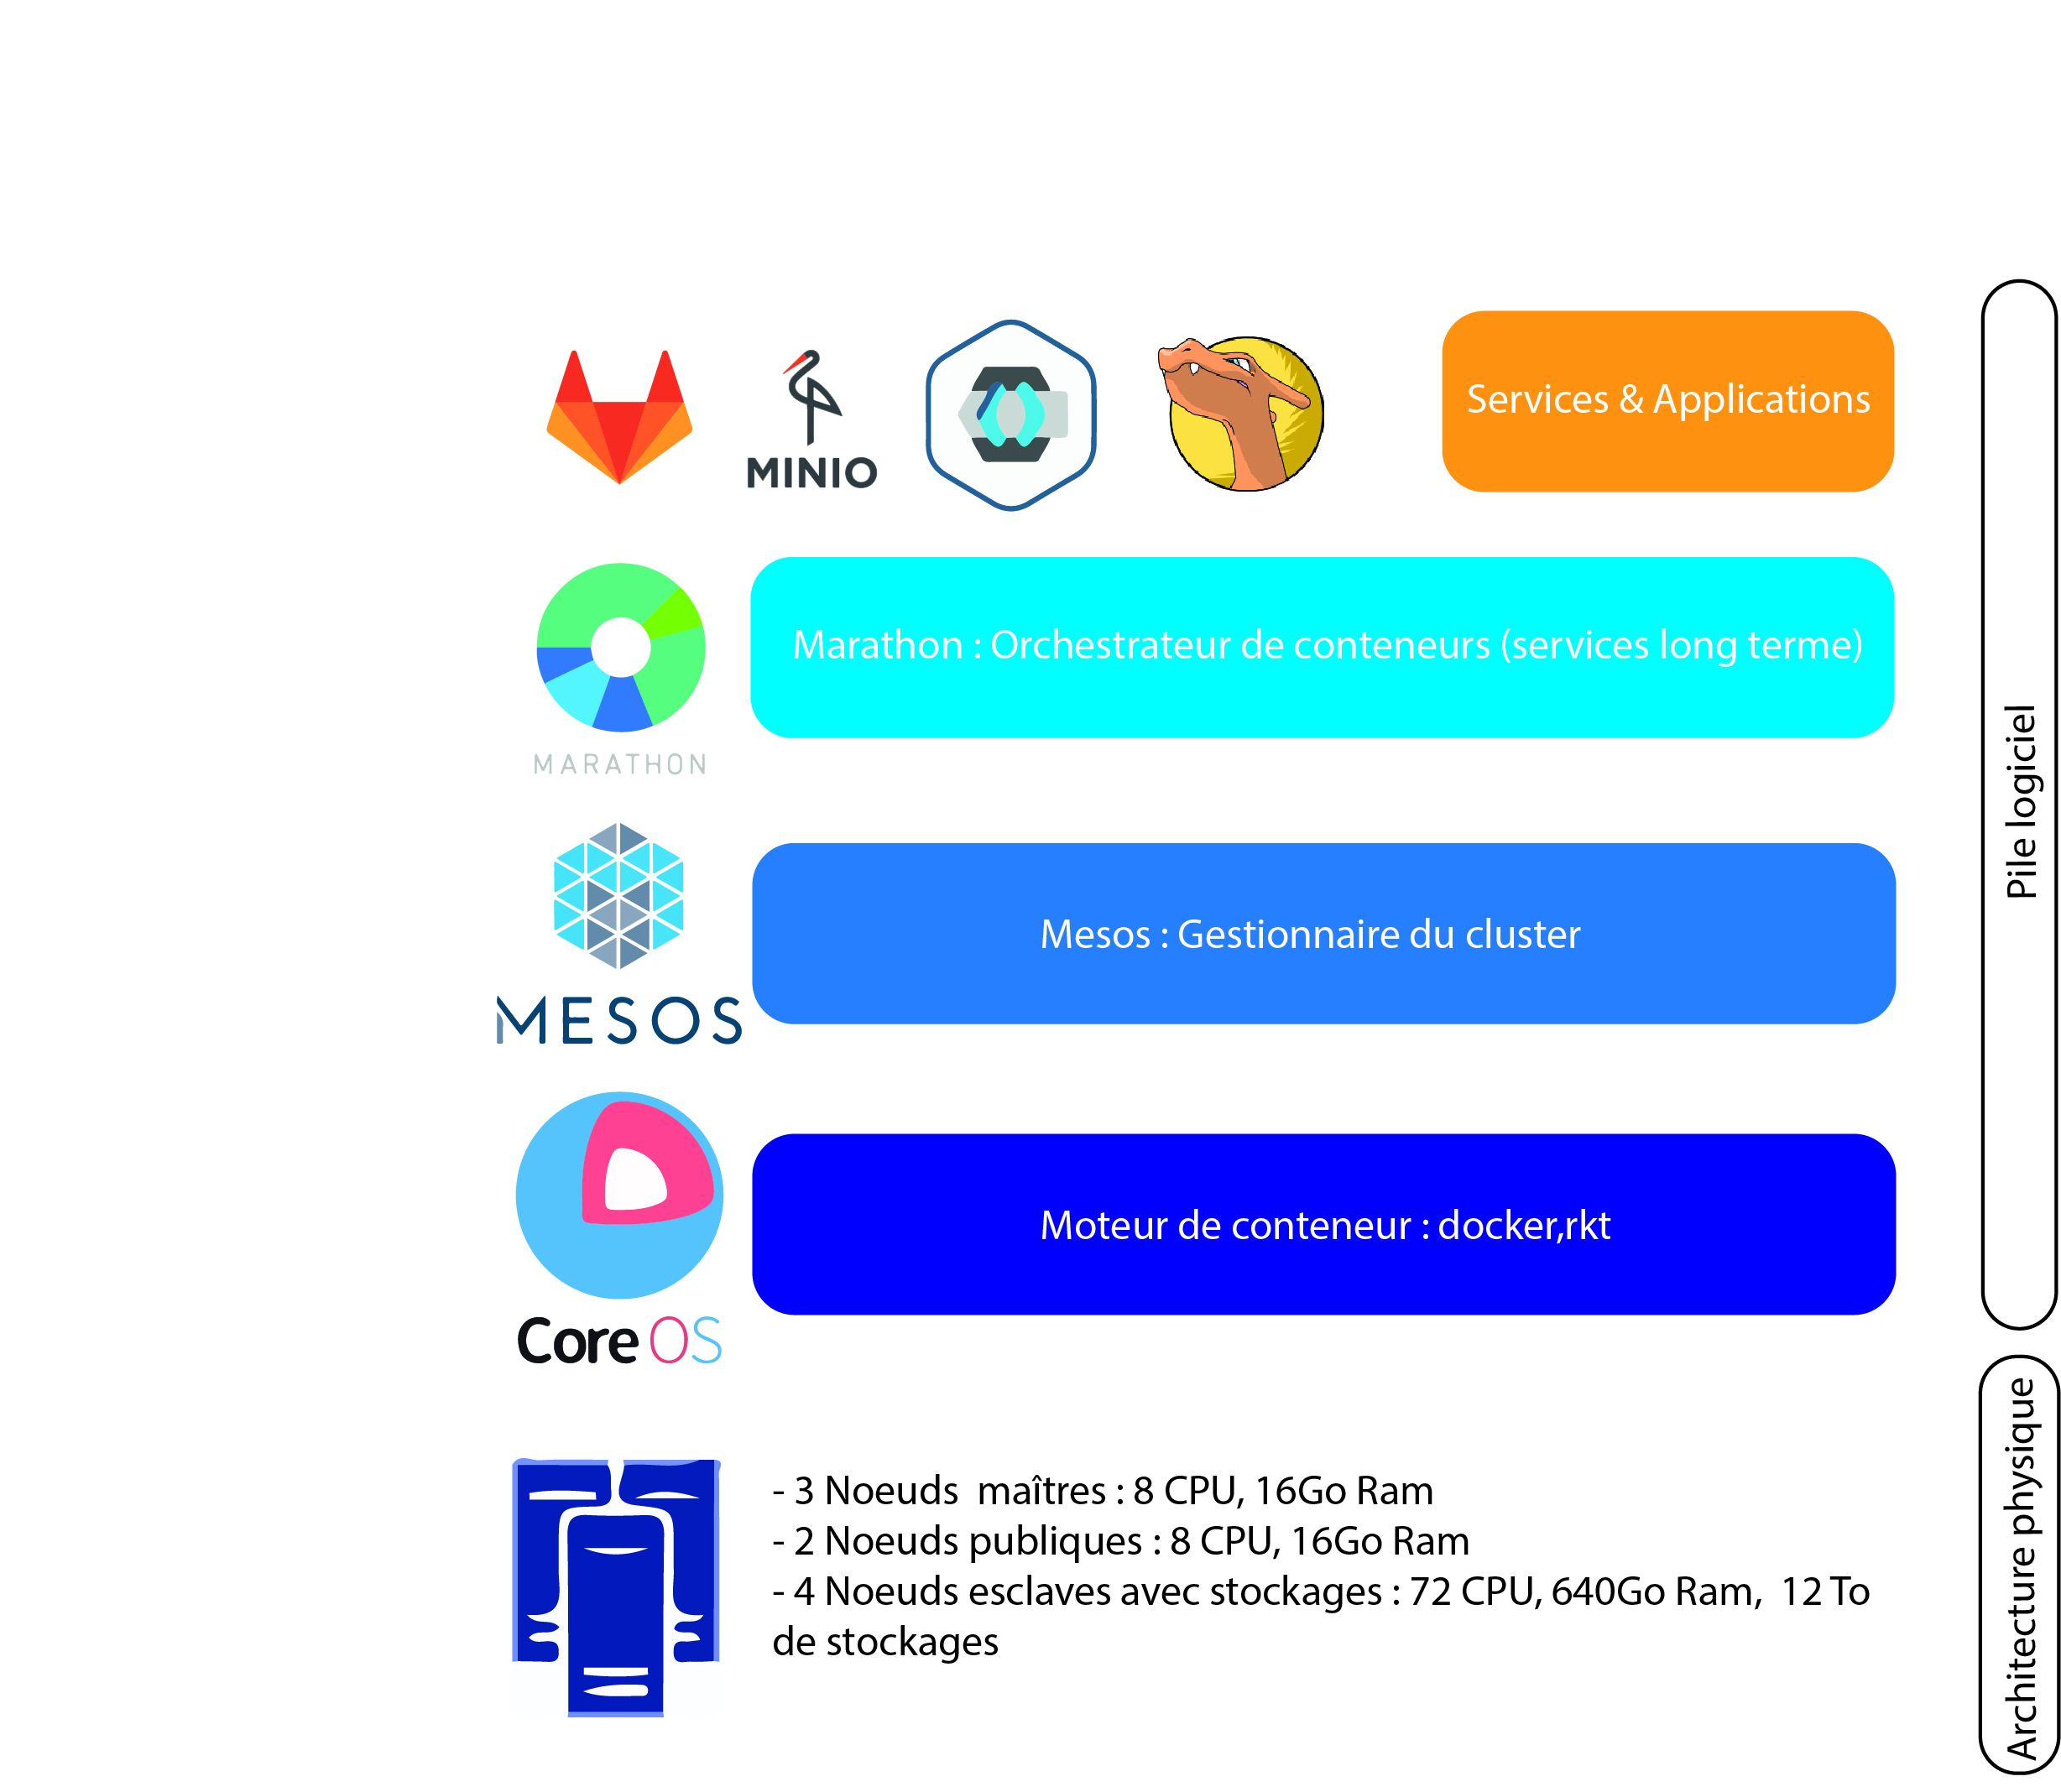
\includegraphics[scale=0.2,clip,trim={18cm, 0cm, 0cm, 11.6cm}]{Pictures/onyxia/Onyxia archi.jpg}
% \captionsetup{margin=1.5cm,format=hang,justification=justified}
% \caption[]{Aperçu simplifié de l'architecture de l'écosystème Onyxia \newline}
% \end{figure}


\section{Objectif et problématique du stage}
Une architecture de type conteneur n'est pas un standard à l'Insee, l'infrastructure de production étant uniquement basée sur des VMs (Virtual Machine ou Machine Virtuelle). L'objectif de mon stage sera donc d'étudier \textbf{les intérêts de la mise en place d'une architecture conteneurisée pour de l'intégration continue ou du service en self-déploiement.}\\

Tout d'abord, nous étudierons les différences entre VM et conteneur afin de comprendre en quoi une architecture conteneurisée peut être un atout. Par la suite, nous verrons qu'une telle architecture se doit de reposer sur un orchestrateur de conteneur. Ce qui nous amènera à faire la comparaison des deux orchestrateurs de conteneurs les plus utilisés actuellement : Marathon (solution utilisée pour la plateforme de l'innovation) et Kubernetes. Pour cela, nous nous appuierons notamment sur ce que les deux orchestrateurs peuvent proposer dans le cadre de l'intégration continue, de services en self-déploiement, ainsi qu'en terme d'aide au développement et de sécurité.


\chapterimage{chapter-image/orchestrateur-01.jpg} % Chapter heading image
\chapter{Orchestrateurs et conteneurs}
\vspace{-2cm}

Dans cette partie nous allons expliquer pourquoi les conteneurs ont été choisi comme brique centrale du datalab. Pour cela, nous repartirons dans le passé et étudierons comment une application était initialement déployée. Nous présenterons également les orchestrateurs de conteneurs, puisque c'est un élément essentiel lorsque l'on doit gérer un parc de conteneurs conséquent.

\section{Du serveur physique au conteneur, évolution}
\subsection{Serveur physique}
Initialement (avant les années 1970 et jusqu'au début des années 2000 à l'Insee), une application était installée sur un un serveur physique. On créait alors les environnements avec des batchs\footnote{Un batch désigne l'automatisation d'une suite de commandes exécutées en série sur un ordinateur, sans qu'il soit nécessaire qu'un opérateur intervienne pour réaliser cette opération.}, que l'on lançait manuellement. Plusieurs applications étaient déployées sur le même OS (Operating System ou système d'exploitation comme Windows par exemple) sur une seule machine physique. On n'avait donc aucun moyen de limiter les ressources utilisées par une application. Par exemple, si sur une machine nous avions deux applications A et B, si A utilisait trop de ressources alors B avait des performances médiocres. La solution aurait été de n'installer qu'une application par serveur, mais cela aurait conduit à des ressources non utilisées et un coût élevé pour les entreprises. \newline


\newline

\subsection{Virtualisation}
Dans un système d'information, plusieurs applications cohabitent et il est nécessaire que les applications soient indépendantes les unes des autres. Les solutions dites de virtualisation permettent de transformer une ressource physique en un ensemble de ressources logiques isolées. Il est donc possible de virtualiser, entre autres, un réseau ou une machine physique. On fait ainsi fonctionner plusieurs “machines” logiques sur une même machine physique appelée hôte. La virtualisation permet de rendre indépendantes les couches basses (matériel) d’une ressource et les couches hautes (applications, traitements). Les couches hautes peuvent ainsi être aisément déplacées sur une autre infrastructure (en cas de panne ou si les ressources deviennent insuffisantes par exemple).
\subsubsection{Les machines virtuelles}
A partir de 1970 (et au début des années 2000 à l'Insee), apparaît  la notion de machine virtuelle (VM). Les VMs sont des serveurs logiques entiers qui embarquent leur propre système d’exploitation. L’hyperviseur est un applicatif tournant sur l’hôte qui va émuler (ou simuler) le matériel pour la machine virtuelle. Le noyau du système d’exploitation de la machine virtuelle croit communiquer avec le matériel de la machine alors qu’il communique avec l’hyperviseur.

Avec le développement des machines virtuelles, de nouveaux outils sont apparus au cours des années 2000/2010 (tels que Puppet\footnote{Puppet est un logiciel libre permettant la gestion de la configuration de serveurs : \url{https://puppet.com/}} ou rundeck \footnote{Rundeck est un logiciel libre permettant l'automatisation d'administration de serveurs via la création de jobs ou tâches : \url{https://www.rundeck.com/open-source}}), qui permettent notamment de configurer automatiquement et rapidement les VMs.


\subsubsection{Les conteneurs}
Un conteneur est une unité logicielle standardisée qui regroupe le code, les dépendances, les binaires\footnote{Les binaires désignent tous les fichiers qui ne sont pas interprétables sous forme de texte. Il peut s'agir de fichier compressé ou exécutable.} et l'environnement nécessaires au bon fonctionnement de l'application. Par conséquent, un conteneur est un "paquet" facile à déplacer d'un environnement à l'autre, puisque tout l'écosystème et tout le code sont présents à l'intérieur de ce conteneur. Un autre avantage est que, peu importe où s'exécute l'application, le fonctionnement sera identique puisque l'écosystème vient avec le conteneur. Cela permet notamment que l'application se comporte de la même façon, à la fois sur le poste du développeur, que sur un cloud privé ou public. \\




\begin{figure}[H]
\renewcommand{\figurename}{Schéma}
\hspace{-1cm}
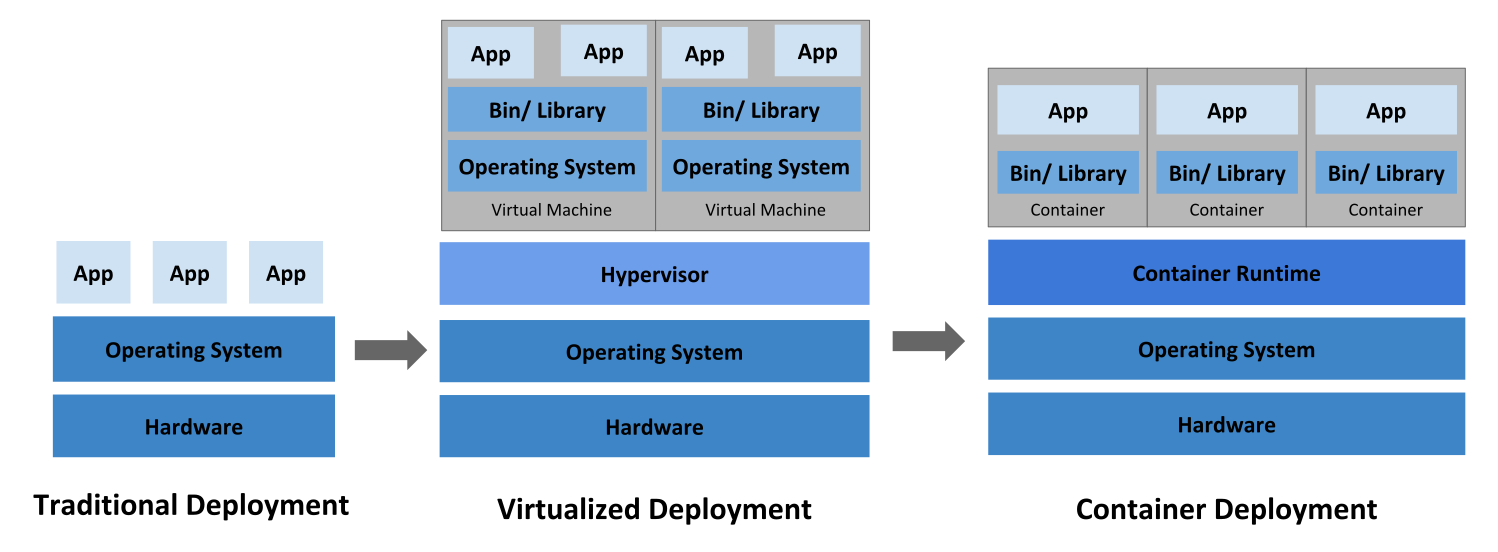
\includegraphics[scale=0.7]{Pictures/container_evolution.png}
\captionsetup{margin=1.5cm,format=hang,justification=justified}
\caption[]{Schéma récapitulatif entre VM et conteneur \newline}
\end{figure}


\section{VM ou conteneur: Lequel choisir en 2020 ? }
Les machines virtuelles comme les conteneurs proposent chacun une solution pour virtualiser des ressources et exécuter des applications. Nous allons aborder ici, divers aspects qu'il faut prendre en compte, avant de s'orienter vers l'une des deux solutions.

\paragraph{Choix du système d'exploitation}
Dans le cadre des VMs, l'administrateur a le choix du système d'exploitation utilisé par chacune des VMs. En effet, chaque VM possède son propre système d'exploitation, il est indépendant des autres OS des VMs installées sur la même machine, et il est même indépendant de l'OS du système hôte. De son coté, le conteneur utilise le système d'exploitation du système sur lequel il est déployé et cet OS est partagé avec l'ensemble des conteneurs qui s'exécutent sur la machine. Les machines virtuelles sont donc plus flexibles sur ce point-ci.

\paragraph{Taille d'une application}
Par ailleurs, cette flexibilité des VMs s'accompagne d'un espace de stockage nécessaire bien plus important. En effet, le "modèle d'une VM" a une taille plus importante que l'image d'un conteneur\footnote{L'image d'un conteneur est un fichier statique non modifiable. Il renferme un code exécutable de manière à exécuter un processus isolé dans une infrastructure informatique.}. Pour une VM, il faut packager le Système d'exploitation, les librairies et l'application. Alors que pour un conteneur, seuls sont nécessaires les librairies et l'application. Ce phénomène s'accentue d'autant plus que l'on veut un nombre de réplicas\footnote{Nombre d'instance d'une application} élevés.

\paragraph{Rapidité de démarrage}
De même, les conteneurs démarrent bien plus rapidement qu'une machine virtuelle.
Selon l'étude \textit{Comparative Study of Virtual Machines and Containers for DevOps Developers\footnote{\url{https://www.researchgate.net/publication/327237114_Comparative_Study_of_Virtual_Machines_and_Containers_for_DevOps_Developers}}}, un serveur web apache (un simple serveur web) met 40 ms pour démarrer et 29 ms pour s'arrêter à partir d'un conteneur, contre près de 59 s pour démarrer et 30 s pour s'éteindre sur une VM.

\paragraph{Rapidité d'écriture des données}
Cette même étude montre également que la vitesse d'écriture et de lecture de données depuis un conteneur est plus rapide que depuis une VM. En effet, un serveur web apache dans un conteneur effectue quasiment autant d'opérations de lecture et d'écriture qu'un serveur web apache installé directement sur une machine. Les VMs ont un rendement 25\% plus faible. 

\paragraph{Sauvegarder, restaurer, migrer}
VirtualBox, VMware ou encore KVM proposent des solutions afin de réaliser des sauvegardes et/ou de restaurer des machines virtuelles à partir de sauvegardes.\\

Dans le monde du conteneur de telles solutions n'existent pas et n'ont pas lieu d'être. En effet le conteneur est une unité qui permet de répondre à un usage précis (traitement) et qui va récupérer les données dans un "volume"\footnote{Espace de stockage rattaché à un conteneur où vont être stockée les données nécessaires à son fonctionnement.}. Dans le monde du conteneur, on cherche donc plutôt à sauvegarder les données que l'état du conteneur.\\  

Des solutions de sauvegarde de l'état d'un conteneur sont quasi inexistantes \footnote{Il existe un projet, en cours de développement appelé CRIU et qui permet de sauvegarder l'état d'un conteneur.}. En effet, une application s'exécutant dans un conteneur n'a pas vocation à vivre éternellement (On verra plus loin que les conteneurs n'ont pas vocation à perdurer (leur durée de vie moyenne étant de 5 min.). Les orchestrateurs de conteneurs peuvent les arrêter et les redémarrer plusieurs fois par jour (et même en production) sans aucune interruption de service.

\paragraph{Sécurité}
Les machines virtuelles offrent une plus grande sécurité. En effet, si un attaquant arrive à sortir de l'application (et à avoir accès à la couche supérieure), dans le cadre d'une VM ce dernier aura accès au BIOS, au réseau de la VM, mais il ne pourra pas accèder aux autres VMs (même celles de la même machine). Les conteneurs n'offrent pas cette isolation, un attaquant qui sortirait de l'application s'exécutant dans le conteneur pourrait alors accéder aux librairies partagées et donc accéder aux autres conteneurs. Cette faille pouvant être causée aussi bien par le développeur que par les dépendances qui auront servies à construire l'image.\footnote{\url{https://www.lemondeinformatique.fr/actualites/lire-une-faille-dans-runc-rend-vulnerable-docker-et-kubernetes-74312.html}} 

\begin{interrupt}
\paragraph{Comment choisir ?}
Dans le cadre de la plateforme innovation et la mise en place de processus d'application en self-service, on recherche une solution de virtualisation qui soit rapide à  déployer, légère, facile à supprimer et à reproduire. Par sa faible taille, le conteneur est également l'outil idéal pour réaliser des tâches d'intégration continue et le déploiement d'environnements de tests à la volée. Les conteneurs semblent donc être la solution idéale, malgré les problèmes de sécurité, puisqu'ils peuvent être facilement contournés (voir annexe \ref{securite}).
\end{interrupt}

\section{Qu'est-ce qu'un orchestrateur ? }
Les architectures applicatives modernes prônent le découpage des applications en modules de petite taille, répondant à un besoin fonctionnel ou technique bien identifié. Ces modules doivent être, dans la mesure du possible, indépendants du système qui les exécute, pour ne conserver que des dépendances logiques entre eux. La notion à la mode est celle d’architecture microservices. Cette notion d'architecture microservices a entrainé une augmentation du nombre de conteneurs déployés afin de faire fonctionner un seul service. Il a donc fallu créer un outil capable de gérer un ensemble de conteneurs : l'orchestrateur de conteneurs.\\ 

La mission d'un orchestrateur de conteneurs est de répartir les conteneurs sur un ensemble de machines. Un orchestrateur de conteneurs est composé de trois ensembles de machines :
\begin{itemize}
    \item Les workers nodes (nœud de travail): ce sont les machines sur lesquels s'exécuteront les conteneurs, ce sont généralement les machines les plus puissantes de la grappe de serveur (cluster). Chacune de ces machines héberge le moteur d'exécution \footnote{Un environnement d'exécution ou runtime est un logiciel responsable de l'exécution des programmes informatiques écrits dans un langage de programmation donné.} ainsi qu'un agent qui communique avec les masters nodes.
    \item Les masters nodes (nœud maître) : ce sont les machines qui vont gouverner le cluster, qui vont gérer l'ensemble des ressources disponibles (RAM, CPU, GPU, espace disque) sur chaque nœud de travail. C'est également le master node qui a la responsabilité de relancer les conteneurs défaillants. C'est généralement le point d'entrée du cluster pour les développeurs.
    \item Les publics nodes (nœuds public) :  ce sont les machines exposées sur internet. Elles vont servir de relais entre internet et l'intérieur de notre plateforme. Ces dernières jouent le rôle de reverse proxy.\\
\end{itemize}
 
L'orchestrateur permet donc d'assurer un rôle de surveillant de l'état des conteneurs. En effet, à partir d'un fichier descriptif qui contient le nombre de conteneurs souhaités, l'état désiré, etc et à l'aide de healtcheck\footnote{Contrôle servant à vérifier si l'application s'exécute correctement} régulier, il est capable de détecter les conteneurs en mauvaise santé. Il pourra ainsi en démarrer de nouveaux et toujours maintenir le système dans un état de fonctionnement optimal.\\
L'orchestrateur est aussi capable de tenir compte des contraintes dynamiques. En effet, les contraintes évoluent dans le temps. Par exemple, on peut vouloir que deux conteneurs ne soient jamais sur le même serveur pour garantir une haute disponibilité de services. Ou encore, on peut vouloir que les conteneurs soient déployés sur des serveurs éloignés afin de limiter la latence pour l'utilisateur. L'orchestrateur sait également réagir en cas de perte d'une des machines. Il permet donc de mettre en place des mécanismes de haut niveau : haute disponibilité, monitoring, Service Discovery \footnote{La découverte de service (ou Service Discovery) est la détection automatique des appareils et services offerts par des appareils sur un réseau informatique}, gestion du trafic réseau,  scalabilité horizontale \footnote{La scalabilité horizontale correspond à l'ajout de nouveaux serveurs réalisant le même type de tâche.} et verticale \footnote{La scalabilité verticale correspond à l'ajout de ressources à un unique serveur (CPU, mémoire, etc).}, provisionning\footnote{En francais provisionnement, désigne l'allocation automatique de ressources.} et placement des conteneurs.\\



\section{Les différents orchestrateurs}
Aujourd'hui, plusieurs solutions d'orchestration existent, mais trois se démarquent : Kubernetes, DC/OS avec Mesos/Marathon et  Docker Swarm.\footnote{Il existe d'autres solutions telles que OpenShift ou encore Rancher mais elles ne sont, au final, que Kubernetes avec un ajout de surcouches.}

\subsection{Mesos/Marathon}
Mesos est la solution la plus ancienne parmi les trois citées. Développée initialement par Mesosphère (qui est devenu DC/OS, puis récemment D2IQ), sa genèse remonte à une époque (2008) où la popularité des conteneurs était nettement moindre. Le concept de Mesos est de regrouper un ensemble de ressources (RAM, CPU) pour proposer une vue agrégée, permettant d’exécuter des programmes (conteneurisés ou pas). Mesos n’a pas vocation à être utilisé seul. Il délègue l’exécution des programmes à ses frameworks\footnote{Voir plus loin}. Parmi eux, les plus utilisés sont certainement Marathon et Aurora. Ce sont eux qui, sur la base d’un fichier de configuration, sont responsables de placer les conteneurs et de garantir leur exécution dans les conditions souhaitées.\\

C'est la solution actuellement utilisée sur la plateforme de l'innovation pour manager les différentes ressources : services à la demande, Gitlab, job Gitlab\footnote{Tâche s'exécutant sur les runners. Un runner est une machine qui sera uniquement réservé pour exécuter des pipelines Gitlab.}, etc... \\ 

\subsection{Kubernetes}
Kubernetes (souvent abrégé k8s) est un produit open source développé initialement par Google, et reversé à la communauté (depuis 2014). Le géant de l’Internet, à l’origine du développement des cgroups\footnote{cgroups (control groups) est une fonctionnalité du noyau Linux pour limiter, compter et isoler l'utilisation des ressources (processeur, mémoire, utilisation disque, etc.).}, utilise les conteneurs depuis près de 15 ans. Le partage de son orchestrateur avec la communauté constitue donc un gage de qualité. \\

Selon Sysdig \footnote{ Rapport disponible ici : \url{https://sysdig.com/blog/sysdig-2019-container-usage-report/}}, plus de 77\% des personnes qui utilisent un orchestrateur de conteneur utilisent Kubernetes. Ce taux monte à plus de 85\% si l'on ajoute les solutions OpenShift et Rancher qui sont basées sur Kubernetes.C'est actuellement l'orchestrateur le plus utilisé dans le monde.\\ 

\begin{figure}[H]\centering
\renewcommand{\figurename}{Graphique}
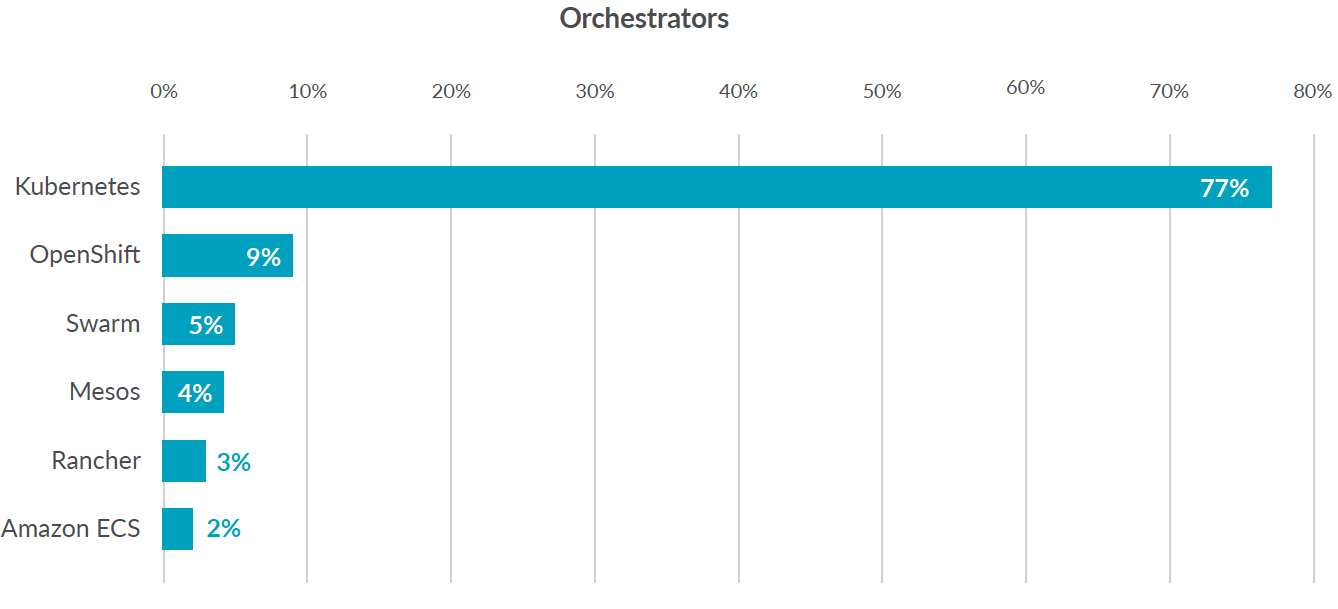
\includegraphics[scale=0.3]{Pictures/orchestrators-2019.png}
\captionsetup{margin=1.5cm,format=hang,justification=justified}
\caption[]{Pourcentage d'utilisation de chaque orchestrateur\newline
Source : Sysdig, \url{https://sysdig.com/blog/sysdig-2019-container-usage-report/}}
\end{figure}

Par ailleurs, Kubernetes bien qu'étant l'orchestrateur de conteneur le plus récent, possède déjà le plus grand nombre de commits\footnote{Un commit est le fait d'enregistrer dans un outil de gestion de versions (GitLab) une nouvelle version d'un ensemble de fichiers.}, une communauté active, et un cycle de développement très court (une version majeure est déployée tous les 3 mois).



\subsection{Swarn Docker}
Swarm est la solution d’orchestration fournie par Docker. Il est difficile de prédire ce que sera Swarm dans un an tant son évolution a été rapide dernièrement. Au départ un composant à part, Swarm est désormais complètement intégré au service Docker. On ne parle plus de Swarm en tant que tel mais du Docker “Swarm mode”.\\


\section{Les solutions retenues}
Pour cette étude, nous nous intéresserons plus particulièrement à Mesos/Marathon (solution actuellement en place à l'Insee sur la plateforme innovation, par le biais de la licence entreprise DC/OS) et Kubernetes. Initialement il était prévu d'expérimenter Kubernetes en interne (par le biais de DC/OS) mais cette solution n'a pas été retenue en bonne partie à cause du confinement. Nous avons donc utilisé Kubernetes par le biais de Google Cloud Provider (GCP)\footnote{Nous avons utiliser GCP pour plusieurs raisons : installer Kubernetes sur ses propres machines est relativement coûteux en temps et en moyen humain (en moyenne, une telle installation nécessite près de 6 mois pour être réalisée par une équipe d'une dizaine de personne à temps plein). La version de Kubernetes proposé par DC/OS était relativement instable. Utiliser GCP nous a permis d'éviter de nous concentrer sur la maintenance des machines et de nous concentrer uniquement sur ce que pouvait apporter l'orchestrateur en terme de fonctionnalités. Ce choix nous a également permis de pouvoir poursuivre les travaux malgré le confinement dû au covid-19.}. Le détail de la mise en place de cette solution est disponible en annexe \ref{Terraform}.\newline



%----------------------------------------------------------------------------------------
%	CHAPTER 2
%----------------------------------------------------------------------------------------
\part{\textcolor{ocre}{\textsc{Mesos vs Kubernetes} : Marathon à bout de souffle ?}}



\chapterimage{chapter-image/deployer-01.jpg} 
\chapter{Architecture et déploiement d'applications}
\vspace{-2cm}
Dans cette partie, nous nous intéresserons aux points communs et différences dans l'architecture des deux orchestrateurs. Nous aborderons ensuite les solutions afin de déployer une application avec l'un ou l'autre des orchestrateurs.

\section{Architecture des deux orchestrateurs}
Le lecteur souhaitant avoir des informations plus techniques et plus complètes sur les deux architectures peut se rendre en annexe \ref{Architecture}.
\subsection{Une architecture commune...}
Kubernetes comme Mesos respectent le design d'architecture d'un orchestrateur de conteneurs classique. On retrouve des worker nodes (appelés "Node" pour k8s et "Mesos Agent" pour Mesos), des master nodes appelés "control-plane" dans les deux cas et des public nodes.\\

Pour les deux orchestrateurs, chaque worker node héberge un environnement d'exécution de conteneur (conteneur-runtime) et un agent qui va remonter l'état des applications déployées ("kubelet" dans Kubernetes, "Mesos Agent" pour Mesos) au master node. Les master nodes sont dans les deux cas composés d'une API\footnote{API signifie Application Programming Interface ou interface de programmation d’application. Une API est accessible par le Web et permet d’établir des connexions entre plusieurs applications pour échanger des données.} permettant au développeur d'exécuter des actions dans le cluster. L'utilisation d'API de type REST est un standard des applications Web modernes.

\subsection{... au fonctionnement différent}
Cependant, Mesos permet l'installation de frameworks. Les frameworks sont des applications que l'on peut ajouter au cluster afin de répondre à certains besoins. Marathon est un de ces frameworks. Il permet au cluster Mesos de réaliser des tâches d'orchestration de conteneurs. Il existe aussi d'autres frameworks tels que Chronos (lancement de tâches) ou encore Aurora.\\

Ces frameworks possédent deux composants : les schedulers et les executors\footnote{Ces composants sont définis en annexe \ref{Architecture}.}. Ces deux composants sont situés respectivement au niveau du control-plane et sur les worker nodes. Chaque Mesos Agent peut être attribué à un ou plusieurs de ses frameworks. Cela vient donc complexifier l'architecture d'un cluster Mesos.\\

Enfin, en pratique on s'aperçoit qu'un cluster Kubernetes peut gérer jusqu'à 5000 nodes, alors qu'un cluster Mesos peut gérer jusqu'à 10 000 Mesos Agents.

\section{Déployer une application : deux approches différentes}
Nous ne présenterons pas ici le code nécéssaire pour le déploiement d'une application (le code de déploiement d'une application dans l'un ou l'autre orchestrateur est présent en annexe \ref{A}), mais les différences entre les deux approches.
\paragraph{Marathon}
 Marathon utilise des fichiers JSON\footnote{JSON (JavaScript Object Notation) est un format de fichier dérivé de la notation des objets du langage JavaScript. Comme XML, ce format permet de représenter de l’information structurée.} pour la configuration des déploiements. La configuration du déploiement s'effectue par l'intermédiaire d'un seul fichier. Dans ce fichier, on retrouve notamment : l'image que l'on veut utiliser, l'URL sur laquelle le service sera rendu accessible, les variables d'environnements qui seront par la suite injectées dans le conteneur, le nombre de réplicas, la limitation de CPU et/ou de mémoire. On peut également, lors du déploiement du service, télécharger au préalable un ou plusieurs fichiers et les ajouter directement au conteneur. L'envoi de ce fichier à Marathon se fait par l'intermédiaire d'une requête POST\footnote{Une requête POST est une requête WEB permettant d'envoyer du contenu à un serveur.} ou de la CLI\footnote{CLI signifie Command Line Interface (en français, interface en ligne de commande).} DC/OS.
 
\paragraph{Kubernetes}
Kubernetes utilise des fichiers YAML\footnote{YAML (Yet Another Markup Language) est un format de représentation de données.} pour la configuration des déploiements. Le déploiement d'une application se fait par l'assemblage de plusieurs fichiers (qui sont en fait la description de ressources). Lors d'un déploiement, l'utilisateur doit configurer au moins trois objets k8s (par le biais de trois fichiers ou manifestes) : l'objet deployement (déploiement), l'objet service et l'objet ingress. Le premier sert à créer un ensemble de Pods \footnote{Un Pod est la plus petite unité logique de k8s. Il encapsule un conteneur applicatif. Un Pod est attaché à un node, son existence est temporaire, on peut facilement le répliquer sur un autre node. Chaque Pod a une adresse IP virtuelle unique au sein du cluster, ce qui permettra aux autres Pods du cluster de communiquer avec ce dernier.} dans notre cluster, ce Pod est situé sur un des nodes, mais il n'est pas accessible (ni de l'intérieur ni de l'extérieur du cluster). Le service \footnote{Un service peut être défini comme un ensemble logique de Pods exposés en tant que service réseau. C'est un niveau d'abstraction au-dessus du Pod, qui fournit une adresse IP et un nom DNS unique pour un ensemble de Pods.} va permettre d'exposer à l'intérieur du cluster ce Pod. Enfin, l'ingress permettra d'exposer ce service au monde extérieur. Cette séparation par objet est à la base de Kubernetes. Par exemple, l'ajout de variables d'environnement passe par l'intermédiaire d'un autre objet : les configMaps.\\

Kubernetes rajoute la notion d'init-container, c'est un container s'exécutant avant celui que l'on veut déployer et qui va permettre de réaliser des actions : téléchargement de données, tests de connexion à certains outils... \newline


Enfin, Kubernetes permet l'isolation des ressources entre divers utilisateurs, par l'intermédiaire des namespaces. Un namespace est une partition virtuel du cluster Kubernetes. C’est un moyen de diviser un cluster Kubernetes entre plusieurs utilisateurs. Deux ressources au sein du même namespace ne peuvent pas avoir le même nom, mais entre deux namespaces oui. Sauf mention contraire, une ressource d’un namespace ne peut aller interroger directement une ressource d’un autre namespace, cela permet d’isoler les déploiements d’un groupe d’utilisateurs.

La communication avec le cluster k8s, notamment pour l'envoi des fichiers de configurations à l'orchestrateur, se fait par l'intermédiaire de la CLI kubectl. Cette ligne de commande communique directement avec l'API du cluster. C'est le moyen à privilégier pour communiquer avec le cluster bien que certaines librairies java communiquent directement avec l'API sans passer par la CLI kubectl.

\begin{figure}[H]\centering
\begin{tabular}{@{}lll@{}}
\toprule
                             & Marathon       & Kubernetes      \\ \midrule
Fichiers/déploiement         & un seul         & Plusieurs       \\
Language                     & JSON           & YAML            \\
Isolation entre utilisateur & Oui (mais avec de la configuration)            & Oui nativement (namespace) \\
Variable d'environnements    & Balise env     & ConfigMap       \\
Télechargement de ressources & Balise Fetch   & InitContainer   \\
Stockage                     & Balise Stockage & VolumeClaim     \\
Communiquer & DC/OS CLI, API, Marathon UI & kubectl CLI, API\\
\bottomrule
\end{tabular}
\caption{Tableau Récapitulatif des fonctionnalités communes et différentes entre Marathon et Kubernetes dans le cadre du déploiement d'une application}
\label{tab:my-table}
\end{figure}


\begin{interrupt}
\paragraph{Conclusion :}
Le déploiement d'une application est donc bien plus verbeux dans Kubernetes que dans le cadre de Marathon. Mais la contrepartie est que cela permet une plus grande finesse dans la configuration des déploiements. Un exemple complet de code permettant de déployer une application dans le cadre des deux orchestrateurs se trouve en annexe \ref{A}.
\end{interrupt}

\section{Des outils d'aide au développement}
Le développeur peut également être intéressé par les outils d'aide au développement qui accompagnent chaque orchestrateur. En effet, un orchestrateur est attractif si il est simple de développer, de débugger et d'y surveiller les applications.\\

Avec Marathon, les outils mis à la disposition du développeur sont peu nombreux. En effet, la ligne de commande DC/OS permet uniquement de déployer une application. L'interface administrateur de DC/OS permet de suivre l'état du cluster, la consommation de chaque node, la gestion des alertes, etc. Par l'intermédiaire de l'interface graphique (ou de la CLI) de Marathon, le développeur peut consulter les logs d'exécution de ses déploiements. La CLI Mesos permet également d'exécuter directement du code dans un conteneur, ce qui peut être utile pour débugger. Mais pour cela il faut configurer la CLI de Mesos, ce qui n'est pas évident et la gestion des droits n'est pas aisée non plus. C'est d'ailleurs pour cette raison que l'innovation possède deux Marathons. Le premier est dédié au développeur dans le cadre de l'intégration continue, le deuxième est réservé au déploiement d'application "stable" tel que gitlab, rocketchat, etc. \\

Kubernetes propose lui aussi toutes ces fonctionnalités. L'équivalent de l'interface administrateur est le Kubernetes dashboard. Mais puisque les identifiants de connexions sont des tokens\footnote{Jeton d'authentification fourni à l'API pour s'authentifier. Le token comporte est généralement hashé et comporte des informations concernant l'utilisateur, ainsi qu'une clés servant à l'authentification.} Kubernetes, le dashboard permet également la restriction de ressources et/ou de namespaces. La CLI kubectl apporte de nombreuses autres possibilités de lister l'ensemble des ressources déployées, d'en créer de nouvelles etc... IL possède également une fonctionnalité permettant de "port-forward" un Pod: Grâce à cette fonctionnalité, le développeur peut accéder à son Pod directement depuis son poste et sans avoir à configurer d'autres objets. La CLI kubectl permet également de faire des retours arrières sur nos déploiements, d'accéder directement aux objets déployés dans le cluster et de les modifier avec un éditeur intégré. Par ailleurs, de nombreuses extensions existent, comme l'extension VScode Kubernetes qui détecte automatiquement la configuration Kubernetes présente sur notre poste. Cela permet notamment de rassembler l'ensemble des outils du développeur au même endroit. Cette extension permet également de générer des squelettes d'objets deployment, service, ingress, etc. Il existe aussi l'outil Lens qui est un IDE\footnote{IDE signifie Environnement de Développement Intégré.} pour Kubernetes \footnote{voir ici : \url{
https://github.com/lensapp/lens}}.

\section{Du template au gestionnaire de paquets}
Il arrive que certaines applications soient déployées dans des environnements différents (par exemple dev, qf, prod, etc.). Plutôt que d'écrire plusieurs fois les même fichiers de configuration en modifiant seulement certains paramètres, il peut être intéressant de bénéficier d'un squelette de l'application qui sera ensuite adaptable à chacune des plateformes.
\subsection{Des formats de templatings}
Kubernetes, par le biais de l'outil "Kustomize", permet de définir des templates d'application. Cet outil fonctionne de la manière suivante :
\begin{itemize}
    \item on dispose des fichiers décrivant un déploiement de l'application avec des paramètres par défaut.
    \item un fichier nommé "kustomize.yaml"  fait référence aux fichiers précédents et va redéfinir certaines variables contenues dans ces fichiers.
    Déployer dans différents environnements revient donc à créer un fichier "kustomize" par environnement.
\end{itemize}
Ce n'est pas le seul outil de création de modèle d'application existant dans Kubernetes : on citera notamment "jsonnet" et "ksonnet", non utilisés au cours de ce stage.\\ 

DC/OS, quant à lui, a introduit la notion de Universe pour Mesos/Marathon. Les Universes utilisent le moteur de template Mustache. 
Ce format de templates fonctionne à l’aide de “tags”, représentés sous la forme suivante : \{\{variableName\}\}. (Les accolades représentent les fameuses moustaches.) On possède donc un modèle d'application avec ces tags aux endroits que l'on souhaite modifier. On utilise ensuite manuellement un outil permettant, à partir d'un objet de configuration, de remplir ces "trous". Ce format n'a pas vocation a être utilisé manuellement. En effet, c'est un outil intermédiaire dans la mise en place d'un gestionnaire de paquets pour Mesos/Marathon par DC/OS.


\subsection{Des gestionnaires de paquets}
Le principe d'un gestionnaire de paquets est de pouvoir faciliter le déploiement d'un service au sein d'un environnement. Par exemple, si je veux installer wget sur Linux, il suffit d'ouvrir un terminal et taper \textit{sudo apt-get install wget}. Il pourrait donc être intéressant de disposer du même type d'outils mais au sein d'un cluster. Cela permettrait, par exemple, de pouvoir installer rapidement des applications telles que Keycloak (authentification), la sphère Prometheus-Grafana, ou encore la brique ELasticSearch et Kibana (ELK). Marathon comme Kubernetes proposent chacun leur gestionnaire de paquet. Helm pour Kubernetes, Universe pour DC/OS. \\

Universe n'est pas directement un gestionnaire de paquets, mais un format de templating développé afin d'être utilisé par le gestionnaire de paquets de DC/OS. Ce gestionnaire de paquets est accessible depuis l'interface graphique de DC/OS ou depuis la CLI DC/OS. Par défaut, DC/OS propose 120 applications installables par le biais de ce gestionnaire de paquets. Pour plus d'informations sur le fonctionnement des Universes, le lecteur peut se rendre en annexe \ref{Universe}. \newline 

Helm, quant à lui, est une CLI qui permet à la fois de déployer des paquets (appelé charts) dans Kubernetes, mais aussi de lister les services déjà installés, de réaliser des montées de versions, de créer de nouveaux paquets, et d'ajouter de nouveaux répertoires contenant d'autres paquets. Et, comme Universe, c'est aussi un outil qui fournit son propre format de templating.\newline

Par ailleurs, Helm est le gestionnaire de paquets recommandé par la Cloud Native Computing Foundation pour Kubernetes, ce qui lui vaut un certain succès. En effet, Helm propose plus de 1200 Charts Helm (bien loin des 120 paquets du répertoire DC/OS) qui sont référencés sur \url{https://hub.helm.sh/}. Ce hub\footnote{Plateforme regroupant l'ensemble des ressources sur un sujet précis au même endroit. Ici on cette plateforme regroupe l'ensemble des charts Helm} contient l'ensemble des Charts Helm considérés comme stables par Google. Mais il existe aussi de nombreux répertoires Helm alternatifs. Plus d'informations sur le fonctionnement de Helm est disponible en annexe \ref{Helm}.\newline








\chapterimage{chapter-image/git-01.jpg} 
\chapter{CI/CD: Kubernetes un pas vers le GitOps}
\vspace{-2cm}
L'intégration continue (CI) et le déploiement continu (CD) permettent de rapprocher les Dev. et les Ops. En effet, les Dev. et les Ops. ont des objectifs différents. Les premiers voudraient être libres de déployer leur code, bien souvent basé sur les dernières technologies à la mode. Les seconds gèrent les plateformes en contraignant, parfois, toutes formes de nouveauté. Le DevOps est né de cette impérieuse nécessité de réduire ce profond clivage. Puisque la plupart des entreprises ont adopté Git comme outil de gestion de code, on parle désormais de pratique GitOps. Dans ce chapitre, nous définirons le GitOps, et nous verrons si son utilisation est compatible avec l'un ou l'autre des deux orchestrateurs étudiés.

\section{GitOps: tout est "code-centric"}
Le GitOps est une approche où on décrit l’état souhaité de notre infrastructure dans Git. Un opérateur (une application intermédiaire) surveille le répertoire, et si des modifications ont lieu, il applique les changements nécessaires pour s’assurer que l'état actuel (l’état de l’environnement) tendent toujours vers l’état souhaité (le contenu du répertoire). 

\begin{figure}[H]\centering
\renewcommand{\figurename}{Schéma}

\includegraphics[scale=0.8]{Pictures/CI-CD/gitops-Intro.png}
\captionsetup{margin=1.5cm,format=hang,justification=justified}
\caption[]{Schéma simplifié du fonctionnement de GitOps \newline}
\end{figure}

Les changements via l’interface utilisateur sont limités au maximum. Tout changement doit être approuvé par le biais de merge requests\footnote{Une merge request désigne une demande de fusion entre le code nouvellement développé et le code déjà présent sur le répertoire Git.}. Suite à cette approbation, la modification sera appliquée automatiquement par l’opérateur.\\

On retrouve deux modèles pour implémenter le GitOps: le modèle en push et le modèle en pull. Les deux modèles reposent sur la présence de deux répertoires Git : le premier contenant le code de l'application, le second contenant les fichiers pour le déploiement. Les étapes suivantes ont lieu dans les deux modèles : 
\begin{itemize}
     \item Un nouveau commit déclenche le pipeline de compilation de l'application (appelée "build"). Ce pipeline de build compile l'application puis lance les tests.
    \item Si les tests passent, alors on construit l'image docker associée à l'application puis on la push\footnote{Push, dans le cadre d'un outil de gestion de version comme Git, signifie envoyer les modifications du répertoire local au répertoire distant (Git).} sur le répertoire d'image.
    \item Enfin, le pipeline de CI se termine en pushant sur le répertoire contenant la configuration, la nouvelle version de l'image à utiliser.
\end{itemize}
C'est par la suite que l'on distingue le modèle en push du modèle en pull.

\subsection{Le modèle en push}
\begin{figure}[H]
\renewcommand{\figurename}{Schéma}
\hspace{-1cm}
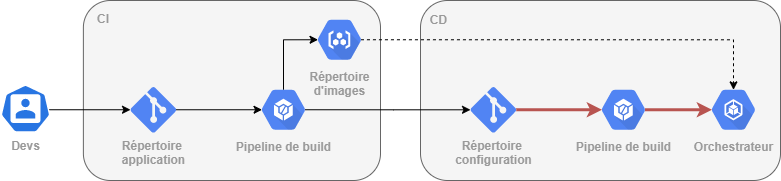
\includegraphics[scale=0.6]{Pictures/CI-CD/push-model.png}
\captionsetup{margin=1.5cm,format=hang,justification=justified}
\caption[]{Schéma simplifié du modèle push de GitOps \newline}
\end{figure}

Dans le modèle en push, lorsque le répertoire contenant la configuration est mis à jour, un nouveau pipeline se lance afin d'envoyer la nouvelle configuration vers l'orchestrateur.\\

L'application qui envoie (push) les changements vers l'orchestrateur joue alors le rôle de l'opérateur. Avec ce modèle, on ne peut cependant pas distinguer (sans monitoring ou investigation manuelle) une divergence entre la version s'exécutant dans le cluster et la version du répértoire git. 

\subsection{Le modèle en pull}
\begin{figure}[H]
\renewcommand{\figurename}{Schéma}
\hspace{-1cm}
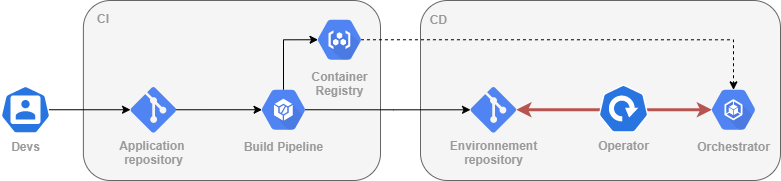
\includegraphics[scale=0.6]{Pictures/CI-CD/pull-model.png}
\captionsetup{margin=1.5cm,format=hang,justification=justified}
\caption[]{Schéma simplifié du modèle pull de GitOps \newline}
\end{figure}

Dans le cadre du modèle en pull, un opérateur surveille en continue le répertoire contenant la configuration de l'application. Cet opérateur détecte alors une différence entre l'état souhaité et l'état courant. Il récupère l'état souhaité (pull), Il applique alors un patch\footnote{un correctif} afin de rétablir l'état du cluster vers celui du répertoire Git. Ainsi, si une opération est faite manuellement directement dans le cluster, l'opérateur va remettre en conformité l'état du cluster avec l'état souhaité.

\section{Pourquoi choisir d'utiliser des pratiques GitOps ? }
\begin{itemize}
    \item Le répertoire Git contient l'historique des modifications. Cela permet de voir comment l'infrastructure a évolué. Les messages de commits s'ajoutent à la documentation déjà existante. De plus, cela permet de voir le déploiement comme du code. On peut donc désormais pratiquer les techniques de "pair programming"\footnote{Le pair programming est une technique de développement logiciel agile dans laquelle deux programmeurs travaillent ensemble sur un même poste de travail. L'un, le driver, écrit le code tandis que l'autre, l'observateur, examine chaque ligne de code au fur et à mesure qu'elle est tapée. Les deux programmeurs changent fréquemment de rôle
} ou d'"extreme programming"\footnote{Méthode de développement d'application consistant à développer une application par sprint très court.} qui ne peuvent être que bénéfiques. En effet, ces pratiques apportent beaucoup sur la qualité de code et de partage de connaissances sur le projet.
    \item Les tickets kanboard \footnote{Dans le développement de logiciel, un système Kanban  est utilisé afin de limiter les tâches-en-cours. Ce système s'appuie sur les tickets kanboard. Un ticket Kanboard représente une tache à effectuer.} n'ont plus de raison d'être et sont remplacés par des merges request. La merge request explique les besoins et le propriétaire du dépôt vérifie la validité de la merge request et l'accepte (ou non). On a donc deux avantages :  une réduction des erreurs humaines et un partage de connaissances.
    \item Revenir en arrière suite à un déploiement, revient simplement à annuler la dernière fusion (faire un git revert sur le dernier commit).
    \item Comme tous les changements passent par Git, les modifications sont auditables. De plus, avec le  modèle en pull, seul l’opérateur a le droit de déployer dans le cluster. Il n'y a donc plus besoin de stocker les identifiants du cluster dans GitLab pour le CI. On a donc moins d'identifiants d'accès au cluster stockés à divers endroits, on limite ainsi les problèmes de sécurité.
\end{itemize}




\section{Quels outils choisir ?}
\paragraph{GitLab CI}
L'outil GitLab CI permet de faire du « CD » (déploiement continu) dans le cadre de la stratégie « push ». \\

C’est d'ailleurs la solution actuellement utilisée à l'Insee. En effet, les équipes qui souhaitent faire du CD, mettent en place en fin de pipeline un job qui sera en charge de déployer la nouvelle application. Pour une utilisation avec Marathon ou Kubernetes, on peut par exemple avoir un dossier dans notre projet contenant des templates de fichiers de déploiements qui seront remplis par une tâche en fin de pipeline \footnote{Cette solution est celle actuellement utilisée à l'Insee avec Marathon. Un exemple d'implémentation est disponible ici: \url{www.gitlab.com/Donatien26/demo-ci}.}. Cette solution trouve notamment son intérêt dans le cadre de déploiement d'environnements de tests, pour par exemple valider des demandes de fusions. En effet, redéployer une application nécessite de relancer tout le pipeline.\\

\begin{figure}[H]\centering
\renewcommand{\figurename}{Schéma}
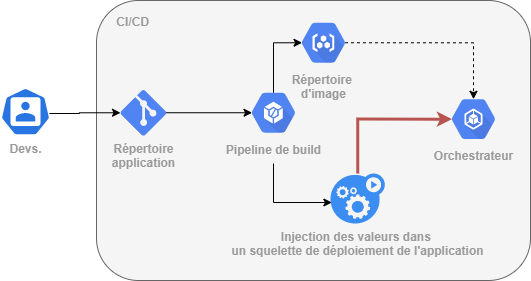
\includegraphics[scale=0.55]{Pictures/CI-CD/insee-model.png}
\captionsetup{margin=1.5cm,format=hang,justification=justified}
\caption[]{Modèle Push actuellement utilisé à l'Insee \newline}
\end{figure}

Par ailleurs, GitLab propose également une intégration avec des clusters Kubernetes. Il suffit d’ajouter au projet GitLab les identifiants requis pour se connecter au cluster Kubernetes en question, pour que ce dernier déploie directement dans Kubernetes.\footnote{\url{https://docs.gitlab.com/ee/user/project/clusters/}}


\paragraph{Flux}
Flux est l’outil de CD de Weave\footnote{Un projet CNCF classé en tant que « Sandbox Project »}. Flux repose sur le modèle en pull. Il utilise un opérateur dans le cluster pour déclencher des déploiements à l'intérieur de Kubernetes. En plus de surveiller les dépôts Git, il est également capable de surveiller des dépôts d'images docker, d'y détecter les nouvelles images utilisées, et en fonction de règles définies au préalable il peut déclencher, ou non, la mise à jour des applications déployées dans le cluster.

\paragraph{Argo CD}
Comme Flux, Argo CD est un opérateur Kubernetes synchronisant l'état de l'application dans le cluster avec la description des fichiers Kubernetes stockés dans un dépôt Git. Il s’inscrit lui aussi dans le modèle en pull. Argo CD est capable de surveiller un répertoire d'images (depuis début août). Mais contrairement à Flux, il dispose d'une interface et d'une CLI que le développeur peut utiliser pour créer et suivre les ressources d’Argo CD (pour plus d'informations voir sous partie suivante).

\paragraph{Dispatch}
Dispatch est un outil payant proposé par D2IQ (anciennement DC/OS) dans le cadre de son offre Kubernetes. Il s'appuie sur deux outils : Argo et Tekton. Il permet de décrire des pipelines Tekton et de générer automatiquement les configurations Argo. Il repose donc sur le modèle en pull.

\paragraph{Argo Flux}
Argo Flux est un projet très récent, annoncé peu avant la KubeCon 2019 (Conférence annuel sur l'ensemble des technologies gravitant autour de Kubernetes). Il a pour ambition d’être la fusion des projets Argo CD et Flux. Weave, Intuit et AWS ont annoncé collaborer ensemble sur le projet  \footnote{https://www.weave.works/blog/argo-flux-join-forces} et vont participer à son développement. Le projet n'a pour l'instant aucune version testable.

\begin{interrupt}
\paragraph{Remarque}
Les solutions ci-dessus sont majoritairement orientées Kubernetes. En effet, il n'existe pas de solution orientée DevOps (ou GitOps) dans Marathon. C'est d'ailleurs une des raisons qui pousse les entreprises à utiliser Kubernetes comme orchestrateur de conteneurs. Marathon ayant été conçu avant que les notions de GitOps ne deviennent une généralité.
\end{interrupt}
\section{Argo: Vers une architecture conteneurisée en production}

ArgoCD suit le modèle en pull GitOps, qui consiste à utiliser les dépôts Git comme source de vérité pour définir l'état d'application souhaité. C'est un projet relativement jeune (lancé en 2017) mais qui fait parti des outils recommandés par la CNCF dans sa carte de route pour concevoir une plateforme cloud \footnote{\url{https://github.com/cncf/trailmap/blob/master/CNCF_TrailMap_latest.pdf}}. C'est également l'outil utilisé par le Ministère de l'Intérieur pour la mise en place de sa plateforme cloud.  ArgoCD possède son Chart Helm qui lui permet d'être facilement déployable dans Kubernetes et il ne fonctionne qu'avec des ressources Kubernetes. ArgoCD a été choisi pour la plateforme de l'innovation car il permet notamment l'authentification OIDC\footnote{Authentification de type open-id connect, authentification à jeton}, la gestion de droits et il propose une interface graphique. \newline

ArgoCD permet d'automatiser le déploiement d'applications dans les environnements cibles spécifiés. ArgoCD est un contrôleur Kubernetes qui surveille en permanence les applications fonctionnant dans le cluster. Il les compare à l'état défini dans le dépôt Git. S'il détecte une déviation, il marque une application comme étant "OutOfSync"\footnote{Perte de la synchronisation} (indiquant que le cluster ne reflète pas actuellement la branche master du dépôt) et le cas échéant il la resynchronise avec le répertoire Git.  ArgoCD est compatible avec plusieurs types de manifestes \footnote{Un manifeste est un fichier JSON ou YAML qui permet de déclarer le type d'application à exécuter et le nombre de réplicas nécessaires pour exécuter un système sain.} Kubernetes: des templates d'application avec Kustomize, des Charts Helm, des applications ksonnet, des fichiers Jsonnet, ou encore directement des fichiers YAML.\newline



ArgoCD propose plusieurs moyens pour communiquer avec lui : une interface, une ligne de commande (ArgoCD), il expose également une API compatible REST et gRPC\footnote{gRPC est un framework RPC (Remote procedure call) open source initialement développé par Google. Le RPC est un protocole réseau permettant de faire des appels de procédures sur un ordinateur distant à l'aide d'un serveur d'applications.}. Il peut, dans le cas où l'on souhaite réduire le temps entre chaque synchronisation du répertoire Git, être configuré pour recevoir des notifications Git. Par ailleurs, ArgoCD peut envoyer des notifications dans d'autres applications telles que Slack (pour avertir d'une montée de version ou qu'une application n'est plus synchronisée par exemple). Il est également capable de gérer l'état des applications dans plusieurs clusters Kubernetes en étant déployé dans un seul cluster.
L'interface graphique d'ArgoCD permet notamment d'avoir une vue explosée de nos déploiements. Sur la capture d'écran~\ref{onyxia-argo} de l'exemple du déploiement d'Onyxia, on retrouve toutes les entités de Kubernetes : ingress, Pod, deployment, Service, role-binding,... On a également accès aux manisfestes, logs de chaque composant, historique de déploiement, ainsi que la possibilité de faire des rollbacks\footnote{Un rollback est un retour sur une version précédente de l'application.} en un clic.

\begin{figure}[H]
\renewcommand{\figurename}{Schéma}
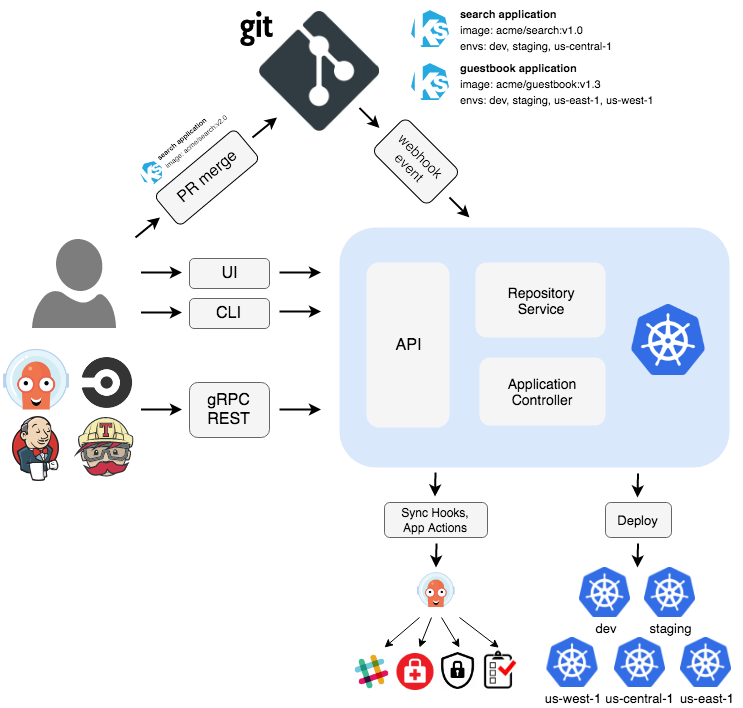
\includegraphics[scale=0.1]{Pictures/CI-CD/argocd_architecture.png}
\captionsetup{margin=1.5cm,format=hang,justification=justified}
\caption[]{Architecture et fonctionnement de l'environnement Argo \newline}
\end{figure}

\begin{figure}[H]
\renewcommand{\figurename}{Capture d'écran}
\hspace{-2.5cm}
\includegraphics[scale=0.5,trim={0 0 5cm 0},clip]{Pictures/CI-CD/Onyxia-argo.PNG}
\captionsetup{margin=1.5cm,format=hang,justification=justified}
\caption[]{Déploiement de Onyxia dans Argo \newline}
\label{onyxia-argo}
\end{figure}
 


\section{Le GitOps: oui mais pour quel projet ?}
Avant de se lancer dans le GitOps, il faut d'abord que notre projet réponde à certains critères. En effet, les problèmes les plus fréquents dans un cluster sont les suivants: \\
\begin{itemize}
    \item Le downtime : Si un conteneur (ou pire un worker node) contenant une application dysfonctionne pour une raison quelconque, il faut que l'orchestrateur relance cette application. Durant ce laps de temps, l'application peut être indisponible. On parle alors de downtime. Un moyen de palier à ce problème est d'avoir plusieurs répliques de notre application réparties sur plusieurs nodes, pour qu'en cas de bug d'une des répliques, les autres prennent le relais. Il est donc interdit à l'application de posséder des données en local. \\
    
    \item La surcharge : Il peut arriver que le cluster soit en surcharge suite à une trop forte demande des utilisateurs, ou encore suite la perte d'un node obligeant le déplacement des applications sur un autre node (perte de ressources entraînant une surcharge). Une surcharge peut également avoir lieu lorsque l'ensemble des  applications consomme toutes les ressources disponibles. Pour cela on a deux solutions : prévoir large (c'est-à-dire surdimensionner le cluster, mais cela entraîne une non utilisation des ressources) ou bien faire de l'autoscaling (littéralement mise à l'échelle automatique, c'est-à-dire laisser automatiquement le cluster démarrer des worker-nodes ou des conteneurs afin de répondre à la charge, le problème est que cela peut être coûteux). \footnote{C'est d'ailleurs à cause de cette raison que Amazon s'est initialement converti en fournisseur cloud : leur serveur était surchargé pendant certaines périodes de l'année (fêtes de fin d'année). Ils ont donc décidé de louer les ressources qu'ils n'utilisaient pas le reste de l'année, afin de rentabiliser leur infrastructure.} Dans tout les cas l'application se doit donc d'être scalable\footnote{(littéralement mise à l'échelle) Une application est dite scalable si elle possède la capacité à maintenir ses fonctionnalités et ses performances en cas de forte demande (montée en charge). Elle doit être scalable verticalement (augmentation des ressources allouées :  CPU, mémoire...) et scalable horizontalement (augmentation du nombre de répliques de l'application), le premier étant plus facile à garantir que le second.}.\\

    \item La perte de donnée : de la même façon que précédemment, aucune donnée ne doit être attachée à un conteneur. Il faut donc, dans le cas du stockage de données (comme pour une base de données par exemple), avoir une certaine redondance des données et/ou pouvoir les externaliser. Les applications stateless\footnote{(ou sans état) Désigne une application qui ne sauvegarde pas les données de l'utilisateur générées lors d'une session pour les utiliser lors de la session suivante avec cet utilisateur} ne possèdent aucune donnée en local, tout leur état étant déporté sur une autre application.\\
\end{itemize}

On a alors besoin d'avoir des applications cloud-Native. La CNCF donne la définition suivante du cloud-native: \\

\textit{"Les technologies cloud-native permettent aux entreprises de construire et d'exploiter des applications élastiques dans des environnements modernes et dynamiques comme des clouds publics, privés ou bien hybrides. Les conteneurs, les services maillés, les micro services, les infrastructures immuables et les API REST illustrent cette approche. Ces techniques permettent la mise en œuvre de systèmes faiblement couplés, à la fois résistants, pilotables et observables. Combinés à un robuste système d'automatisation, ils permettent aux ingénieurs de procéder à des modifications impactantes, fréquemment et de façon prévisible avec un minimum de travail."} \\

Le cloud impose donc de nouvelles manières de développer telles que les microservices, l'event sourcing, le nosql, l'utilisation d'API REST, etc. Les applications doivent aussi être scalables et stateless. Selon une étude réalisée par Sysdig \footnote{\url{https://sysdig.com/blog/sysdig-2019-container-usage-report/}}, 25\% des conteneurs s'exécutant dans un cluster ont une durée de vie inférieure à 10 secondes. Une application monolithique\footnote{Une application « monolithique » est une application constituée d'un seul bloc. Une application monolithique est conçue pour être autonome ; ses composants sont interconnectés et interdépendants plutôt qu'associés de manière flexible comme dans le cas des programmes modulaires.} qui stocke ses données en session n'est donc pas adaptée à un déploiement dans le cloud.\\



\chapterimage{/chapter-image/onyxia.png}
\chapter{Des services en self-déploiement}
\vspace{-2cm}
Afin de mettre en place un DataLab, il peut être bénéfique de posséder une plateforme permettant de déployer des services de notre choix, de pouvoir y accéder et les utiliser, de pouvoir les arrêter (ou les supprimer), et de recommencer, tout cela rapidement et facilement. L'utilisation d'une architecture conteneurisée semble être la solution.\\

Kubernetes propose une application Kubeapps (voir annexe \ref{kubeapps}) permettant de répondre à cette problématique. Cette application permet de déployer des applications à partir de Chart Helm, mais l'utilisateur est obligé de configurer lui même les applications avant leur déploiement. Kubeapps ne propose pas l'auto-configuration des services qui est pourtant nécessaire pour un public non spécialiste (la configuration de certains service peut être difficile à réaliser). De plus, cette solution n'est pas compatible avec Marathon, pour qui il n'existe aucune autre solution similaire.\\

Puisque le premier choix de l'Insee a été d'utiliser Marathon comme orchestrateur de conteneur, la Diit a développé une application nommée Onyxia, répondant aux mêmes besoins que Kubeapps, mais en rajoutant l'auto-configuration des services. Cette solution n'est compatible qu'avec Marathon. Au cours de mon stage, j'ai ajouté le support de Kubernetes dans Onyxia. A partir de cette expérience, nous allons comparer ce que les deux orchestrateurs facilitent (ou pas) dans le cadre d'une utilisation pour du service à la demande.

\section{Fonctionnement d'Onyxia}
Onyxia est une application composée de deux parties : Onyxia-API (une API Java pour les traitements) et Onyxia-UI (une interface React\footnote{React est une bibliothèque JavaScript dont le but est d'aider à la conception d'application monopage.} pour interagir avec l'utilisateur). Onyxia est une application que l'on qualifie de cloud-native, elle respecte l'architecture micro-service, elle repose sur une API REST et elle s'exécute dans des conteneurs. Elle est aussi stateless et scalable.\\


L'application permet à l'utilisateur non connecté (non authentifié par l'application) d'accéder à d'autres services proposés par l'innovation, on citera notamment rocket-chat (messagerie instantanée), minIO (stockage), Gitlab... L'utilisateur non connecté peut également consulter les catalogues de services à la demande que propose Onyxia. L'utilisateur connecté peut lancer un service à la demande, le configurer (par exemple lancer un VScode préconfiguré pour faire de la programmation en Python). Cet utilisateur peut aussi stocker des données. Onyxia s'interface avec minIO pour y stocker les données de l'utilisateur.\\
\begin{wrapfigure}[20]{l}{0.65\textwidth}
    \renewcommand{\figurename}{Diagramme}
    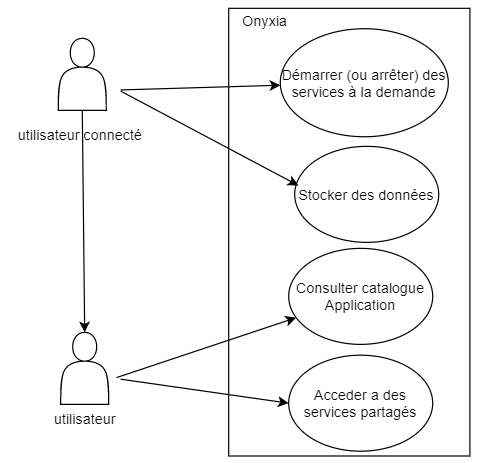
\includegraphics[scale=0.7]{Pictures/onyxia/onyxia-cu.PNG}
    \caption[]{Diagramme de cas d'utilisation \newline}
\end{wrapfigure}

La spécifité d'Onyxia est que l'ensemble des services à la demande qu'elle offre aux utilisateurs sont pré-configurés. Aucune configuration d'un point de vue technique n'est demandée à l'utilisateur. En effet, lors d'un déploiement, Onyxia agrège trois sources de données afin de configurer le service de l'utilisateur. \\

Onyxia-UI fournit des données provenant de deux sources : les données saisies par l'utilisateur (la mémoire ou le nombre de CPU alloué pour le service) et les données permettant l'accès aux autres services (la configuration git, vault et/ou minIO). Onyxia-API apporte, elle aussi, des informations comme le choix de l'URL du futur service déployé\footnote{Si deux utilisateurs possédaient chacun un service différent mais avec la même URL, les utilisateurs auraient tantôt accès à un service, tantôt à l'autre, de manière totalement aléatoire.}.\\

Ensuite, Onyxia-API dispose pour chaque service d'un squelette permettant de le déployer. Ce squelette est alors rempli à l'aide des valeurs précédemment créées.\\

Enfin, si le lancement du service n'est pas une simulation \footnote{En effet, onyxia permet à ces utilisateurs de lancer une application en mode simulation pour permettre aux personnes les plus motivées de découvrir la configuration de leurs services.}, Onyxia envoie le déploiement à l'orchestrateur, qui va désormais s'occuper de déployer et de maintenir en vie le service jusqu'à son extinction.

Ce workflow\footnote{Un workflow, ou « flux de travaux » ou encore « flux opérationnel » en français, est la représentation d'une suite de tâches ou opérations effectuées par une personne, un groupe de personnes, une application,... } est pour le moment uniquement réalisable avec Marathon et repose sur l'utilisation des Universes.\\




\begin{figure}[H]
\renewcommand{\figurename}{Diagramme}
\hspace{-1cm}
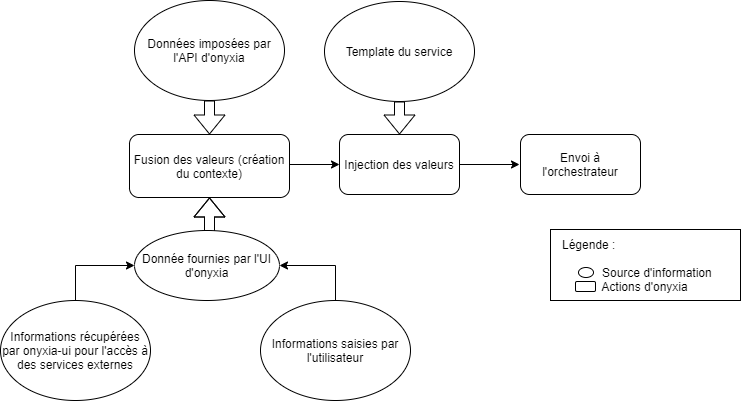
\includegraphics[scale=0.7]{Pictures/onyxia/onyxia-simplifie.png}
\captionsetup{margin=1.5cm,format=hang,justification=justified}
\caption[]{Processus de déploiement d'un service par Onyxia \newline}
\end{figure}



\section{Onyxia : Marathon et/ou Kubernetes ?}
Nous ne traiterons pas des solutions techniques mises en place (car elles n'ont pas grand intérêt), mais plutôt des points communs entre les deux solutions et des difficultés rencontrées, au cours de l'implémentation de Kubernetes dans Onyxia. Dans un premier temps, nous avions évoqué d'interfacer Onyxia avec Kubeapps un Chart Helm permettant de déployer des Charts Helm dans un cluster Kubernetes (voir en annexe \ref{kubeapps} pour plus de détails), mais la solution n'a finalement pas été retenue.\newline

Nous avons choisi l'outil Helm pour être l'équivalent de Universe dans le cadre de Kubernetes. Ce choix a été fait pour deux raisons : le nombre de charts Helm déja existant est conséquent, et les applications qui rendent un service équivalent (Kubeapps, Rancher,...) reposent sur cet outil. 
\subsection{Phase 1: Afficher des catalogues}
Au cours de cette première partie, nous allons comparer le format Universe et le format Helm dans le but d'en extraire des informations communes aux deux formats de templating. Si l'on compare la description du Universe.json \footnote{\url{https://Inseefrlab.github.io/Universe-Datascience/universe.json}} avec celle du index.yaml du répertoire Helm \footnote{\url{https://Inseefrlab.github.io/helm-charts-datascience/index.yaml}}, on remarque que les deux sont à peu de chose prêt composé d'une liste de paquets\footnote{L'universe n'est constitué que d'un tableau de paquets, alors que le index.yaml contient en plus la date de génération du fichier et la version de l'API Kubernetes avec laquelle ce Helm repository est compatible.}. \\ 

% \begin{wrapfigure}[21]{r}{0.4\textwidth}
% \renewcommand{\figurename}{Tableau}
% \begin{tabular}{@{}l l@{}}
% \toprule
% Universe package                              & Helm package                                  \\ \midrule
%     \begin{tabular}[c]{@{}l@{}}
% 	 \textcolor{green}{name} \\
%      \textcolor{green}{description} \\
% 	 \textcolor{green}{version} \\
%     \textcolor{blue}{marathon}\\
%     \textcolor{blue}{config}\\
%     packagingVersion \\
%     scm\\
%     maintener \\
%     website \\
%     framework
%     tags\\
%     preInstallNotes\\
%     postInstallNotes\\
%     postUninstallNotes\\
%     selected\\
%     lastUpdated\\
%     releaseVersion\\
%     resource\\
%     \end{tabular} & 
%     \begin{tabular}[]{@{}l@{}}
% 	 \textcolor{green}{name} \\
% 	 \textcolor{green}{description} \\
% 	 \textcolor{green}{version} \\
% 	 \textcolor{red}{urls} \\
% 	 apiVersion \\
% 	 appVersion \\
% 	 created \\
% 	 digest \\
% 	 engine \\
% 	 home \\
% 	 icon \\
% 	 keywords \\ 
% 	 sources \\
%     additionalProperties \\ \\   \\   \\
%     \end{tabular} \\ \bottomrule
% \end{tabular}
% \caption[]{}
% \end{wrapfigure}
\vspace{-1cm}
Dans la description des paquets, certains attributs sont communs comme le nom du paquet, la description ou encore la version.\newline

Il y a cependant une nette différence au niveau des fichiers de configurations et des templates. En effet, dans le cadre d'un paquet Universe, le template ainsi que la configuration (par défaut) sont directement dans la description du paquet alors que pour le paquet Helm (Chart), le fichier de templating ainsi que la configuration sont dans un fichier compressé disponible sur l'URL qui accompagne le paquet. \\



% \begin{figure}[H]\centering
% \renewcommand{\figurename}{Diagramme}
% 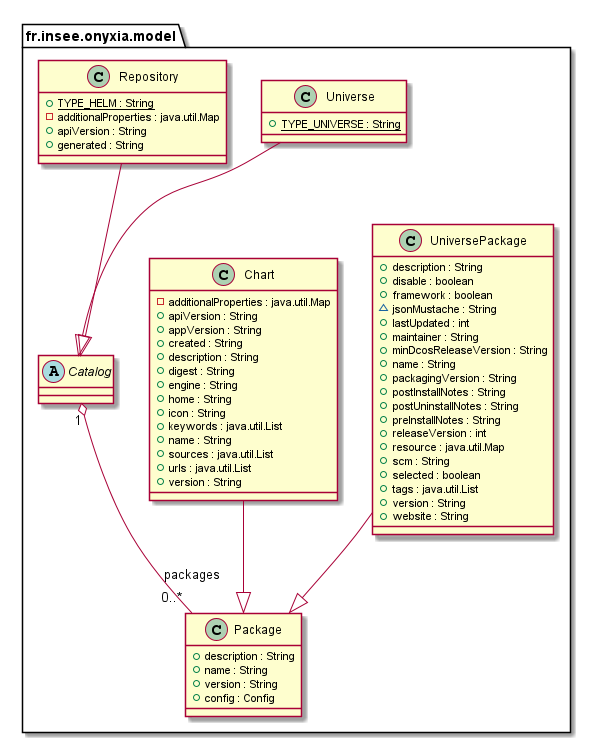
\includegraphics[scale=0.5]{Pictures/onyxia/testdiagram1.png}
% \captionsetup{margin=1.5cm,format=hang,justification=justified}
% \caption[]{Diagramme de classe des entitées catalogues et packages dans Onyxia \newline}
% \end{figure}
% \vspace{-2cm}
\begin{table}[H]
\hspace{-1.8cm}
\begin{tabular}{@{}lccl@{}}
\toprule
Attributs        & \multicolumn{1}{l}{Helm} & \multicolumn{1}{l}{Universe} & Description                                                                 \\ \midrule
name             & x                        & x                            & Nom du paquet                                                               \\
description      & x                        & x                            & Description du paquet                                                       \\
version          & x                        & x                            & Version du paquet                                                           \\
marathon         &                          & x                            & Objet contenant l'ensemble des templates du paquet (marathon.mustache.json) \\
config           &                          & x                            & Valeur par défaut servant à remplir le template (config.json)               \\
urls             & x                        &                              & Url du .tgz contenant les templates + values.json                            \\
postInstallNotes &                          & x                            & Note affichée après l'installation du paquets                               \\
icon             & x                        &                              & Icone du paquets                                                            \\
resource         &                          & x                            & Contient le nom de l'image docker utilisée et les icônes du paquets (resource.json)        \\ \bottomrule
\end{tabular}
\caption{Comparaison des principaux attributs décrivant un paquets Helm ou Universe \newline}
\label{tab:my-table}
\end{table}

\vspace{-0.5cm}
Pour avoir le même comportement (entre Helm et Universe), pour chaque Chart nous téléchargeons le fichier tgz du Chart (à partir de l'URL) et nous y récupérons le fichier de configuration. Ainsi, chaque paquet (Universe ou Helm) a au moins un nom, une description, une version et un fichier de configuration par défaut. Pour un paquet Universe nous stockons en plus le template de l'application. Cette étape n'est pas nécéssaire pour un Chart Helm, nous ajoutons juste le Chart a ceux connu par Helm (\textit{helm repo add...}).
\vspace{-0.5cm}
\begin{interrupt}
Un répertoire Helm ou Universe est vu comme un catalogue. Chacun de ces catalogues est composé de paquets qui peuvent être soit des Charts (Helm) ou des UniversePackages (Universe). Un paquet est au moins caractérisé par un nom, une description, une version et un fichier de configuration auquel s'ajoutent des informations appartenant à l'un ou l'autre des deux types de paquets. Le but de cette implémentation est d'être suffisamment standard pour pouvoir s'adapter à un potentiel futur nouveau orchestrateur.
\end{interrupt}

\begin{wrapfigure}[11]{l}{0.6\textwidth}
\renewcommand{\figurename}{Diagramme}
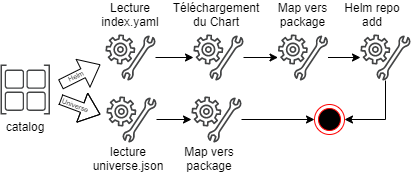
\includegraphics[scale=0.6]{Pictures/onyxia/workflow-catalog.png}
\caption{Workflow lecture et ajout de catalogues \newline}
\end{wrapfigure}
\vspace{-0.5cm}
L'ensemble des catalogues proposé par Onyxia est décrit dans un fichier json. Ce fichier comporte notamment le type du catalogue (Universe ou Helm) et l'URL sur lequel se trouve le fichier décrivant le catalogue (respectivement le universe.json ou le index.yaml). Le workflow ci-contre s'exécute alors périodiquement afin d'ajouter les différents paquets dans Onyxia.

\subsubsection{Difficultés rencontrées}
Au cours de cette première partie, la principale difficulté est venu des catalogues Helm. En effet, DC/OS propose une dépendance Maven permettant de convertir le fichier universe.json en objets Java. Il n'existe cependant pas d'équivalent pour Helm. Il a donc fallu implémenter à la main les classes pour réaliser la conversion de la description du répertoire Helm (index.yaml) en objet Java. Il a également fallu exécuter des commandes Helm (notamment pour l'ajout du répertoire dans Helm). Je n'ai trouvé aucune dépendance Java qui le permettait. Il a donc fallu ajouter à Onyxia un module permettant d'interagir avec Helm, par l'intermédiaire d'exécution de lignes de commande depuis java, ce qui a aussi impliqué d'ajouter Helm et Kubernetes à l'image docker d'Onyxia.

\subsection{Phase 2: Lancer des services et les configurer}
Cette partie débute au moment où l'utilisateur se retrouve sur la page de configuration de son service sur Onyxia. Que le service proviennent d'un paquet Universe ou Helm, l'expérience utilisateur est la même mais l'implémentation diffère. En effet, lors de la création d'un service on a le workflow \footnote{On ne fait pas apparaître ici comment Onyxia-ui récupère les informations techniques de l'utilisateur (Vault, Git, Minio)} suivant : 
\begin{figure}[H]\centering
\renewcommand{\figurename}{Diagramme}
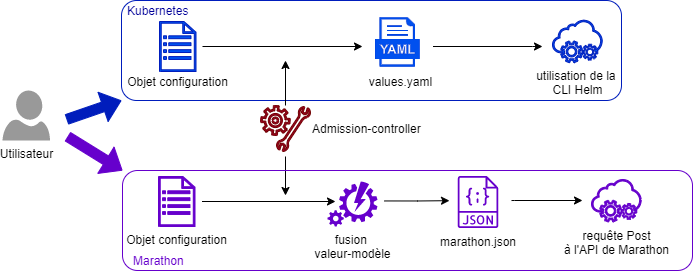
\includegraphics[scale=0.6]{Pictures/onyxia/publish-service.png}
\captionsetup{margin=1.5cm,format=hang,justification=justified}
\caption{Workflow du déploiement d'un service \newline}
\end{figure}

\vspace{-0.5cm}
Dans le cas Helm ou Universe, Onyxia-UI envoie la configuration du service à Onyxia-API. Onyxia-API reçoit les données de la configuration du service sous la forme d'une liste de clé-valeur. Cependant, il reste certains paramètres à injecter, par exemple : l'url, le nom du service, etc... c'est le rôle des admissions-controller.\\

Les admissions-controller parcourent l'ensemble de l'objet configuration, et y ajoute la clé et la valeur du paramètre qu'ils auront générés. Ainsi, dans le cas Universe et Helm, on ne possède pas les mêmes admissions-controller : \\
\begin{itemize}
    \item Pour Universe, on a un admission-controller qui va gérer le nom du service. En effet, Marathon ne possède pas la notion de namespace, mais plutôt de dossier \footnote{L'innovation a fait le choix que les services demandés par une personne se situent dans l'arborescence suivante users/idep/.} et ce dossier est déterminé en fonction de l'id du service. On doit donc injecter User-idep- dans le nom du service. Par ailleurs, un dossier ne peut pas contenir deux noms de service identiques, il faut donc randomiser le nom du service, l'admission controller ajoute un nombre aléatoire à la suite du nom du service (pour vs-code on aurait par exemple users/idep/vscode-1234).\\
    
    \item Universe utilise également un admission-controller qui va ajouter des labels (étiquettes) au service afin de le "marquer" comme un service déployé par Onyxia. \\
    
    \item Pour Universe et Helm, un autre admission-controller genère l'URL d'accès au service en fonction de l'idep du nom de service, du domaine sur lequel Onyxia est configuré pour déployer.\footnote{Pour éviter les doublons, ce générateur d'URLs ajoute un nombre aléatoire à l'URL.}. Cet admission-controller n'ajoute pas la même clé dans l'objet de configuration si il s'agit d'un service Universe ou Helm.\\
\end{itemize}
\vspace{-1cm}
\begin{interrupt}
\paragraph{Remarques:}
 Dans le cas de Helm, nous n'avons pas d'admission-controller qui injecte un id de service et/ou l'idep de la personne dans le nom du service, car ces derniers s'injectent au moment de l'exécution de la commande Helm par le biais des options. Helm permet l'injection du namespace (option -n) et la génération d'un identifiant randommisé (option --generate-name). \\
 
 Toujours dans le cas de Helm, la détermination du namespace de l'utilisateur entraîne sa création par Onyxia si ce dernier n'existe pas.
\end{interrupt}
Ensuite, dans le cas de Universe, le template du service est rempli (fichier mustache) à l'aide de l'objet contenant la configuration. Une fois cette opération réalisée, on a un fichier marathon.json classique rempli à l'aide des valeurs précédentes. Si il s'agissait d'un lancement de type simulation, alors on renvoie à l'utilisateur ce fichier, sinon on envoie ce fichier directement à Marathon par l'intermédiaire d'une requête POST.\\

Pour Helm, on traduit l'objet contenant la configuration en un fichier de type values.yaml et on exécute la ligne de commande \texttt{Helm apply my-app -f my-values -n namespace} avec ou sans l'option \texttt{--dry-run} en fonction de la demande de l'utilisateur (simulation ou non). C'est donc Helm qui se charge de la récupération du template, de l'injection des valeurs ainsi que de la communication à Kubernetes du déploiement.

\subsubsection{Difficultés rencontrées}
Durant cette partie, les difficultés sont venues de la partie Helm. En effet, DC/OS propose un client Marathon (pour dialoguer directement avec Marathon), et il existe une dépendance maven facilitant le remplissage des templates \footnote{Lien vers le projet: \url{https://github.com/spullara/mustache.java}}.\newline

Pour pouvoir installer une application en utilisant Helm, il fallait d'abord que l'utilisateur possède un namespace dans Kubernetes. Pour cela, nous avons dû autoriser Onyxia à créer des namespaces et faire en sorte qu'Onyxia puisse dialoguer avec Kubernetes. Il existe deux bibliothèques pour communiquer avec Kubernetes depuis Java, l'officielle (\url{https://github.com/kubernetes-client/java}) et celle proposé par fabri8 (\url{https://github.com/fabric8io/kubernetes-client}. Ces deux bibliothèques communiquent avec l'API de Kubernetes (et non avec kubectl). Nous avons choisi la deuxième car elle est plus complète et plus simple d'utilisation. \newline

Afin qu'Onyxia puisse créer des namespaces, il fallait lui donner des droits dans le cluster Kubernetes. Initialement, nous voulions lui donner les droits cluster-admin\footnote{L'application a le droit de créer toute sorte de ressources dans le cluster.} uniquement sur l'ensemble des namespaces commençant par "user-..." (c'est-à-dire les namespaces qu'Onyxia devait gérer et servant à déployer les services des utilisateurs). Mais cela n'est pas possible actuellement\footnote{issue disponible ici : \url{https://github.com/kubernetes/kubernetes/issues/56582} fermée mais non résolue}, nous lui avons donc donné le rôle cluster-admin (ce n'est pas idéal puisque Onyxia pourrait donc interférer sur des namespaces qui ne lui sont pas dédiés).

\subsection{Phase 3: Récupérer des services, leurs configurations et les arrêter}
La partie consistant à récupérer les services, leurs configurations et à pouvoir les stopper a sûrement été la plus facile dans la mise en place. Des différences subsistent néanmoins dans le comportement des 2 orchestrateurs. \\

La principale différence réside dans le fait que pour les paquets Universes, l'ensemble des actions se fait par l'intermédiaire du client Marathon  et les résultats sont lu à l'aide des classes fournies par DC/OS. Alors que dans le cas des paquets Helm, l'ensemble des actions se fait depuis Helm ce dernier et encore une fois aucune librairie facilitant la lecture des résultats n'existe.\\

\begin{table}[H]
\hspace{-1.5cm}
\begin{tabular}{@{}lll@{}}
\toprule
                                                                                     & Universe             & Helm                                                                                                                             \\ \midrule
Arrêter un service                                                                   & requête sur endpoint & Helm rm nomRelease -n namespace                                                                                                  \\
\begin{tabular}[c]{@{}l@{}}Lister mes services + \\ Détail d'un service\end{tabular} & requête sur endpoint & \begin{tabular}[c]{@{}l@{}}Helm ls -n namespace + \\ Helm get manifest nomRelease -n namespace pour chaque release\end{tabular} \\ \bottomrule
\end{tabular}
\end{table}
Pour Marathon, lister les services d'un utilisateur nécéssite de réaliser une requête à l'orchestrateur en précisant le dossier de l'utilisateur. L'utilisateur pouvant déployer des services dans ce dossier par d'autre moyen qu'Onyxia, nous rajoutons un filtre sur les labels : seul les déploiement ayant un label Onyxia doivent-être renvoyé.\\

Pour Helm, chaque requête sur Onyxia-API pour lister mes services résulte en fait en n+1 requêtes. En effet, coté API on doit d'abord exécuter une première ligne de commande pour lister le nom des services qui s'exécutent dans le namespace de l'utilisateur (et ou uniquement Onyxia à le droit de déployer). Ensuite, il faut faire une requête par service pour récupérer les détails le concernant. Ce qui conduit au final à n+1 requêtes (en comparaison, il suffit d'une seule requête pour les paquets Universes). \\

Par ailleurs, le comportement de Kubernetes n'est pas le même que Marathon lorsqu'on stoppe un service. En effet, Marathon distingue un service arrêté d'un service supprimé, ce n'est pas le cas de Kubernetes. Un service Helm que l'on arrêtera sera perdu (il faudra repasser par l'étape de création pour en avoir un nouveau) alors qu'un service Universe déployé dans Marathon pourra être redémarré.

\section{Quels besoins de sécurité ?}
Dans le cadre d'une architecture conteneurisée il faut également mettre en place des mécanismes de sécurité. Dans le cadre de la plateforme innovation, deux critères sont importants à vérifier : la disponibilité et le traçage. La confidentialité et l'intégrité n'est pour le moment pas du tout garantie. En effet cette plateforme reste tout de même une plateforme de "tests".\\

La disponibilité de la plateforme de l’innovation est un sujet très important. En effet, chaque jours plusieurs dizaine de services à la demande et d’environnements de tests sont crées. Si l’orchestrateur qui gère l’ensemble de ces tâches venait à tomber, c’est plusieurs centaines de personnes qui seraient donc pénalisées. La disponibilité des services est donc primordiale. Pour garantir une disponibilité optimale, il faut tout d’abord pouvoir identifier les risques pouvant la réduire : perte de node, redémarrage d’un conteneur, manques de ressources, etc... \\

Afin de se prémunir de certains problèmes il est important de disposer d’outils de surveillance au sein du cluster. En plus des outils natifs proposé par DC/OS ou par Kubernetes (les différents dashboards), on retrouve des outils externes disponibles sur les 2 orchestrateurs.\\

Les 2 orchestrateurs permettent de déployer facilement l'outil Prometheus et Grafana. Cet outil va permettre d'agréger l'ensemble des métriques disponibles dans le cluster au même endroits. 

Ce même outil permet de réaliser de la traçabilité. Il est important de pouvoir suivre le parcours d'un utilisateur. Hormis les outils de monitoring tel que les dashboards ou Prometheus Grafana, il existe des outils, (dont le déploiement est nettement facilité pour Kubernetes) qui permettent de suivre le parcours des requêtes émisent par l’utilisateur.\\

La CNCF\footnote{Cloud Native Computing Foundation} recommande l’utilisation de l’outil Jaeger afin de réaliser du traçage au sein d’une architecture conteneurisée. Le traçage permet de visualiser les requêtes et de construire une vue de l’ensemble de la chaîne des appels effectués, des demandes des utilisateurs aux interactions entre des centaines de services. Il permet également d’évaluer la latence des applications (le temps de réponse à chaque demande), de suivre le cycle de vie des appels sur le réseau (HTTP, RPC, etc.) et d’identifier les problèmes de performances en obtenant une visibilité sur les goulets d’étranglement.\\

L'annexe \ref{securite} propose des informations complémentaires sur les sources de failles de sécurité dans un cluster, un zoom sur le fonctionnement de Prometheus-Grafana, et quelques proposition de pratiques plus ou moins simple à mettre en place afin de garantir une sécurité optimale. 








\part{\textcolor{ocre}{Conclusion et annexes}}
\chapterimage{/chapter-image/conclusion.png}
\chapter{Conclusion}
\vspace{-2cm}

Après l'analyse des besoins d'intégration et de déploiement en continu pour les développeurs, et de service à la demande pour les statisticiens, la nécessite de posséder une architecture dite conteneurisée à l'Insee semble évidente. \newline

De nombreuses solutions existent sur le marché, mais 2 auront retenue notre attention, Kubernetes et Mesos/Marathon. Le premier car c'est actuellement le leader mondial dans ce domaine, le deuxième puisque c'est la solution actuellement en place à l'Insee. \newline

Ce stage a été l'occasion de comparer leur architecture et de s'approprier leur fonctionnement. Kubernetes semble s'imposer comme la solution à retenir pour la mise en place d'une potentielle future architecture conteneurisée en production.\newline

Ce stage a également mis en avant, pour les développeurs, l'importance  de savoir créer et utiliser des images Docker, puisqu'ils sont à la base d'une architecture conteneurisée.\\

Enfin, mes recherches dans le cadre de l'intégration continue, m'ont conduit a découvrir des outils (Argo), encore jamais utilisé à l'Insee, et qui facilite l'exploitation des conteneurs. Ces recherches ont sensibilisé, je pense, le public sur l'importance des travaux qu'il reste encore à réalisé à l'Insee afin d'améliorer les processus d'intégration continue.\\

L'ensemble des travaux réalisés sur Onyxia présente de multiples intérêts : indépendance de DC/OS, ajout de fonctionnalités augmentant la disponibilité de l'application, et surtout l'application est désormais open-source. L'ajout du support de Kubernetes lui procure également une meilleure visibilité.\\


En effet, l'Insee peut désormais proposer aux autres établissements du ministère des Finances une solution pour se créer un cloud spécialisé dans les outils et techniques de traitement de données. De plus, cette solution est à l’état de l’art, accessible à un public varié, 100\% gratuite et opensource.\\

Elle a d'ailleurs été utilisé par la communauté spyrale (une communauté d'agents de l'Etat) qui durant la période de confinement, a proposé aux agents intéressés de les accompagner dans un parcours de formation. Cette plateforme permet donc de rendre les techniques modernes plus accessibles et de mutualiser les efforts pour répondre aux défis actuels de la statistique publique.\\



% Plus personnellement, ce stage m'aura permis de découvrir plus en profondeur le cloud et ses usages, et de monter en compétence sur des domaines très prisés actuellement. Ce stage m'a également appris a m'adapter rapidement, en effet le confinement m'ayant privé des ressources interne de l'Insee (dans un soucis d'économie des ressources le cluster REST interne a été débranché), il a fallu que je m'adapte rapidement.
\appendix


\chapterimage{chapter-image/architecture-01.jpg} 
\chapter{Architecture et fonctionnement}
\vspace{-2cm}
\label{Architecture}

\section*{Architecture d'un cluster Kubernetes}
Un cluster Kubernetes (k8s) a obligatoirement au moins un worker node. Le worker node est le serveur qui bénéficie de la plus grosse configuration en termes de CPU, mémoire, RAM puisque c'est lui qui fait tourner les conteneurs (et donc les applications).\newline 

Dans un cluster k8s, le  master node est appelé control plane. Il gouverne les worker-nodes (et donc les Pods\footnote{Un Pod est un groupe d'un ou plusieurs conteneurs (comme des conteneurs Docker), ayant du stockage/réseau partagé, et une spécification sur la manière d'exécuter ses conteneurs.}) du cluster. Dans les environnements de production, afin de garantir une disponibilité de service optimale ,le control plane est répliqué sur plusieurs machines et le cluster est composé de plusieurs worker nodes, qui sont, dans le cas idéal, répartis géographiquement pour garantir une qualité de services optimale (réduction de la latence).\newline

Nous ne parlerons pas ici des public nodes. En effet, dans le cadre du stage nous avons utilisé un cluster k8s fourni par GCP (google), et dans ce cas l'ensemble de la configuration des publics nodes est gérée par le fournisseur cloud.


\subsection*{Les composants du control-plane}
Les composants du control plane (qui correspond au Master-node) sont ceux qui gèrent l'état global du cluster, qui détectent et réagissent en fonction des événements au sein du cluster (déploiement d'une nouvelle application ,load-balancing\footnote{répartition des requêtes sur les diverses instances d'une même application}, etc...). De manière générale, même si les composants du control plane peuvent être installés sur différentes machines, les scripts classiques déploient l'ensemble des composants du control-plane sur une seule et unique machine, sur laquelle aucun conteneur créé par un utilisateur ne peut être lancé.

\paragraph*{Etcd}
Le Master node possède une base de données clés valeurs \footnote{Base de données non relationnelle qui utilise une méthode clé-valeur simple pour stocker des données. Une base de données clé-valeur stocke les données sous forme de paires clé-valeur dans lesquelles une clé sert d'identifiant unique}, où est stocké l'état du cluster Kubernetes. Elle est appelée etcd.

\paragraph*{Kube-apiserver}
L'api-server est le composant du Kubernetes control-plane qui expose l'API de Kubernetes. L'api-server est donc le point d'entrée pour l'ensemble des opérations à exécuter sur le cluster, elle fait office de passerelle vers le cluster. Elle reçoit des requêtes HTTP, elle les valide et met à jour les objets correspondants dans l'Etcd. Par définition, l'api-server doit être accessible par des clients extérieurs au cluster. Alors que les worker nodes, et donc les conteneurs, peuvent ne pas l'être. En effet, dans le cas de débuggage, l'api-server peut aussi être utilisée comme un point d'entrée vers les nodes et les Pods.


\paragraph*{Kube-controller manager}
Le kube-controler manager est le composant qui contrôle l'état du cluster en continue. Dans le monde de Kubernetes, un contrôleur est un processus qui tourne en boucle : il interroge l'api-server qui lui renvoie l'état du cluster et il effectue les changements (toujours en passant par l'api-server) de manière à ce que le cluster tende toujours vers l'état désiré. Kubernetes possède 4 contrôleurs (initialement, mais on peut en rajouter pour d'autres besoins\footnote{Afin d'exposer nos services, on a besoin d'ingress. L'ingress-controller permet par exemple de scanner l'ensemble des objets ingress et de les ajouter à sa pile.}), regroupés en un seul contrôleur: le controller-manager. Ce dernier regroupe les 4 contrôleurs suivants: 
\begin{itemize}
    \item Node Controller : c'est le contrôleur qui détecte les nodes en pannes et qui agit en conséquence.
    \item Replication Controller : Il vérifie si le cluster contient bien le bon nombre de Pods pour chaque objet ReplicationController (attention on parle ici de l'objet replicationController\footnote{Un replicationController est un objet qui décrit, pour un déploiement donné, combien de réplicas d'une application sont nécessaires} et non du contrôleur en lui même).
    \item Endpoints Controller: Il définit les objets Endpoints (c’est-à-dire les Services qui sont reliés aux Pods).
    \item Service Account et Token Controllers : C'est la partie responsable de la création des comptes par défaut et des jetons d'accès à l'API pour les nouveaux namespaces\footnote{Kubernetes prend en charge plusieurs clusters virtuels présents sur le même cluster physique. Ces clusters virtuels sont appelés namespaces.}.
\end{itemize}

\paragraph{Le cloud-controller manager}
Ce composant permet de lier le cluster Kubernetes à la logique du fournisseur cloud. C'est une surcouche qui n'est pas toujours présente (notamment dans le cas d'une installation dite on-premise\footnote{Une installation on-Premise est une installation réalisée de A à Z sans passer par un fournisseur. L'entreprise installe toute les briques nécessaires une par une et en assure la gestion par ses propres moyens.}). Il permet notamment au fournisseur cloud d'ajouter des routes dans le cluster (à la manière d'un reverse proxy). Il ajoute également un volume-controller afin de pouvoir créer des Volumes \footnote{Un volume est un espace de stockage, indépendant du conteneur, ce qui permet de persister des données et de les récupérer même si le conteneur vient a être tuer.} et interagir avec le fournisseur cloud pour les orchestrer.

\paragraph*{Le kube-scheduler}
Le kube-scheduler est le composant du master node qui est responsable de la surveillance des Pods qui viennent d'être créés. En effet, Kubernetes autorise les utilisateurs à lancer sur le cluster des conteneurs. Le kube-scheduler choisi automatiquement quel(s) node(s) va accueillir le ou les conteneurs nouvellement créé(s). Le scheduler détecte les Pods qui ne sont pas affectés, et il les associe à des nodes par le biais de l'api-server, en fonction des besoins et des ressources disponibles.

\subsection*{Les composants du Node}
Chaque composant que nous allons voir ici, est exécuté sur chaque node. Ils maintiennent les Pods en vie et fournissent l'environnement d'exécution Kubernetes. Les nodes sont parfois aussi appelés worker-nodes.

\paragraph*{Le Kubelet}
Le kubelet est le principal composant qui s'exécute sur chaque node. Il peut enregistrer le node auprès de l'api-server en utilisant l'un des éléments suivants : le nom d'hôte, un flag\footnote{Une annotation servant d'identifiant} pour remplacer le nom d'hôte ou une logique spécifique pour un fournisseur de services cloud.\\

Le kubelet fonctionne en termes de PodSpec. Un PodSpec est un objet (un contrat) Kubernetes qui décrit un Pod. Le kubelet prend un ensemble de PodSpecs qui sont fournis par divers mécanismes (principalement par l'api-server) et s'assure que les conteneurs décrits dans ces PodSpecs fonctionnent et sont en bonne santé.

\paragraph*{Le Kube-Proxy}
Kube-proxy est un proxy réseau qui s’exécute sur chaque node du cluster et implémente une partie du mécanisme de Service Discovery.

\paragraph*{Le Container-Runtime}
Le Container-Runtime est le logiciel responsable de l’exécution des conteneurs.\\


En résumé, on peut schématiser un cluster Kubernetes de la manière suivante :

\begin{figure}[H]\centering
\renewcommand{\figurename}{Schéma}
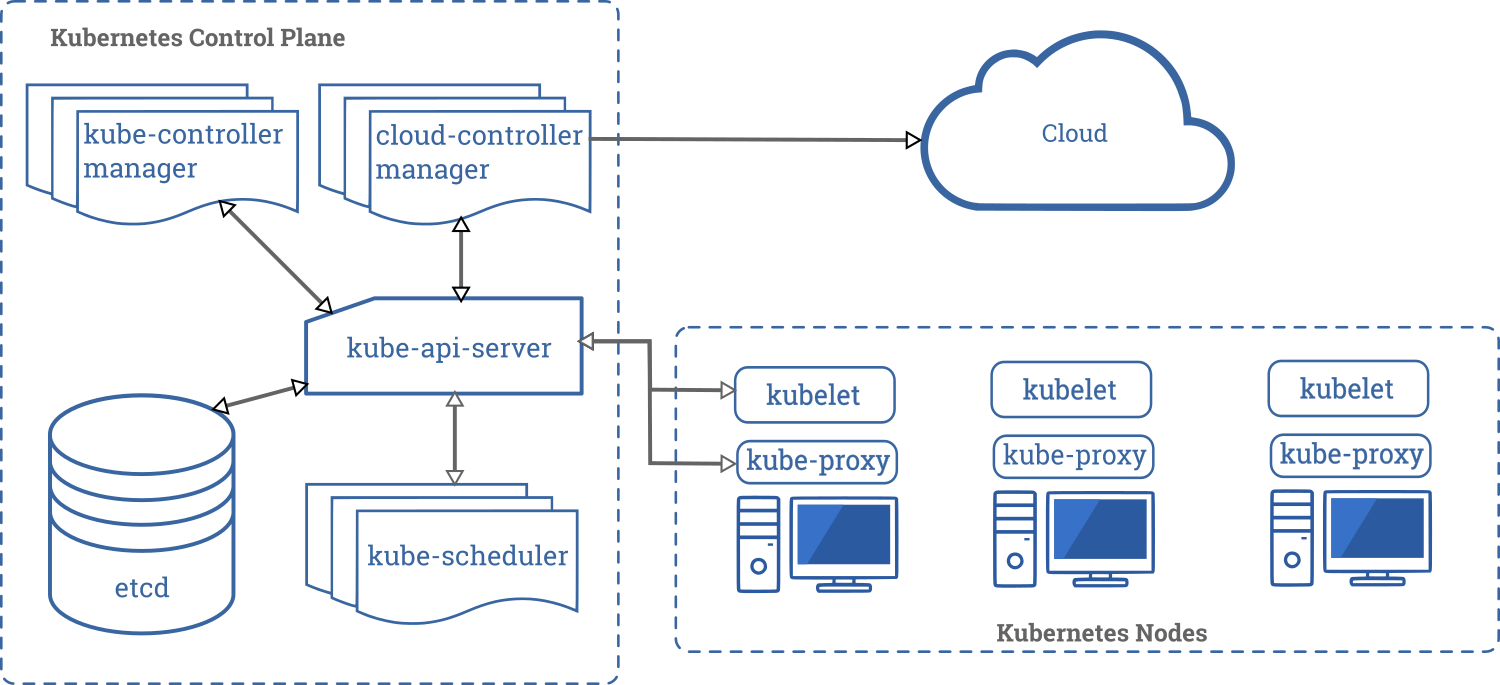
\includegraphics[scale=0.1]{Pictures/Comparaison/Kubernetes-cluster-archi.png}
\captionsetup{margin=1.5cm,format=hang,justification=justified}
\caption[]{Architecture d'un cluster Kubernetes \newline}
\end{figure}



\begin{interrupt}
\paragraph{Conclusion:}
Un cluster Kubernetes fonctionne de la manière suivante :
sur chaque noeud, on retrouve le kubelet et le kube-proxy qui sont chargé du déploiement, de la surveillance, et de la mise en réseau des conteneurs. Le kubelet communique avec l'api-server afin de communiquer l'état de ses conteneurs que l'API va stocker dans l'Etcd.\newline

L'api Server reçoit les requêtes, elle vérifie les commandes envoyées à l'aide du controller manager, elle enregistre les actions dans l'etcd et le kube-scheduler va répartir les déploiements sur les différents nodes.
\end{interrupt}

\section*{Architecture d'un cluster Mesos/Marathon}
Tout d'abord, il faut savoir qu'il est impossible d'utiliser l'orchestrateur de conteneur Marathon, sans posséder au préalable un cluster Mesos. Nous allons ici expliquer comment un cluster Mesos fonctionne et comment Marathon s'articule autour de cette architecture.



% control plane c'est du mesos ou kubernetes ??
% - v2 : L'équivalent du control plane est le master node pour un cluster Mesos.
\subsection*{Les composants du control plane}
Dans le cadre d'un cluster Mesos le master node est aussi appelé control-plane. Il abrite deux entitées, le Mesos master et les Mesos frameworks.
\paragraph*{Le Mesos master}
Le Mesos master est le cœur du cluster. Il garantit la haute disponibilité du cluster. Il héberge l'interface utilisateur qui fournit des informations sur les ressources disponibles dans le cluster. L'API Mesos est accessible par ligne de commande ou directement par requête HTTP. Le Mesos master est la source centrale de toutes les tâches en cours, il est la source de vérité dans le cluster. Il stocke en mémoire toutes les données relatives aux tâches, à l'état du cluster. Pour une tâche, il ne stocke que les informations nécessaires, ce qui permet au master de fournir à l'interface utilisateur les données relatives aux tâches avec une latence minimale. C'est le master qui alloue les ressources aux différents frameworks Mesos.

\paragraph*{Les schedulers}
Le scheduler est en fait un des deux composants des Framework Mesos. Le framework Mesos est composé de deux éléments : le scheduler et l'executor. Le premier étant situé dans le control plane et le deuxième dans les Mesos agents (équivalent des worker-nodes) rattachés à ce framework\footnote{Mesos permet d'assigner, ou non, des worker-nodes à un seul framework uniquement}. On s'intéresse ici uniquement au scheduler. \\

Lorsqu'il est déployé, le scheduler s'enregistre auprès du master Mesos et obtient un identifiant. A chaque requête reçue par le Mesos master, ce dernier délègue la requête au bon scheduler. Lorsque le scheduleur reçoit la requête, il évalue si il peut satisfaire la demande (par exemple déployer une application) en fonction des ressources que le Mesos master met à sa disposition. Il est également responsable de la gestion des échecs et des erreurs des tâches qu'il doit gérer. \\
\paragraph*{Marathon}
Marathon est un des scheduler qui peut être déployé dans Mesos. Marathon est même un des piliers de l'architecture des clusters Apache Mesos. Utilisé en production pour l'orchestration de conteneurs, Marathon fournit une API REST pour le démarrage, l'arrêt et la mise à l'échelle des applications. Écrit en Scala, Marathon peut fonctionner en mode haute disponibilité en exécutant plusieurs copies de lui même. L'état des tâches en cours d'exécution est stocké dans la base de données du Mesos master.\\

Marathon est en fait un méta-scheduler, ce qui signifie qu'il peut démarrer d'autres schedulers Mesos tels que Chronos ou Storm. Marathon en tant qu'orchestrateur de conteneur va s'assurer qu'ils survivent aux pannes de machine. Il peut lancer tout ce qui peut être lancé dans un shell standard. (On peut même lancer une autre instance de Marathon via Marathon.)

\subsection*{Les composants du Mesos agent}
Un cluster Mesos est composé de plusieurs Mesos agent, ce sont les équivalent des workers nodes. L'ensemble des tâches va donc s'éxécuter sur ces machines. Sur chaque Mesos agent on retrouve trois composants : le ou les schedulers locaux ainsi que leur executor associé et un processus appelé Mesos agent. Le Mesos agent fournit au Mesos master les informations relatives à l'hôte dans lequel il s'exécute (y compris les données sur les tâches en cours, les ressources disponibles de l'hôte qui lui sont allouées et d'autres métadonnées).

\paragraph*{Le scheduler local}
Le scheduler local communique avec le Mesos agent pour lui fournir l'état des tâches dont il a la responsabilité (l'état des applications pour Marathon par exemple). Si l'état des tâches ne correspond pas à celui attendu, il va communiquer les informations nécessaires à l'executor pour tendre vers le bon état.

\paragraph*{L'executor}
L'executor exécute la tâche demandée par le scheduler (relayée par le scheduler local) et notifie en retour le statut de chaque tâche.


\begin{figure}[H]\centering
\renewcommand{\figurename}{Schéma}
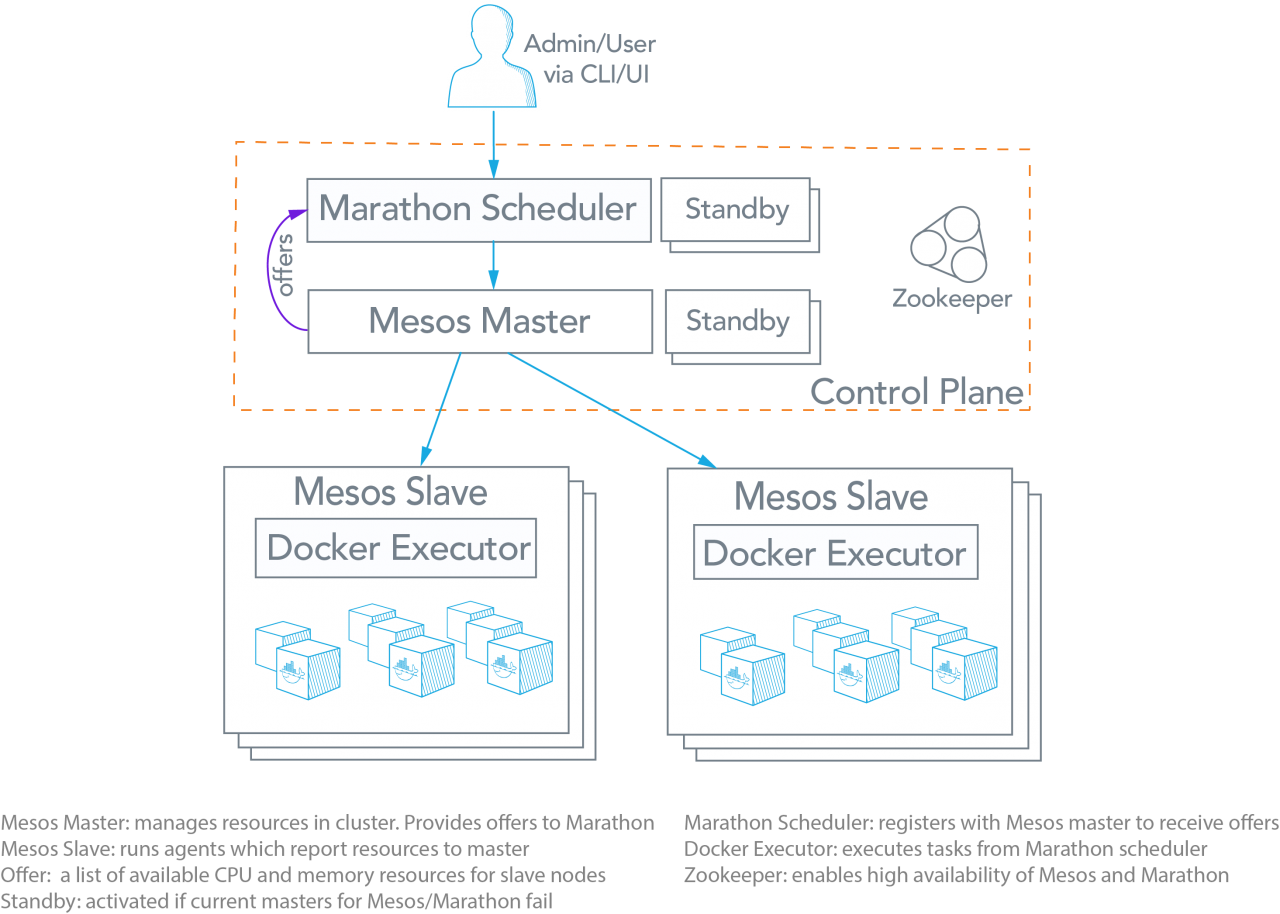
\includegraphics[scale=0.35,trim={0 5cm 0 0},clip]{Pictures/Comparaison/mesos-architecture.png}
\captionsetup{margin=1.5cm,format=hang,justification=justified}
\caption[]{Architecture simplifié d'un cluster Mesos \newline}
\end{figure}



\chapterimage{/chapter-image/deployer.png}
\chapter{Déployer une Application}
\label{A}
\vspace{-2cm}
\section*{Marathon: le endpoint /v2/deployments}
Il faut savoir que un déploiement dans Marathon ce fait par l'intermédiaire d'un fichier JSON décrivant l'état souhaité du déploiement. Nous allons partir de l'exemple ci dessus qui permet de déployer dans Marathon un vs-code permettant de faire du python.
\usemintedstyle{friendly}
\begin{minted}[mathescape,
               linenos,
               numbersep=5pt,
               gobble=2,
               frame=lines,
               framesep=2mm]{Json}

  {
    "id": "/users/ystfg5/vscode-8073154573408695635",
    "instances": 1,
    "cpus": 0.1,
    "mem": 2048,
    "container": {
      "type": "DOCKER",
      "docker": {
        "image": "inseefrlab/vscode-python",
        "network": "BRIDGE",
        "forcePullImage": false,
        "portMappings": [
          {
            "containerPort": 8080,
            "hostPort": 0,
            "labels": {}
          }
        ],
        "privileged": false
      }
    },
    "env": {
      "PASSWORD": "Changeme",
    },
    "labels": {
      "HAPROXY_0_VHOST": "amodifier.portail.innovation.insee.eu",
      "HAPROXY_0_REDIRECT_TO_HTTPS": "true",
      "HAPROXY_0_ENABLED": "true",
    },
    "fetch": [
      {
        "uri": "https://git.lab.sspcloud.fr/innovation/plateforme-onyxia/
                services-ressources/-/raw/master/onyxia-init.sh",
        "executable": true,
        "extract": false,
        "cache": false,
        "destPath": "onyxia-init.sh"
      }
    ],
  }

\end{minted}
Si on découpe le contrat ci dessus on a les parties suivantes : 
\begin{itemize}
    \item id : l'id corresponds au dossier (virtuel) auquel va être rattaché le conteneur. Cela permet d'isoler les ressources entre utilisateur.
    \item container : Ici on déclare l'image que l'on va vouloir déployer
    \item env : Cette balise permet d'ajouter des variables d'environnement directement disponible au sein du conteneur. Ici on injecte la conf git de l'utilisateur   
    \item labels : Dans Marathon, la configuration du reverse proxy se fait par l'intermédiaire des labels. Il a été choisit d'utiliser HA\_PROXY comme reverse-proxy. Ce dernier scanne l'ensemble des déploiements dans Marathon en continue. Lorsqu'il trouve l'annotation HAPROXY\_0\_VHOST il sait qu'il va devoir exposer ce déploiement, il ajoute alors ce conteneur à sa table de déploiement ce qui lui permettra de faire le lien entre l'url demandé et le service correspondant lorsqu'une requête demandant l'accès a ce service arrivera.   
    \item instance: le nombre de réplique l'on veut du service.
    \item fetch: cette partie indique a Marathon d'aller télécharger le fichier correspondant et de l'ajouter à la mesos-sandbox (un espace de stockage accessible à ce conteneur).
\end{itemize}
\section*{Kubernetes : le trio ingress.yaml, service.yaml, deploiement.yaml}

Tout d'abord,il faut savoir que les déploiements Kubernetes sont, en général, configurés dans des fichiers .yaml (équivalent de JSON). Pour ce Hello world, nous allons également tenter de déployer un vscode. Nous allons avoir besoin de 3 fichiers (on peut néanmoins les regrouper en 1 seul fichier mais pour plus de lisibilité nous les séparerons) 

\subsection*{Deployment.yaml}
Un deployment correspond à l'orchestration de Pods. Le deployment s'assure que l'application tourne bien, avec un nombre d'instances correspondant au nombre demandé. Si l'on regarde le fichier deployment.yaml : 
\usemintedstyle{friendly}
\begin{minted}[mathescape,
               linenos,
               numbersep=5pt,
               gobble=2,
               frame=lines,
               framesep=2mm]{yaml}
    apiVersion: apps/v1
    kind: Deployment
    metadata:
      name: vs-code
      namespace: test
    spec:
      replicas: 1
      selector:
        matchLabels:
          app: vs-code
      template:
        metadata:
          labels:
            app: vs-code
        spec:
          volumes:
          - name: vs-code-data
            emptyDir: {}
          containers:
          - name: vs-code
            image: inseefrlab/vscode-python:latest
            env:
            - name: PASSWORD
              value: changeme
            volumeMounts:
            - mountPath: "/data"
              name: vs-code-data
          initContainers:
          - name: toto
            image: ubuntu:xenial
            command:
            - "/bin/sh"
            - "-c"
            args:
            - apt update
            - apt install -y wget
            - cd /data
            - wget https://git.lab.sspcloud.fr/innovation/plateforme-onyxia
                    /services-ressources/-/raw/master/onyxia-init.sh
            volumeMounts:
            - mountPath: "/data"
              name: vs-code-data
\end{minted}

On retrouve les informations intéressantes suivantes: 
\begin{itemize}
    \item le champ replicas qui corresponds au nombre de conteneurs que l'on va lancer dans le cluster. On parle alors de scalabilité horizontale. 
    \item le champ image qui corresponds à l'image docker que nous allons déployer dans Kubernetes.
    \item le champs env qui va nous permettre de passer des variables d'environnement au conteneur.
    \item le champs volume permet de déclarer un volume et le type de ce dernier. Ce volume sera ensuite attaché au conteneur avec l'entrée volumemounts.
    \item le champs init container. Un init container est un conteneur qui s'executent avant notre déploiement afin de réaliser une certaine tache. Ici on va récuperer le fichier avec un wget et on le place dans un repertoire qui sera commun avec le conteneur que l'on veut déployer. Un init container pourrait très bien servir à requêter une API, ou à faire des tests sur l'existence d'un autre conteneur avant de démarrer.
    \item les autres champs sont essentiellement des champs qui serviront a Kubernetes comme identifiant.\\
\end{itemize}

Envoyons à Kubernetes le fichier que l'on vient de créer, pour cela nous utiliserons la ligne de commande kubectl:
\usemintedstyle{friendly}
\begin{minted}[mathescape,
               linenos,
               numbersep=5pt,
               gobble=2,
               frame=lines,
               framesep=2mm]{shell}
               kubectl apply -f nomDuFichier.yaml
\end{minted}
Kubectl est la ligne de commande qui nous permet de communiquer avec le cluster Kubernetes. Cette cli transforme l'ensemble des commandes en requêtes http qu'elle envoie sur les bons endpoints\newline

Notre Pod est désormais deployé, mais il tourne dans le cluster mais impossible d'accéder à ce déploiement. 
\subsection*{Service.yaml}
Chaque Pod possède une adresse IP qui lui est propre, on pourrait donc imaginer donné accès a cette adresse ip aux utilisateurs. Mais lorsqu'on diffuse une application, on expose un service qui sera rendu par un ou plusieurs Pod, donner l'ip du Pod aux utilisateurs n'est donc pas le meilleur moyen. De plus, tous les clients de l'application (en particulier les autres microservices du cluster) n'ont pas à savoir où sont les Pods précisemment. \\

Par ailleurs, Kubernetes propose et impose un découplage fort entre le service rendu et l'application qui le rend. \\ 

Le concept de service va donc nous aider. Un service permet d'exposer un port du conteneur (ici, le port 8080 de notre vscode) à l'intérieur du cluster (on ne parle pas encore d'exposition vers l'extérieur, ça viendra avec le concept suivant). \\
Le contrat du service est le suivant : 
\usemintedstyle{friendly}
\begin{minted}[mathescape,
               linenos,
               numbersep=5pt,
               gobble=2,
               frame=lines,
               framesep=2mm]{yaml}
    apiVersion: v1
    kind: Service
    metadata:
      name: vs-code
    spec:
      ports:
      - name: http
        port: 80
        targetPort: 8080
      selector:
        app: vs-code
\end{minted}
Les infos les plus importantes sont : 
\begin{itemize}
    \item name : le nom donné au port exposé (sera utilisé plus tard)
    \item targetPort : le port du conteneur (pour vscode : 8080)
    \item port : le port sur le service (non utilisé dans ce tutoriel) mais il permet a un autre conteneur de venir interrogé ce service.\\
\end{itemize}

Après exécution du service.yaml (avec kubectl apply) le service est bien en place, notre vscode est maintenant accessible mais ... uniquement depuis l'intérieur du cluster. (pour s'en convaincre \textit{kubectl get services} noter l'adresse ip, puis lancer  \textit{kubectl run -i --tty busybox --image=busybox --restart=Never -- sh } qui permet de lancer un déploiement en mode interactif et nous donne accès a son shell, exécuter ensuite curl adresse-ip:8080 notre service répond)

\subsection*{Ingress.yaml}
L'ingress est le fichier qui va nous permettre d'exposer notre service a l'extérieur du cluster. Un ingress correspond à un point d'entrée dans le cluster. Ca va nous permettre d'exposer notre service en dehors du cluster ! C'est globalement équivalent au travail classique d'un reverse-proxy.

\usemintedstyle{friendly}
\begin{minted}[mathescape,
               linenos,
               numbersep=5pt,
               gobble=2,
               frame=lines,
               framesep=2mm]{yaml}
    apiVersion: networking.k8s.io/v1beta1
    kind: Ingress
    metadata:
      name: vs-code
      annotations:
        kubernetes.io/ingress.class: nginx
    spec:
      tls:
      - hosts:
        - amodifier.portail.innovation.insee.eu
      rules:
      - host: amodifier.portail.innovation.insee.eu
        http:
          paths:
          - path: "/"
            backend:
              serviceName: vs-code
              servicePort: 80
\end{minted}
Quelques informations importantes :

\begin{itemize}
    \item \texttt{annotations: Kubernetes.io/ingress.class: nginx} : une indication pour indiquer le reverse-proxy à utiliser. Sur le cluster innovation, il s'agit de nginx (mais sur d'autres clusters, on pourrait trouver du traefik, du ha\_proxy ...).
    \item \texttt{rules: - host: amodifier.portail.innovation.Insee.eu}: Le nom de domaine à utiliser pour accéder au service.
    \item \texttt{tls: - hosts: - amodifier.portail.innovation.insee.eu}: L'activation du TLS (le s de https) pour notre domaine. L'application sera automatiquement servie en HTTPS avec un certificat ajouté par le reverse proxy\\
\end{itemize}

Désormais en se rendant sur l'url : \texttt{amodifier.portail.innovation.insee.eu} on accède à notre application. Ici nous venons de déployer une application simple et nous avons déjà 3 fichiers de configurations.\newline

On remarque donc que pour faire le même déploiement la syntaxe entre les deux orchestrateurs est nettement plus lourde pour Kubernetes que pour Marathon. Cette complexité présente tout de même l'avantage d'amener de nombreuses nouvelles fonctionnalités


\section*{Migrer facilement des tâches Marathon vers des jobs Kubernetes}
Pour les applications possédant un contrat Marathon fixe et qui est exécuté chaque jour, il pourrait être intéressant de posséder un convertisseur de contrat Marathon vers des contrats Kubernetes. Un projet regroupant ce type de fonctionnalité existe déjà : \url{https://github.com/micahhausler/container-transform} développé par Micah Hausler un développeur travaillant chez AWS. Cependant, ce projet n'est plus maintenu depuis au moins 3 ans, l'évolution de Kubernetes est telle que ce projet est dépassé (de nouveaux objets sont apparus dans Kubernetes depuis). Nous avons donc créé un convertisseur de contrat Marathon vers Kubernetes: \url{https://github.com/InseeFrLab/marathon-to-Kubernetes}. Ce projet Java openSource s'appuie sur deux librairies: \begin{itemize}
    \item mesosphere/marathon-client : une librairie permettant de communiquer avec l'API de Marathon. Elle nous permet de convertir nos fichiers "marathon.json" en objets Marathon.
    \item io.fabric8/Kubernetes-client: une librairie permettant de communiquer avec l'api-server de Kubernetes. Elle permet notamment la création d'objet Kubernetes.\newline 
\end{itemize}

Actuellement, l'application est capable de convertir un contrat Marathon contenant une ou plusieurs applications, en ajoutant les limites de ressources, les ingress, et en injectant les configurations nécessaires. Cependant, deux fonctionnalités restent à développer. En effet, les contrats Marathon disposent d'une partie fetch qui permet notamment de télécharger des ressources et les place dans la "sandbox", un dossier accessible par tous les conteneurs du contrat. Cette notion de fetch n'existe pas directement dans Kubernetes, il faut créer des init-containers, des conteneurs qui s'exécuteront avant notre conteneur contenant l'application. Une autre fonctionnalité est le fait de pouvoir convertir un groupe d'applications comme par exemple la brique ELK (ElasticSearch, Logstash, Kibana).\newline

Le but originel de ce projet était de pouvoir convertir un contrat Marathon en contrat Kubernetes à la volée dans Onyxia, afin de pouvoir migrer rapidement des déploiement Marathon vers Kubernetes afin de tester si le cluster Kubernetes interne supportait ou non la charge. Nous n'avons donc pas poussé l'implémentation plus loin, cependant ce projet est utilisable en l'état.




\chapterimage{chapter-image/Universe-01.jpg} 
\chapter{Compléments sur les Universes}
\label{Universe}
\vspace{-2cm}
DC/OS a introduit la notion de Universe pour son gestionnaire de paquets. Universe n'est pas directement un gestionnaire de paquets, mais plutôt une syntaxe de templates \footnote{Un template est un modèle générique dans lequel on va pouvoir insérer des modifications.} utilisé par DC/OS pour son gestionnaire de paquets. Une entreprise ne bénéficiant que d'un cluster Mesos avec Marathon sans la surcouche apportées par l'offre DC/OS ne peut donc pas utiliser pleinement les Universes. \newline

Un Universe est un ensemble de paquets (on parle de packages) qui peuvent être installés au sein du cluster Mesos par le biais de l'interface UI (admin) de DC/OS ou bien par la ligne de commande DC/OS.\newline


Un Universe est décrit par un fichier json (exposé ici par exemple \url{https://Inseefrlab.github.io/Universe-Datascience/universe.json}). Chaque package  est décrit par la fusion de 4 fichiers présents dans le dépôt de l'Universe : config.json, marathon.json.mustache, ressource.json et package.json.

\begin{figure}[H]\centering
\renewcommand{\figurename}{Capture d'écran}
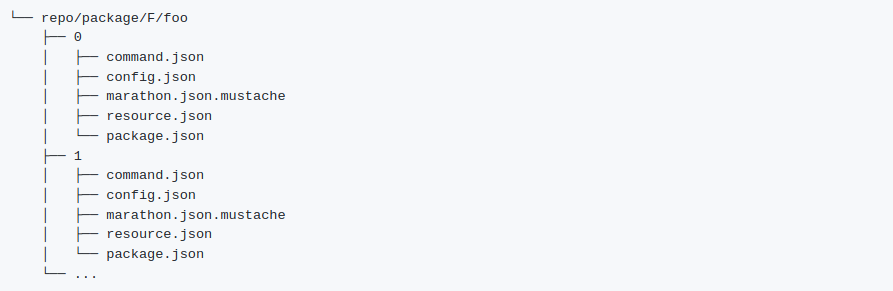
\includegraphics[scale=0.5,trim={0 0 20cm 0},clip ]{Pictures/Comparaison/deployer/universe/universe-repo.png}
\captionsetup{margin=1.5cm,format=hang,justification=justified}
\caption[]{Extrait des fichiers composant un Universe \newline}
\end{figure}

\paragraph{marathon.json.mustache:} Ce fichier est le template de l'application, qui une fois complété, créera une définition d'application Marathon capable de faire fonctionner le service. Les variables du marathon.json.mustache seront évaluées à partir d'un objet d'union créé en fusionnant trois objets dans l'ordre suivant :
\begin{itemize}
    \item Valeurs par défaut spécifiées dans le fichier config.json
    \item Les options fournies par l'utilisateur proviennent soit du DC/OS CLI (Command Ligne Interface ou interface en ligne de commande), soit du DC/OS UI (User Interface ou interface utilisateur)
    \item Le contenu de resource.json
\end{itemize}


\paragraph{config.json:} Ce fichier décrit les propriétés de configuration supportées par le package, représentées sous la forme d'un schéma json. Chaque propriété peut spécifier si elle est requise ou non, ainsi qu'une valeur par défaut.

Les utilisateurs peuvent ensuite remplacer des valeurs spécifiques au moment de l'installation en transmettant un fichier d'options à l'interface utilisateur du DC/OS ou en définissant des valeurs de configuration via l'interface utilisateur du DC/OS.

\paragraph{resource.json:} Ce fichier contient toutes les ressources hébergées en externe (par exemple les images Docker, les icônes, etc.) nécessaires à l'installation de l'application.

\paragraph{package.json:} Ce fichier contient des informations sur le package en question comme par exemple la version, son nom, etc.\newline 

\subsubsection{Installation}
Le catalogue Universe proposé par DC/OS contient environ 120 paquets que l'on peut exécuter uniquement depuis l'interface admin de DC/OS ou la CLI DC/OS.\footnote{On peut également remplir nous même le marathon.json.mustache et l'envoyer ensuite à l'API, mais on perd la notion de gestionnaire de paquets.}

\chapterimage{chapter-image/helm-01.jpg} 
\chapter{Compléments sur Helm}
\label{Helm}
\vspace{-2cm}
Helm est un projet opensource créé en 2015. C'est le gestionnaire de paquets recommandé par la CNCF (Cloud Native Computing Foundation) pour l'univers Kubernetes. C'est un projet implémenter en Go\footnote{Go est un langage de programmation compilé et concurrent inspiré de C et Pascal. Ce langage a été développé par Google.} (comme de nombreux projets qui gravitent autour de Kubernetes).\\

Helm est un SDK (Software Development Kit, un ensemble d’outils d’aide à la programmation) qui se découpe en 2 parties: 
\begin{itemize}
    \item Le client Helm est une ligne de commande pour l'utilisateur. La ligne de commande permet d'installer ou désinstaller des applications, d'installer automatiquement des dépendances applicatives, de mettre à jour des applications, de configurer des déploiements d'application, de récupérer des paquets d'application dans des dépôts, et enfin de communiquer avec la librairie Helm.
    \item La librairie Helm fournit la logique pour exécuter les commandes Helm. C'est la partie de Helm qui s'interface avec l'api-server de Kubernetes et qui permet de combiner les templates et la configuration des Charts pour créer des releases. C'est également elle qui implémente la logique de montée de version (rolling-update) ou de désinstallation des releases.
\end{itemize}

Helm s'accompagne de 3 concepts : les Charts, la config et la release. Nous allons parcourir ces différentes notions.

\subsubsection{Charts}
Les paquets Helm sont appelés des Charts et sont composés de plusieurs fichiers de configurations yaml (qui sont principalement des templates) et qui seront convertis en fichiers yaml compréhensible par Kubernetes grâce à la librairie Helm. La structure d'un Chart est la suivante :

\begin{itemize}
        \item charts/ : Les dépendances gérées manuellement peuvent être placées dans ce répertoire, bien qu'il soit généralement préférable d'utiliser dependencies dans Chart.yaml pour lier dynamiquement les dépendances.
        \item templates/ : Ce répertoire contient des fichiers templates qui vont être combinés avec des valeurs de configuration (provenant de values.yaml et de la ligne de commande) et rendus dans des manifestes Kubernetes. Ils contiennent en général au moins l'équivalent des trois fichiers basiques de Kubernetes : ingress, service et deployment. Les modèles utilisent le format de template du langage de programmation Go.
        \item Chart.yaml : Un fichier yaml contenant des métadonnées sur le Chart, telles que le nom et la version du Chart, des informations sur le créateur, un site web pertinent et des mots-clés de recherche, les dépendances du Chart.
      \item LICENCE : Une licence en texte clair pour le Chart.
     \item README.md : Un fichier readme avec des informations pour les utilisateurs du Chart.
      \item values.yaml : Un fichier YAML contenant les valeurs de configuration par défaut du Chart.\newline
\end{itemize} 

\begin{figure}[H]\centering
\renewcommand{\figurename}{Capture d'écran}
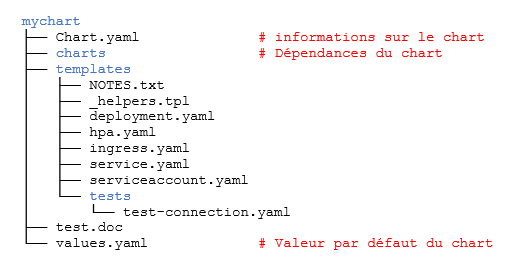
\includegraphics[scale=0.8]{Pictures/Comparaison/deployer/Kubernetes/helmChart.png}
\captionsetup{margin=1.5cm,format=hang,justification=justified}
\caption[]{Aperçu de l'ensemble des fichiers composant un Chart\newline
Remarque : Ici on a que les fichiers par défaut, dans la réalité il peut y en avoir beaucoup plus. \newline}
\end{figure}



L'ensemble des Charts est ensuite placé dans un Helm repository. Un Helm repository est un site HTTP qui délivre un fichier index.yaml et des Charts packagées. Ces fichiers peuvent être servis par n'importe quel serveur web, service de stockage d'objets ou un hôte de site statique tel que les pages GitHub(par exemple \url{https://inseefrlab.github.io/helm-charts-datascience/index.yaml}.

\subsubsection{Config et Release}
Helm permet de surcharger la configuration par défaut fourni avec un Chart. Cette surcharge peut s'effectuer de deux manières distinctes :
\begin{itemize}
    \item Par le biais d'un fichier values.yaml: l'utilisateur crée un fichier contenant les valeurs qu'il souhaite surcharger par rapport à la configuration par défaut.
    Il lui suffit alors de le préciser lors de l'installation du Chart \textit{Helm install chart mychart -f my-values.yaml}
    \item L'utilisateur peut également surcharger les valeurs de déploiement directement depuis la ligne de commande. On aurait donc (pour le même exemple que ci dessus) \textit{Helm install chart mychart --set ingress.enabled=true}.
    \item Enfin on peut également combiner les deux. \textit{Helm install chart mychart -f my-values.yaml --set ingress.enabled=true}.
\end{itemize}

Lorsque un Chart est installé dans le cluster, on parle alors de release. Une release est une instance d'un Chart exécuté dans un cluster Kubernetes. Un Chart peut souvent être installé plusieurs fois dans le même cluster. Et chaque fois qu'il est installé, une nouvelle release est créée.


\chapterimage{chapter-image/cloud.jpg} 
\chapter{GKE et Terraform : K8S en quelque clics}
\label{Terraform}
\vspace{-2cm}
\section*{Motivation}
Afin de pouvoir travailler sur Kubernetes à la fois depuis et hors de l'Insee, j'ai dans un premier temps utilisé minikube. Cette solution fonctionnait bien mais a vite présenté ses limites : environnement avec un seul node qui n'est pas du tout représentatif d'un environnement standard Kubernetes, et toute les configurations réalisée sur l'un des minikubes devait alors être réalisé sur l'autre.\newline

J'ai donc cherché une solution répondant aux critères suivant: je voulais avoir accès au cluster Kubernetes de n'importe où avec une configurations la moins dépendante possible du poste utilisé; les postes Insee fonctionnant sous Windows 7 avec des droits de base assez limité et un proxy, l'installation de tout les outils utilisés au cours de ce stage n'était pas facilitée. J'ai donc crée dans le cloud google une instance de vm ubuntu qui me servirait de point d'entrée pour mon futur cluster Kubernetes et sur laquelle j'installerai tout les outils nécessaires. Il me suffirait juste de me connecter a cet machine par ssh depuis n'importe quel ordinateur afin de bénéficier de tout ses outils.\newline


\section*{Gcloud}
Afin de répondre à ce besoin je me suis orienté vers Gcloud. Google Cloud est la plateforme qui regroupe les différents services cloud de Google. Gcloud propose différents services Cloud de calcul, de stockage, de networking, de Big Data, de machine Learning, d’internet des objets, de sécurité, de gestion cloud et de développement d’applications qui sont directement lancés sur les serveurs de Google. Cela permet donc à l'utilisateur de ne pas se soucier de la configuration des machines physique et de se concentrer uniquement sur le code de ce qu'il veut faire.\newline

On peut interagir avec Gcloud depuis l'interface prévu a cet effet ici \url{https://console.cloud.google.com/} ou bien par l'intermédiaire d'une CLI.\newline

Parmi les services proposés, 3 ont été utilisés : Compute engine afin de créer une instance de VM ubuntu me servant de point d'entrée dans le cluster, Google Kubernetes Engine pour créer un cluster Kubernetes et Cloud Dns pour assurer le routage de l'ensemble des requêtes vers le cluster et le service correspondant (cela nécessite au préalable de bénéficier d'un nom de domaine et de certificats\footnote{En effet le proxy utilisé par l'Insee n'accepte pas les sites web dont le certificat n'a pas été signé par une AC (authorité de confiance) reconnue. Pour obtenir un certificat, j'ai utilisé Let's Encrypt.} valides).\newline

Google Kubernetes Engine (GKE) permet de créer des clusters Kubernetes en quelques clics: l'utilisateur choisit un nom pour son cluster, la région dans laquelle le cluster sera déployé , et le nombre et la puissance des worker-nodes. En quelques minutes le cluster est alors configuré par Google et prêt à recevoir les premières requêtes.\newline

Comme tout les services Gcloud, GKE est un service pay-as-you-go (facturation à l’utilisation), afin de débourser le minimun j'éteignais donc régulièrement le cluster afin de "consommer" le moins possible. Le fait d'éteindre le cluster entraînait une perte de la configuration du cluster et je devais recommencer à chaque fois. J'ai donc cherché un outils me permettant d'automatiser cette phase.

\section*{Terraform}
Terraform est un outil d'infrastructure-as-code, open-source, et développé par Hashicorp qui permet d'automatiser la gestion d'une insfrastructure cloud, de plateformes, et de services. Il permet d'automatiser la configuration de VMs, ou de la création d'environnement cloud. \newline

Généralement, pour passer d'un état A à un état B, les outils semblables (tel que Chef ou Ansible) utilise un style de procédure où est décrit un code qui spécifie, étape par étape, comment atteindre un certain état final souhaité. Terraform (comme Puppet)  fonctionne différement, il repose sur un style plus déclaratif dans lequel un fichier contient le code qui spécifie l'état final souhaité. \newline

Pour cela Terraform fonctionne en 3 phases. Dans la première phase (dite de code), le développeur décrit l'état souhaité de son cluster ou de sa VM au sein de un ou plusieurs fichiers. Dans un second temps (phase plan), Terraform va comparer l'état actuel du cluster avec celui décrit au sein des fichiers de la première phase. Enfin dans un dernier temps (phase apply), il va appliquer les changements au cluster afin de le faire tendre vers l'état désiré. Au cours de cette partie Terraform peut nous renvoyer des variables qu'il aura générée (le lien du Kubernetes dashboard par exemple).\newline

Ces 3 phases sont facilités par la présence de modules (aussi appelés providers) fournit par la communauté et les fournisseurs cloud, afin de facilité l'interaction entre Terraform et la ressource que l'on veut modifier. On trouve donc un provider gcloud, AWS, (pour la configuration des clusters) mais aussi des providers Kubernetes (pour interagir avec l'API-server) ou un provider Helm afin de communiquer directement avec Helm.\newline

Grâce à Terraform nous avons pu écrire des scripts qui permettent de se créer un cluster Kubernetes pré-configuré et répondant a nos besoin en moins de 6 minutes, rejouable à l'infini et qui réponds à la logique devops. C'est à dire que l'ajout ou la modification d'une ressource ne relance pas toutes les phases et que l'ensemble du code peut donc être stocké dans un répertoire Git. Le répértoire contenant les codes Terraform du cluster GKE insee est disponible ici : \url{https://github.com/InseeFrLab/helm-charts}

\begin{figure}[H]\centering
\renewcommand{\figurename}{Schéma}
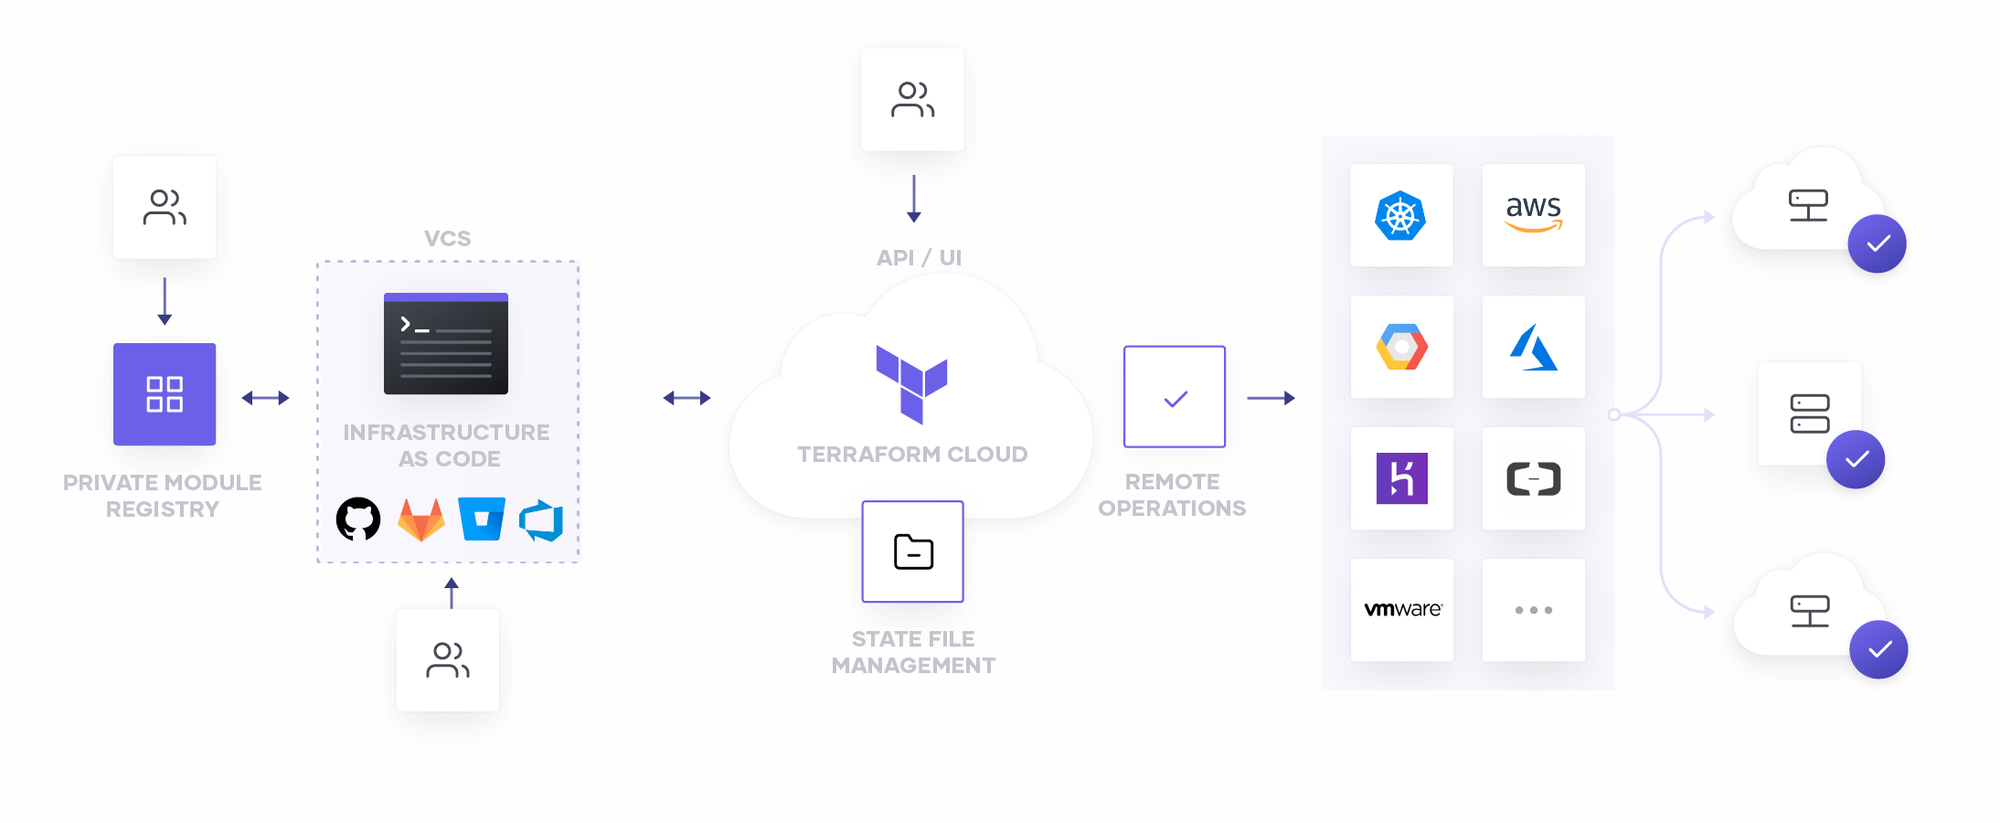
\includegraphics[angle=90, scale=0.35]{Pictures/annexe/terraform-cloud.png}
\captionsetup{margin=1.5cm,format=hang,justification=justified}
\caption[]{Schéma récapitulatif du fonctionnement de Terraform \newline}
\end{figure}




\chapterimage{/chapter-image/Kubeapps.png}
\chapter{Kubeapps une alternative à Onyxia ?}
\label{kubeapps}
\vspace{-2cm}
Dans le monde de Kubernetes, il existe des applications permettant de simplifier le déploiement de Charts Helm. On citera notamment Kubeapps ou encore Rancher. Kubeapps est une application déployable depuis Chart Helm qui permet de déployer une interface web permettant à son tour de déployer et de gérer des applications dans Kubernetes. Il permet d'ajouter des répertoires de Chart Helm (aussi bien public que privé) et de les déployer dans le cluster. Kubeapps permet également de gèrer, monter les versions, et supprimer les applications actuellement déployées dans le cluster. Cette application supporte également l'authentification OIDC ce qui nous permet d'utiliser Keycloak comme fournisseur d'identité.

\begin{figure}[H]\centering
\renewcommand{\figurename}{Capture d'écran}
\hspace{-1cm}
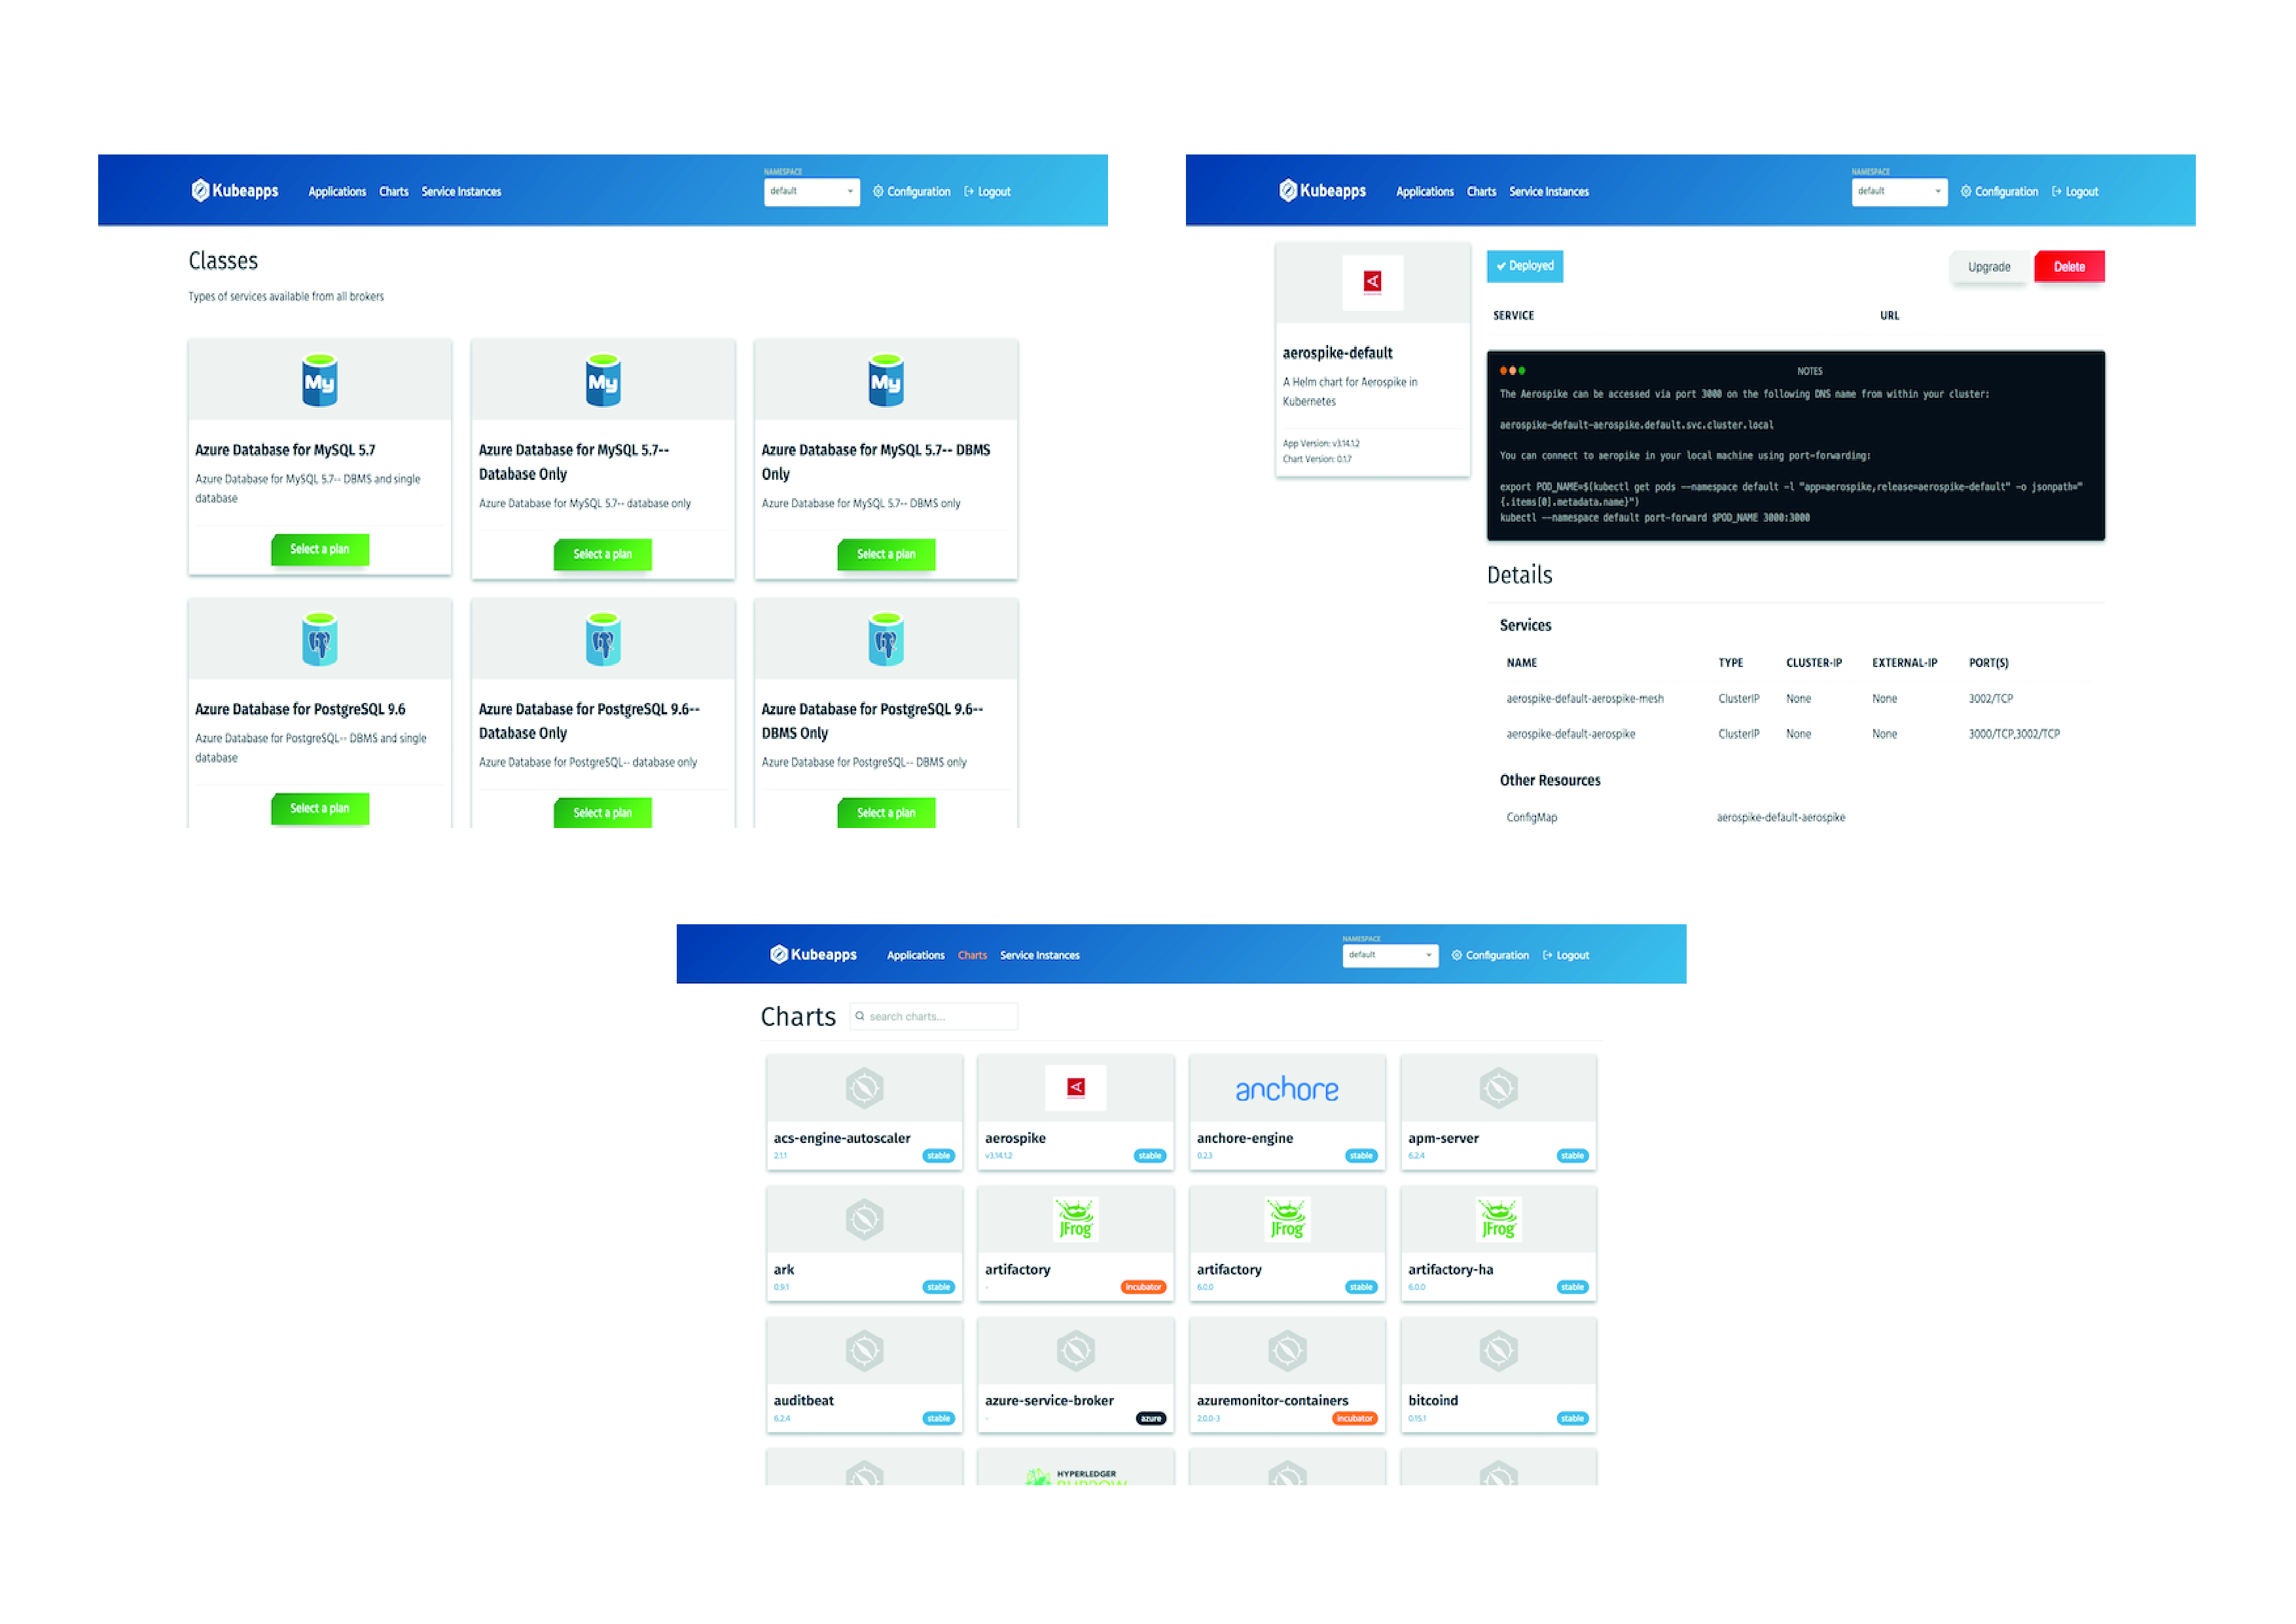
\includegraphics[scale=0.10]{Pictures/onyxia/kubeapps.jpg}
\captionsetup{margin=1.5cm,format=hang,justification=justified}
\caption[]{Aperçus de l'interface de Kubeapps \newline}
\end{figure}

\paragraph{Architecture}
Kubeapps est une application respectant l'architecture microservice. Elle est composée d'une ihm écrite en react/javascript (Kubeapps dashboard). Mais également d'une API écrite en Go (Kubeops), elle est en charge de la communication avec Helm 3 ou encore avec les différentes ressources Kubernetes (comme les AppRepositories ou les secrets).\\

\paragraph{Kubeapps un complément à Onyxia ?}
Kubeapps regroupe plusieurs fonctionnalité d'Onyxia : lister des services et les installer dans le cluster, consulter leur configuration et y accéder. Cependant ce dernier ne permet ni l'autoconfiguration ni de forcer certaines valeurs à la place de l'utilisateur (par exemple l'url du service). En effet, c'est à l'utilisateur de saisir la configuration (pour un postgres il faudrait notamment que l'utilisateur choisissent son mdp, son url, la taille de la bdd associées etc...). Utiliser Kubeapps comme une alternative à Onyxia n'est donc pas possible sans modifier son code source. Cela impliquerait de modifier le code de kubeops (l'API) écrit en Go, mais le rapport coût d'entrée et développement est relativement élevé, d'autant plus que le Go n'est pas courant à l'Insee (ce serait pour l'Insee une application difficilement maintenable).\newline

Une deuxième solution évoquée a été de faire interagir Onyxia directement avec l'API de Kubeapps. En effet on pourrait déployer Kubeapps dans le cluster et faire dialoguer Onyxia avec Kubeapps. Cela permettrait, d'une part au développeur de se connecter à Kubeapps à l'aide d'un token Kubernetes et de pouvoir configurer son application tel qu'il le souhaite, d'autre part au statisticien d'utiliser Onyxia pour déployer des services configurés rapidement. Onyxia devra néanmoins être capable de forcer certains paramètre pour chaque déploiement. L'API de Kubeapps nous servirait donc a installer le Chart, à lister ceux déja déployer, et à les supprimer. \\

Cette solution n'a finalement pas été retenue, en effet faire reposer Onyxia sur Kubeapps n'est pas forcement quelque chose de souhaitable puisque les différents endpoints de Kubeapps peuvent être amenés à évoluer. Kubeapps devenant juste un intermédiaire entre Helm et Onyxia, le coût pour qu'Onyxia  puisse dialoguer directement avec Helm ne nous paraissait pas important au point de retenir cette solution.\newpage

\begin{figure}[H]\centering
\renewcommand{\figurename}{Schéma}
\includegraphics[angle=90, scale=1]{Pictures/onyxia/Kubeapps.png}
\captionsetup{margin=1.5cm,format=hang,justification=justified}
\caption[]{Projet d'interfacage entre Onyxia et Kubeapps \newline}
\end{figure}





\chapterimage{chapter-image/security-01.jpg} 
\chapter{Orchestrateur et sécurité} 
\label{securite}
\vspace{-2cm}
De manière générale, la sécurité  a  pour  objectif  de réduire  les  risques pesant  sur  le  système    d’information,    pour limiter    leurs    impacts sur    le  fonctionnement et les activités métiers des organisations... Afin de disposer d’une infrastructure sécurisée des mesures doivent être mise en place afin de respecter les critères DICT. Pour rappel, voici la définition de ces critères :
\begin{itemize}
    \item \textbf{D}isponibilité : l’information doit être continuellement disponible.
    \item \textbf{I}ntégrité : l’information ne doit pas être altérée.
    \item \textbf{C}onfidentialité : l’information doit être uniquement accessible aux personnes autorisées.
    \item \textbf{T}raçabilité : Tous les mouvements de données doivent être tracés.\newline
\end{itemize}

Un orchestrateur de conteneurs permet d'optimiser des ressources en permettant l'exécution et l'ordonnancement des conteneurs sur un ensemble de machine. Sur chacune de ces machines, on trouve plusieurs couches: un OS (windows, linux, etc...) ainsi qu'un container runtime qui sera responsable de l'orchestration de nos conteneurs.\newline

Si l'on étudie plus en détail la constitution d'un conteneur, on s'aperçoit que ce dernier est lui aussi composé de plusieurs couches: une base de système d'exploitation, une runtime layer (jvm, node JS, etc...), et enfin la couche de l'application.  On retrouve d'ailleurs ces différentes couches lorsque l'on écrit un Dockerfile (le fichier permettant de créer l'image d'un conteneur).
\usemintedstyle{friendly}
\begin{minted}[mathescape,
               linenos,
               numbersep=5pt,
               gobble=2,
               framesep=2mm]{Bash}
    # Utilisation d'une image de base qui fournit l'environnement
    # runtime et les dépendances
    FROM adoptopenjdk:jre
    
    # On ajoute l'image de notre application
    COPY toto.jar /toto.jar
    
    # On modifie la configuration de l'environnement runtime 
    # ici on modifie le port d'écoute
    EXPOSE 8080
    
    # On lance l'appli
    ENTRYPOINT ["java","-jar","/toto.jar"]
\end{minted}

Chacune des couches présentées peuvent potentiellement introduire une faille de sécurité. Par exemple au niveau de l'infrastructure tout les composants peuvent présenter des failles, au niveau du Host OS, chaque distribution à ses failles de sécurité, et le container runtime n'est également pas épargné. Notre conteneur peut lui aussi présenter des failles. Au niveau de l'image de base qu'il utilise, en effet ces images dépendent généralement de d'autres images qui elles même vont dépendre de librairies de bases qui peuvent présenter des failles, il en va de même pour le runtime layer. Enfin la dernière couche, l'application layer regroupe les failles applicatives, "créée" par le développeur. 

\begin{figure}[H]\centering
\renewcommand{\figurename}{Tableau}
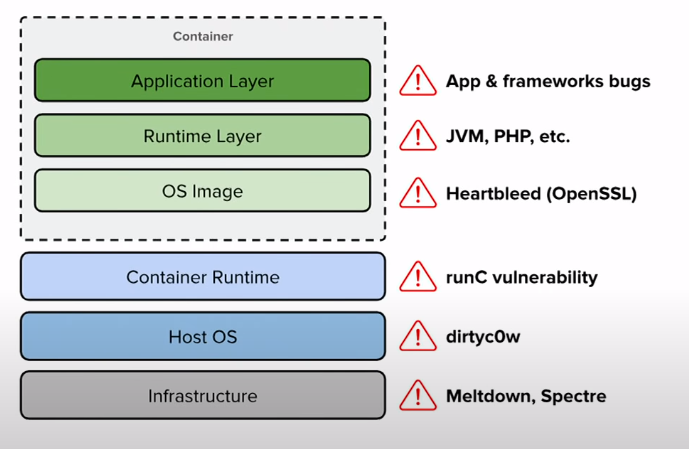
\includegraphics[scale=0.7]{Pictures/annexe/container-threat.PNG}
\captionsetup{margin=1.5cm,format=hang,justification=justified}
\caption[]{Exemple de menace sur chacune des couches intervenant dans un orchestrateur de conteneur. \newline
Source: La sécurité avec Kubernetes et les conteneurs Docker : une histoire sans fin (A. Roman C. Dubois)}
\end{figure}

Un environnement 100\% sécurisé n'existe pas, il existe pourtant des solutions assez simple pour réduire au maximun les risques. 

\section*{Quelques bonnes pratiques pour répondre au critère DICT}
\subsection*{Prometheus et Grafana}
Prometheus et Grafana sont des outils qui vont servir de surveillance de l'état du cluster, ils répondent à la problématique de disponibilité et de traçabilité.

Prometheus récupère toutes les métriques présentent dans le cluster dans lequel il s'exécute,  en passant par un composant qui s’appelle "Exporter". \newline

Ensuite il suffit d'interfacer Grafana avec Prometheus. Grafana peut s'interfacer avec plusieurs datasource (Google Cloud Monitoring, Azure monitor,...) dont Prometheus. Il faut ensuite mettre en forme les données récupérées sous forme de dashboard. On peut soit créer les dashboard soit même, soit en récupérer des déja fait par la communauté ici: \url{https://grafana.com/grafana/dashboards}.\newline 

Prometheus et Grafana s'installent facilement dans Marathon et ou Kubernetes. En effet, pour Marathon les deux sont disponible dans les paquets universes officiel, et pour Kubernetes plusieurs Charts Helm facilitent leur installation.

\begin{figure}[H]\centering
\renewcommand{\figurename}{Schéma}
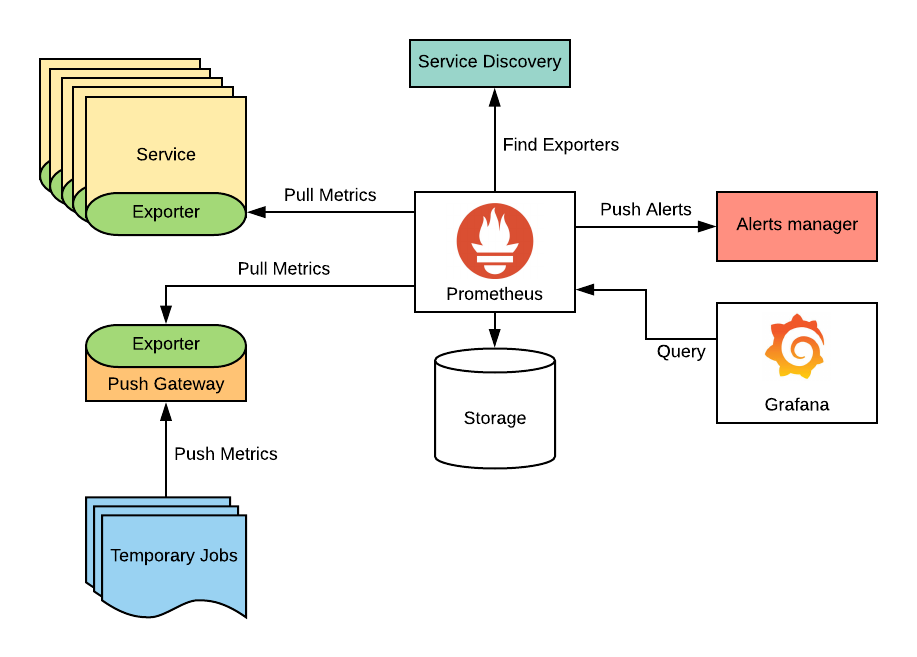
\includegraphics[scale=1]{Pictures/annexe/architecture.png}
\captionsetup{margin=1.5cm,format=hang,justification=justified}
\caption[]{Architecture générale de Prometheus et Grafana \newline}
\end{figure}

L'ensemble Prometheus et Grafana permet notamment de se prémunir de certains risques comme le manque de ressources, mais il ne protège pas de la perte soudaine d'une machine par exemple.\newline


\subsection*{Le chaos Engineering}
Plus récemment, une nouvelle discipline est apparue, initié par Netflix, le Chaos Engineering. Il a depuis été repris par plusieurs entreprises notamment Google, AWS, ou encore la SNCF. Le Chaos Engineering est défini de la manière suivante : \newline

\textit{ Le Chaos Engineering est la discipline de l'expérimentation sur un système
afin de renforcer la confiance dans les capacités du système
pour résister aux conditions turbulentes de la production. }\newline

L’expérience consiste donc à régulièrement choisir au hasard des instances dans l’environnement de production et de les mettre délibérément hors service et de voir comment l'environnement se comporte, et comment les équipes réagissent. Le but final étant de pouvoir, d'une part, mettre en place un système avec assez de redondance afin que l'utilisateur ne remarque rien, d'autre part, de créer des modèles de machines learning qui pourrait potentiellement repéré ce type de panne dans le futur. Il faut bien noter que de telle pratique ne sont pas (encore) mis en place sur la plateforme de l'innovation proposée par l'Insee.


\subsection*{Réaliser des sauvegardes des données}
La plateforme de l'innovation est une plateforme de tests, l'intégrité des données n'y est pour le moment pas garantie. En effet les services à la demande n'ont aucune vocation a être lancer éternellement.\newline

Afin de respecter le critère de l'intégrité il est important que tout ce qui s'exécute dans le cluster bénéficie de sauvegarde externe (pour les données des applications) et de redondance (à la fois pour les applications que pour les machines). Kubernetes permet par exemple de pouvoir créer des espaces de stockages qui peuvent être attaché au pods (donc volatile), dans des services de stockages externes (minIO), ou bien des espaces de stockages au sein de provider cloud (azure, aws, etc...). Marathon lui ne créé que des volumes de stockages propre a un node, une sauvegarde manuelle des espaces de stockages doit être faite afin de préserver les données en cas de pannes. 

\subsection*{Mise en place de gestion de droits et d'authentification}
Kubernetes comme Marathon permette chacun une authentification afin de pouvoir accéder au ressource et d'en limiter les accès. Marathon comme REST peuvent reposer sur de l'authentification OIDC (authentification à jeton). \newline

Cette authentification permet de mettre en place des mécanismes de réduction de droits, un utilisateur ne pouvant consulter les déploiements que d'un seul dossier ou namespace.\newline

La mise en place de tel mécanisme d'authentification permet par exemple a chaque utilisateur (ou application) de posséder ses propres secret (par exemple des properties ou des mots de passe) au sein de son namespace et uniquement accessible depuis ce namespace.


\subsection*{Se tenir à jour}
Chacun des composants du cluster doit toujours être maintenu dans sa version la plus récente. Par exemple Kubernetes sort une mise à jour de sa plateforme au moins une fois par mois. Ces mises à jour au delà des ajouts fonctionnels, apporte de nombreuses corrections de sécurité. Il en va de même pour les images utilisées pour créer nos conteneurs.

\subsection*{Vérifier ses sources}
Afin d'éviter la présence de faille au niveau de l'OS image (image qui sert de base à la création du conteneur), on peut par exemple mettre en place un registry Docker dit de confiance (On peut pour cela utiliser Harbor\footnote{un registre d'image docker, open source, qui sécurise les images grâce à des politiques et un contrôle d'accès basé sur les rôles, et qui garantit que les images soit exemptes de vulnérabilités, et qui signe les images comme étant de confiance}). C'est à dire qui contiendra uniquement des images qui auront été jugées sûres.\newline

Kubernetes (par rapport a Marathon) permet, par l'intermédiaire d'OPA (open policy agent), de mettre en place des règles de sécurité au sein du cluster. On pourra notamment mettre en place une règle qui limite l'utilisation des images venant de certains répertoires.



\chapterimage{chapter-image/autre-01.jpg} 
\chapter{Interfaçage avec le cloud }
\vspace{-2cm}
Dans cette parties nous aborderons divers points qui différencient Kubernetes et Marathon de DC/OS. Nous aborderons notamment la partie interfaçage avec le cloud.

\section*{Interfaçage avec le cloud}
Lorsqu'on choisit son orchestrateur de conteneur, on tient forcement compte de la facilité de déploiement de ce dernier. En effet, en général on veut que notre infrastructure soit déployable facilement, rapidement, et sans faire face à une très grande complexité de configuration.

\subsection*{Rappels : Paas, Saas, Iaas}
Avant de parler de comment déployer notre orchestrateur dans le cloud, revenons sur les différentes offres cloud qui existent. Le cloud permet d’entreposer sur des serveurs à distance des logiciels et des données. Les fournisseurs cloud proposent différentes types de services clouds. On retrouve:
\begin{itemize}
    \item Iaas (Infrastructure as a service) : Dans ce type d'offre, l'utilisateur doit configurer l'ensemble de l'infrastructure informatique. Cela concerne notamment les serveurs, le réseau, le stockage de données, ou encore la solution de virtualisation choisie. Cette offre cloud demande à l'administrateur de forte compétence tantôt sur les systèmes d'exploitations, les données ou encore sur le réseau. L'IAAS permet de dématérialiser l'ensemble de l'infrastructure matérielle.
    \item Paas (Plateform as a service): Dans cette solution, le fournisseur propose l'ensemble des solutions IAAS auxquelles il ajoute également la configuration des middleware : système d'exploitation, configuration réseau etc. Aucune configuration technique n'est requise.
    \item Saas (Software as a Service): Une solution SAAS regroupe l'ensemble des services SAAS et IAAS auxquelles s'ajoutent l'installation, la maintenance et la gestion des applications. Cette solution permet la simple utilisation des services et ne nécessite aucune expertise technique ou informatique. Par exemple, gmail est une application SAAS.\\
\end{itemize}


Dans le cas du développeur qui veut pouvoir déployer rapidement ces applications, il est intéressant d'avoir accès à une offre Paas.
\newpage
\begin{figure}[H]\centering
\renewcommand{\figurename}{Schéma}
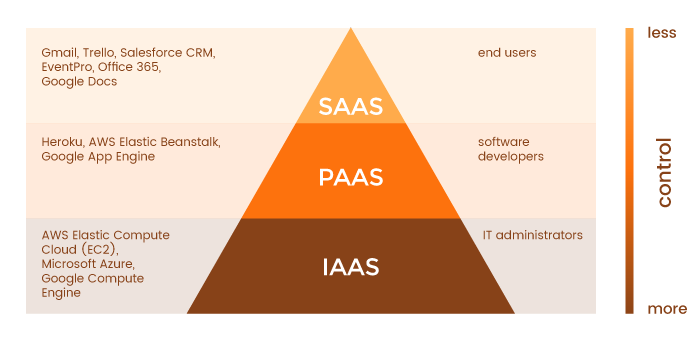
\includegraphics[clip,trim={0cm, 0cm, 0cm, 1cm}, scale=0.6]{Pictures/Comparaison/cloud/difference-cloud.png}
\captionsetup{margin=1.5cm,format=hang,justification=justified}
\caption[]{Différence entre offre Cloud Iaas, Saas et Paas \newline}
\end{figure}

\vspace{-1cm}
\subsection*{Offre Cloud Marathon et Kubernetes}
De part son succès, de nombreux provider cloud proposent une offre Kubernetes, parmi eux on peut citer : Microsoft Azure, Amazon EKS (Amazon Elastic Kubernetes Service), GKE (Google Kubernetes Engine), etc. Ces offres proposent de créer des clusters Kubernetes en quelques minutes seulement. Par exemple, il suffit de quelque clics (choix du nombre et du type des workers nodes, localisation du cluster et la version de Kubernetes) pour lancer un cluster Kubernetes dans GKE. Ici, on parle d'offre Paas (ou clés en main). En effet, une fois le cluster créé, le développeur peut directement y déployer ses applications.\\

Pour le développeur qui veut tester Kubernetes sans avoir à lancer un cluster dans le cloud, de nombreuse solutions existent pour lancer un cluster Kubernetes en local : minikube avec virtualbox, k3s avec docker. Ces offres proposent des clusters Kubernetes déjà configurés avec un seul worker node, permettant au développeur de tester facilement les possibilités que peut offrir Kubernetes.\\

Kubernetes centralise l'ensemble des providers cloud qui fournissent des solutions ici : \url{https://Kubernetes.io/fr/docs/setup/pick-right-solution/}. \\

A l'inverse, pour Marathon il n'existe pas de solution Paas. Le seul moyen de lancer un cluster Mesos avec Marathon dans le cloud est de souscrire à une offre Iaas. Par la suite, l'utilisateur doit configurer ses machines, en y installant l'ensemble des briques Mesos ou en utilisant l'outil d'installation DC/OS. De la même façon, il est impossible de lancer un cluster Mesos avec Marathon en local sans devoir configurer l'ensemble de la sphère Mesos\footnote{\url{http://www.lordofthejars.com/2015/04/apache-mesos-marathon-and-java-ee.html} pour une utilisation en local}. Cette différence s'explique notamment par le fait que les utilisateurs de Mesos, n'utilisent pas ce dernier uniquement pour avoir Marathon comme framework. Le provider cloud n'a donc aucun intêret à proposer une offre packagée.\\

Par ailleurs, il peut être intéressant d'automatiser la phase de création d'un cluster Kubernetes ou DC/OS (voir annexe \ref{Terraform}). Il existe 2 principaux outils qui répondent à de tels besoin: Terraform et Ansible. Généralement, on pourra utiliser Terraform et/ou Ansible avec k8s alors que DC/OS ne sera compatible qu'avec Ansible.


\chapterimage{/chapter-image/glossaire.png}
\printglossaries
\addcontentsline{toc}{chapter}{\textcolor{ocre}{Glossaire}}
%----------------------------------------------------------------------------------------
%	BIBLIOGRAPHY
%----------------------------------------------------------------------------------------

\chapterimage{/chapter-image/bibliography.png}
\chapter*{Bibliographie}
\addcontentsline{toc}{chapter}{\textcolor{ocre}{Bibliographie}}
\nocite{*}
\vspace{-2cm}
\printbibliography[heading=bibempty]

%----------------------------------------------------------------------------------------
%	INDEX
%----------------------------------------------------------------------------------------

\cleardoublepage
\phantomsection
\setlength{\columnsep}{0.75cm}
\addcontentsline{toc}{chapter}{\textcolor{ocre}{Index}}
\printindex

%----------------------------------------------------------------------------------------

\end{document}
